\documentclass[11pt,titlepage,a4paper]{book}
\usepackage[T1]{fontenc}
\usepackage[utf8]{inputenc}
\DeclareUnicodeCharacter{202F}{ }
\usepackage[french]{babel}

\usepackage{calc}
\usepackage{graphicx}
\usepackage{amsmath}
\usepackage{amssymb}
\usepackage{overpic}
\usepackage{color}
\usepackage{rotate}
\usepackage[most]{tcolorbox}
\usepackage{multirow}
\usepackage{mychapter,mymacros}
\usepackage{makeidx}
\usepackage{pdfpages}
\usepackage{lscape}

\input{PhS_Header}

\usepackage{longtable}
\usepackage{array}
\usepackage{booktabs}
\usepackage{xcolor}
\usepackage{colortbl}
\usepackage{float}
\usepackage{placeins}
\usepackage{tabularx}

\usepackage{latexsym}
\usepackage{algorithm}
\usepackage{minitoc}
\dominitoc
\setcounter{minitocdepth}{2}
\setcounter{secnumdepth}{3}

\usepackage[babel=true]{csquotes}
\usepackage{setspace}
\setlength{\parskip}{0pt}
\setlength{\parindent}{15pt}
\onehalfspacing
\usepackage{algorithmicx}
\usepackage{algpseudocode}
\usepackage{hyperref}
\usepackage{fancybox}
\usepackage{enumitem}
\usepackage{verbatim}

\setstretch{1.15}
\graphicspath{{figures/}}

\definecolor{grisclair}{gray}{0.2}
\definecolor{light-gary}{gray}{0.95}
\definecolor{lgray}{gray}{0.85}
\definecolor{gris}{gray}{0.45}

\usepackage[backend=biber,style=numeric]{biblatex}
\addbibresource{Thesis-report.bib}
\addbibresource{webographie.bib}

\oddsidemargin 10.0mm
\evensidemargin 10.0mm
\textheight 220.0mm
\textwidth 145.0mm

\newenvironment{remarque}{\textbf{Remark:}}{}

\newlength{\longueurequation}
\newlength{\longueurrestante}

\newcommand{\me}[1]{%
\longueurrestante=\linegoal%
\settowidth{\longueurequation}{$#1$}%
\ifthenelse{\longueurequation>\longueurrestante}{\begin{displaymath} #1 \end{displaymath}}{$#1$}%
}

\setlength\belowcaptionskip{0.25cm}
\everymath{\displaystyle}

\begin{document}

\includepdf{Chapitres/Page_garde_BC.pdf}

\thispagestyle{empty}
\chapter*{Déclaration sur l’utilisation de l’intelligence artificielle générative}

Nous déclarons par la présente avoir utilisé des outils d’intelligence artificielle générative (IAG) comme suit :

\begin{enumerate}
	\item \textbf{Reformulation :} nous avons fait appel à \textbf{ChatGPT (OpenAI)} pour corriger et améliorer certaines parties rédactionnelles du rapport, tout en garantissant la clarté et la cohérence du contenu.
	
	\item \textbf{Assistance au développement :} nous avons utilisé \textbf{ChatGPT (OpenAI)} comme assistant afin de comprendre certaines parties techniques, corriger des erreurs et organiser certaines fonctionnalités du projet.
	
	\item \textbf{Organisation et documentation :} les outils d’IA ont également été utilisés pour aider à structurer certaines sections du rapport et reformuler des descriptions techniques.
\end{enumerate}

Les contenus générés ont été vérifiés, adaptés et validés par les auteurs du projet avant leur intégration dans ce rapport.

\thispagestyle{empty}
\chapter*{\centering \Huge \textbf{DÉDICACE}}

\vspace{0.5cm}

\begin{center}
	{\LARGE\bfseries \textarabic{✧ أول أفراح العمر ✧}}
\end{center}

\vspace{0.8cm}

\begin{center}
	\large\itshape
	« Aucun mot ne pourra exprimer toute la gratitude et l’amour que je porte dans mon cœur. »
\end{center}

\vspace{1cm}

\begin{center}
	\textbf{\large À ma chère mère}
\end{center}

Aucun mot ne pourra exprimer tout l’amour et la gratitude que je ressens envers toi. Merci pour tous les sacrifices, ta patience et tous les efforts que tu as faits afin de me voir réussir. Ton amour et tes prières ont toujours été ma plus grande force. Tout ce que je suis aujourd’hui, je le dois à toi.
\vspace{0.7cm}

\begin{center}
	\textbf{\large À mon grand frère Imed}
\end{center}

merci d’avoir toujours été présent à mes côtés dans les moments difficiles comme dans les plus beaux. Merci pour ton soutien, ta patience et tous les efforts que tu as faits pour moi. Ta présence dans ma vie représente une grande source de force et de motivation.


\vspace{0.7cm}

\begin{center}
	\textbf{\large À mon petit frère Haroun}
\end{center}

merci pour tous les moments de joie et de bonheur que tu apportes dans ma vie. Ta présence me donne toujours le sourire.

\vspace{0.7cm}

\begin{center}
	\textbf{\large À mes meilleures amies Imen et Roya ♡}
\end{center}

merci pour votre soutien, votre amour sincère et tous les beaux souvenirs que nous avons partagés ensemble. Votre présence a beaucoup compté pour moi.

\vspace{0.7cm}

\begin{center}
	\textbf{\large À mes chères tantes Saida , Najwa et Monia ♡}
\end{center}

merci pour toute la tendresse, l’affection et le soutien que vous m’avez offerts. Votre présence et votre bienveillance occupent une place très spéciale dans mon cœur.

\vspace{0.7cm}

\begin{center}
	\textbf{\large À Becha $\heartsuit$}
\end{center}

merci pour ta présence, ton soutien, ton écoute et tous les moments qui m’ont donné la force d’avancer et de croire davantage en moi-même. Merci d’avoir été une source de motivation et de réconfort durant ce parcours.

\vspace{0.7cm}

\begin{center}
	\textbf{\large Et enfin, au Club Africain}
\end{center}

plus qu’un simple club, une passion qui vit en moi depuis toujours, une source de joie, de fierté et d’émotions indescriptibles. Le Club Africain restera toujours une partie de mon cœur et de mon identité.

\vfill

\begin{flushright}
	\textit{\large Avec tout mon amour et ma gratitude.}
	
	\vspace{0.4cm}
	
	\textbf{Ameni Nagati}
\end{flushright}²²²
\newpage
\thispagestyle{empty}

\begin{center}
	
	{\Huge \textbf{DÉDICACE}}
	
	\vspace{1cm}
	
	{\large\bfseries 🎓 \textarabic{أول أفراح العمر} 🎓}
	
	\vspace{0.8cm}
	
	\textit{« La réussite n’a de valeur que lorsqu’elle est partagée avec ceux qui nous ont soutenus et aimés tout au long du chemin. »}
	
\end{center}
\begin{center}
	\textbf{\Large À mes chers parents}
\end{center}

Que nulle dédicace ne puisse exprimer mes sincères sentiments, mon profond amour et mon immense gratitude envers vous.  
Merci pour votre patience, vos sacrifices, vos encouragements et votre soutien inconditionnel tout au long de mon parcours.  
Sans vous, je ne serais jamais arrivée là où je suis aujourd’hui.

\vspace{0.7cm}

\begin{center}
	\textbf{\Large À mes chers grands-parents}
\end{center}

Pour leur affection, leurs prières et leur présence précieuse dans ma vie.

\vspace{0.7cm}

\begin{center}
	\textbf{\Large À mon cher frère et ma chère sœur}
\end{center}

Merci pour votre amour, votre soutien et tous les moments de motivation et de réconfort que vous m’avez apportés.

\vspace{0.7cm}

\begin{center}
	\textbf{\Large À mes chers amis}
\end{center}

Qui, grâce à leurs encouragements et leur présence, ont contribué à rendre cette aventure plus belle et inoubliable.

\vspace{0.7cm}

\begin{center}
	\textbf{\Large À toute ma famille et à tous ceux que j’aime}
\end{center}

Merci pour votre confiance, votre affection et votre soutien tout au long de ce parcours.

\vfill

\begin{flushright}
	\textit{Avec tout mon amour et ma reconnaissance,}
	
	\vspace{0.3cm}
	
	\textbf{Emna Benharb}
\end{flushright}

\thispagestyle{empty}
\chapter*{Remerciements}

Nous remercions tout d’abord le bon Dieu pour l’achèvement de ce projet de fin d’études.

Nous tenons tout d’abord à exprimer nos remerciements les plus chaleureux à Mme \textbf{Chourouk Hammami}, notre encadrante à l’École Supérieure d’Économie Numérique (ESEN), pour sa confiance, son encadrement enrichissant, son soutien inconditionnel ainsi que pour l’attention et le temps qu’elle nous a accordés tout au long de la réalisation de ce projet. Nous la remercions également pour ses précieux conseils, ses orientations et ses corrections qui nous ont permis d’améliorer la qualité de notre travail.

Nous adressons également nos sincères remerciements à M. \textbf{Bassem Thabti}, notre encadrant au sein de la société \textbf{Virtual Dev}, qui n’a épargné aucun effort pour nous soutenir et nous orienter durant toute la période du PFE. Nous le remercions pour son aide précieuse, sa disponibilité, sa bienveillance ainsi que pour la confiance qu’il nous a accordée afin de réaliser ce projet dans les meilleures conditions.

Nous tenons également à remercier le président du jury d’avoir accepté la lourde tâche de juger notre travail et de présider notre soutenance.

Nous adressons aussi nos remerciements à l’examinateur pour avoir accepté d’évaluer et de juger notre rapport de projet de fin d’études.

Nous remercions également tout le personnel de la société \textbf{Virtual Dev}, qui nous a aidés de près ou de loin à l’élaboration de ce travail, ainsi que tous les collaborateurs qui ont contribué au bon déroulement de notre stage.

Nous devons aussi notre réussite à nos familles qui n’ont cessé de nous soutenir et de nous encourager durant tout notre parcours universitaire.

Enfin, nous adressons nos chaleureux remerciements à tous nos enseignants ainsi qu’aux responsables de l’administration de l’École Supérieure d’Économie Numérique (ESEN) pour la qualité de la formation qu’ils nous ont offerte.

\thispagestyle{empty}
\begin{center}
	\textbf{\Large Résumé}
\end{center}

\vspace{0.5cm}

\begin{tcolorbox}[colback=gray!5,colframe=black]
	
	Ce projet consiste à développer une plateforme intelligente permettant d’automatiser le traitement des factures fournisseurs à l’aide des technologies OCR et Intelligence Artificielle. La solution permet l’extraction automatique des données, la détection des anomalies ainsi que la validation financière des factures.
	
	L’application a été développée avec React pour le frontend, FastAPI pour le backend et PostgreSQL pour la gestion de la base de données.
	
	\vspace{0.3cm}
	
	\textbf{Mots clés :} OCR, Intelligence Artificielle, React, FastAPI, PostgreSQL, Factures fournisseurs.
	
\end{tcolorbox}

\vspace{1cm}

\begin{center}
	\textbf{\Large Abstract}
\end{center}

\vspace{0.5cm}

\begin{tcolorbox}[colback=gray!5,colframe=black]
	
	This project aims to develop an intelligent platform for automating supplier invoice processing using OCR and Artificial Intelligence technologies. The solution allows automatic data extraction, anomaly detection and financial validation of invoices.
	
	The application was developed using React for the frontend, FastAPI for the backend and PostgreSQL for database management.
	
	\vspace{0.3cm}
	
	\textbf{Keywords :} OCR, Artificial Intelligence, React, FastAPI, PostgreSQL, Supplier invoices.
	
\end{tcolorbox}

\pagestyle{headings}
\pagenumbering{roman}

\tableofcontents
%\listoftables
\thispagestyle{empty}
%\listoffigures
\thispagestyle{empty}

\include{Chapitres/Notations}

\pagenumbering{arabic}

\chapter*{Introduction Générale}

Aujourd'hui, les entreprises digitalisent leurs processus. Les entreprises digitalisent leurs processus pour gagner du temps, réduire les erreurs et améliorer l'efficacité.

Le processus Inovice IA gère les factures fournisseurs depuis leur réception jusqu’à leur validation. Le processus Inovice IA constitue une étape clé de la gestion financière. Dans de nombreuses entreprises, le processus Inovice IA reste encore manuel ou peu automatisé. Le processus Inovice IA provoque des retards, génère des erreurs et réduit la visibilité.

Dans ce contexte, le projet se déroule au sein de l’entreprise \textbf{Virtuel Dev}. Le projet consiste à créer une plateforme qui utilise l’intelligence artificielle pour automatiser le traitement des factures fournisseurs.

La solution traite plusieurs types de factures (PDF, images, XML). La solution utilise l’OCR pour extraire les informations et l’intelligence artificielle pour analyser les données, classer les charges et détecter les anomalies.

L’application utilise une architecture simple : un frontend en \textbf{React}, un backend en \textbf{FastAPI (framework Python)} et une base de données \textbf{PostgreSQL}.

Cette fonction permet :
\begin{itemize}
\item d’importer les factures des fournisseurs ;
\item extraire automatiquement les informations clés ;
\item Classer les charges de façon intelligente ;
\item détecter les anomalies (TVA, montants, doublons) ;
\item Aider à la prise de décision pour la validation.
Voici la réponse de l'utilisateur :

\end{itemize}

Le projet vise à offrir une solution simple, fiable et intelligente. La solution facilite le traitement des factures, améliore le travail des utilisateurs et garantit une meilleure traçabilité.

Nous avons structuré le rapport ainsi :

\begin{itemize}

\item Le premier chapitre présente le cadre général du projet et l’entreprise d’accueil.

\item Le deuxième chapitre présente l’analyse et la conception du système. Le deuxième chapitre expose les besoins fonctionnels et non fonctionnels, l’architecture du système et la planification des sprints.

\item Le troisième chapitre présente le Sprint 1 dédié à l’authentification, à la gestion des utilisateurs et à l’extraction des données.

\item Le quatrième chapitre présente le Sprint 2 qui se consacre au traitement et à la consultation des données extraites.

\item Le cinquième chapitre présente le Sprint 3 qui porte sur la validation financière et la traçabilité des actions.

\end{itemize}
\chapter{Cadre général du projet}

%====================================================
\section{Introduction}
%====================================================

Le premier chapitre présente le contexte général du projet. Nous commençons par une présentation de l’entreprise d’accueil, puis nous décrivons le projet, la problématique étudiée ainsi que la solution proposée. Enfin, nous présentons la méthodologie adoptée durant le développement.

%====================================================
\section{Présentation de l’entreprise}
%====================================================

Le projet a été réalisé au sein de l’entreprise \textbf{Virtual Dev}, une société spécialisée dans le développement des applications web et des solutions intelligentes. L’entreprise accompagne les organisations dans leur transformation digitale à travers des solutions innovantes basées sur les technologies modernes et l’intelligence artificielle.

\begin{figure}[H]
	\centering
	
\includegraphics[width=0.15\textwidth]{logo_virtualdev.png}
	\caption{Logo de l’entreprise Virtual Dev}
	\label{fig:logo_virtualdev}
\end{figure}

\FloatBarrier

%====================================================
\subsection{Domaines d’intervention}
%====================================================

Virtual Dev possède plusieurs domaines d’intervention dans le secteur des technologies numériques. L’entreprise travaille notamment dans le développement web, les plateformes SaaS, l’intelligence artificielle, l’automatisation des processus métiers, l’analyse des données ainsi que les systèmes de gestion, comme présenté dans la figure \ref{fig:domaines_intervention}.

\begin{figure}[H]
	\centering
	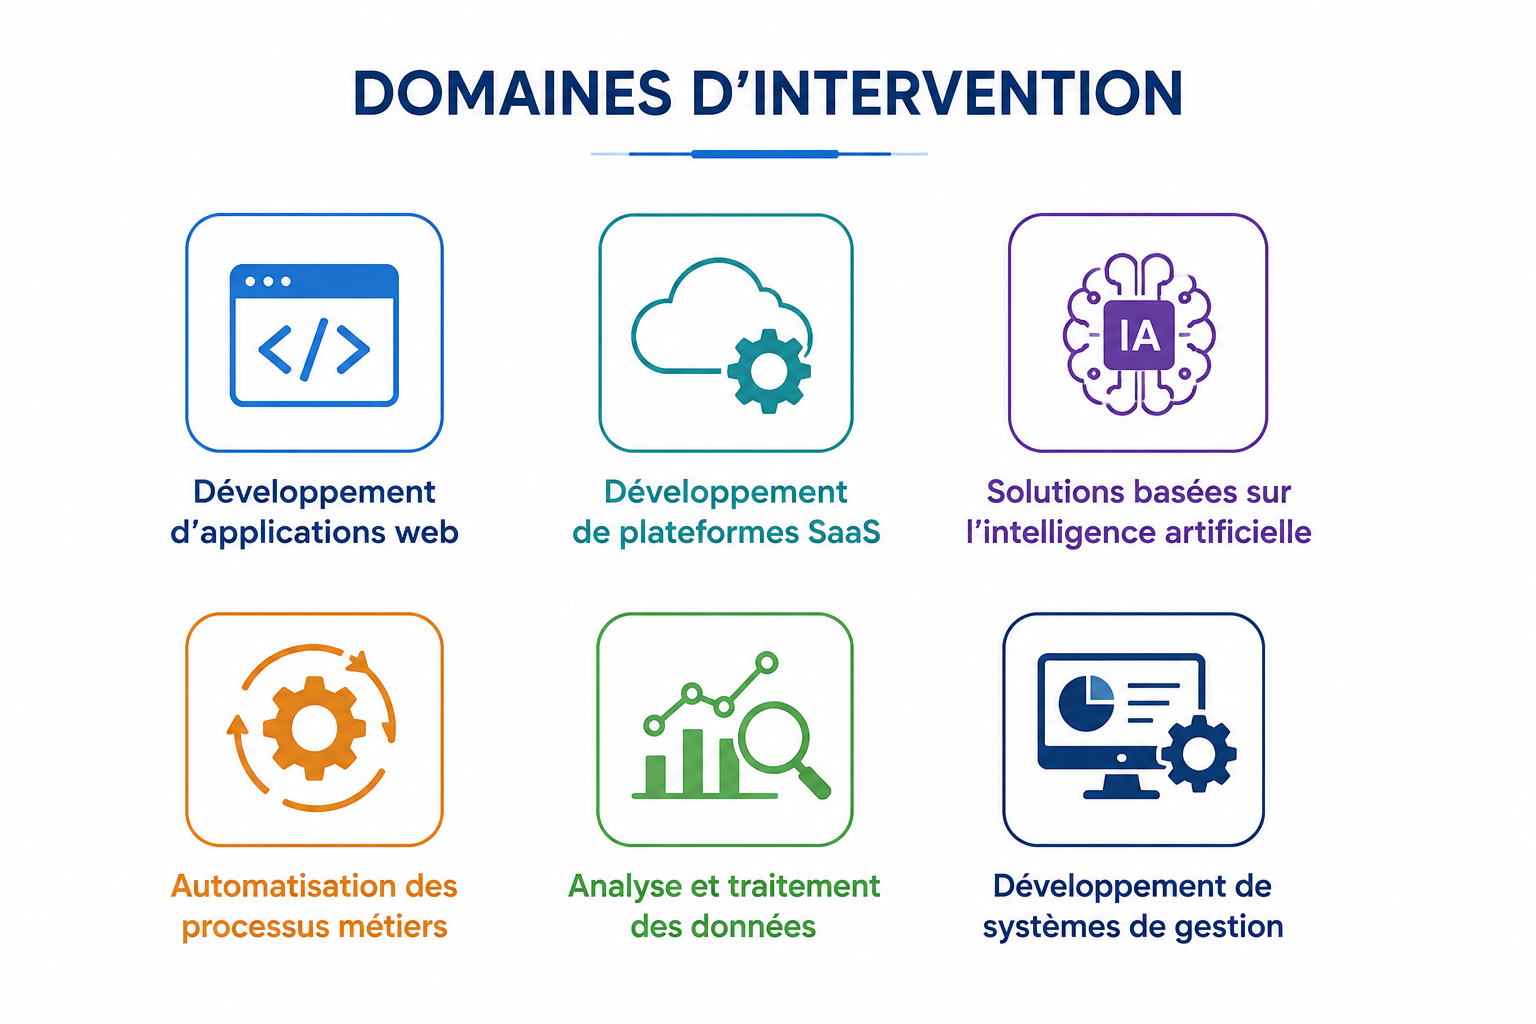
\includegraphics[width=0.6\textwidth]{domaines_intervention_simple.png}
	\caption{Principaux domaines d’intervention de l’entreprise}
	\label{fig:domaines_intervention}
\end{figure}

\FloatBarrier

%====================================================
\section{Objectif du projet}
%====================================================

L’objectif principal de ce projet est de concevoir et développer une plateforme intelligente permettant l’automatisation du processus de traitement des factures et des opérations financières au sein d’une entreprise.

Cette solution vise à réduire les tâches manuelles, améliorer la rapidité de traitement des documents et limiter les erreurs humaines grâce à l’intégration des technologies d’intelligence artificielle et de reconnaissance optique de caractères (OCR).

La plateforme développée permet également de centraliser les informations financières, gérer les utilisateurs selon leurs rôles, assurer le suivi des validations et des actions effectuées, ainsi que faciliter la consultation et l’analyse des données via des tableaux de bord interactifs. À travers ce projet, nous cherchons à offrir une solution moderne, sécurisée et performante capable d’optimiser la gestion financière et d’améliorer la productivité des utilisateurs.

%====================================================
\section{Étude de l’existant}

\subsection{Contexte}
%====================================================

Le traitement manuel des factures fournisseurs reste une tâche longue et répétitive. Les utilisateurs doivent vérifier les informations, saisir les données et suivre les validations financières. Ce mode de fonctionnement entraîne plusieurs problèmes tels que les retards de traitement, les erreurs humaines, la difficulté de détecter les anomalies ainsi qu’un manque de traçabilité des opérations. De plus, l’absence d’automatisation réduit l’efficacité du processus et augmente le risque d’erreurs dans la gestion financière, comme illustré dans la figure \ref{fig:processus_actuel}.

\begin{figure}[H]
	\centering
	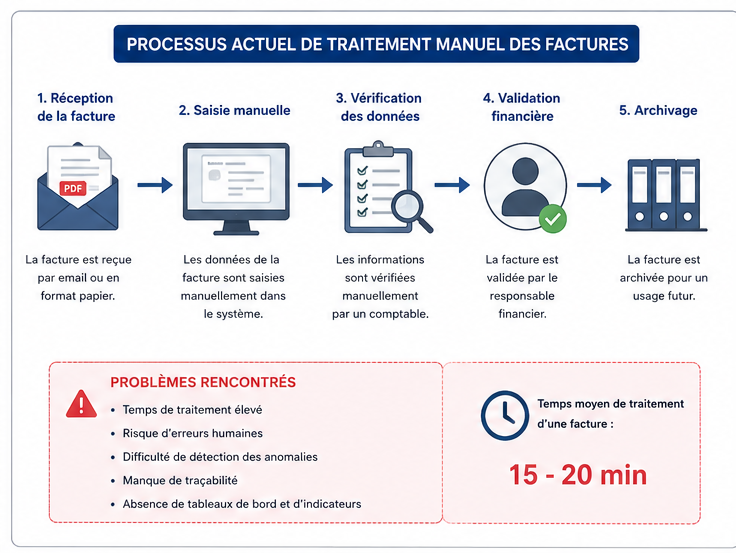
\includegraphics[width=0.7\textwidth]{processus_actuel.jpg}
	\caption{Processus actuel de traitement manuel des factures}
	\label{fig:processus_actuel}
\end{figure}

\FloatBarrier

%====================================================
\section{Problématique}
%====================================================

Dans un contexte de transformation numérique des entreprises, la gestion manuelle des factures et des documents financiers représente encore une contrainte importante pour plusieurs organisations.

Les processus traditionnels basés sur la saisie manuelle des données, la vérification humaine et le traitement papier engendrent des pertes de temps, des erreurs de saisie ainsi qu’un manque de traçabilité des opérations financières.

De plus, la multiplication des documents à traiter rend le suivi des validations et des décisions financières plus complexe, ce qui impacte la productivité et la fiabilité des services comptables et administratifs.

Par ailleurs, l’absence d’un système intelligent capable d’automatiser l’extraction et l’analyse des données des factures limite la rapidité de traitement et augmente les risques d’erreurs.

Les entreprises ont alors besoin d’une solution moderne permettant d’automatiser les différentes étapes du processus d’achat et de validation financière tout en assurant la sécurité, la centralisation des informations et la traçabilité des actions effectuées.

Afin de répondre à ces besoins, notre projet consiste à développer une plateforme intelligente basée sur l’intelligence artificielle et les technologies OCR permettant l’automatisation du traitement des factures, la gestion des utilisateurs, le suivi des validations financières ainsi que la visualisation des données à travers des tableaux de bord interactifs.

%====================================================
\section{Solution proposée}
%====================================================

Afin de répondre aux problématiques identifiées, nous proposons une plateforme intelligente dédiée à l’automatisation du traitement des factures fournisseurs.
Cette solution repose sur l’intégration des technologies OCR et de l’intelligence artificielle afin d’extraire, analyser et valider automatiquement les données financières. La plateforme permet également d’assurer la gestion des utilisateurs, le suivi des validations, la centralisation des informations ainsi que la visualisation des statistiques à travers des tableaux de bord interactifs. L’objectif principal de cette solution est d’améliorer la rapidité, la fiabilité et la traçabilité des opérations financières au sein de l’entreprise.

%====================================================
\subsection{Workflow global du système}
%====================================================

Le workflow global du système présenté ci-dessous illustre les différentes étapes du traitement automatisé des factures au sein de la plateforme. Il décrit le processus depuis l’importation des documents, l’extraction et l’analyse des données par OCR et intelligence artificielle, jusqu’à la validation financière, la visualisation des statistiques et l’archivage des informations traitées. Cette automatisation permet de réduire le temps de traitement, limiter les erreurs humaines, améliorer la traçabilité des opérations et faciliter la prise de décision financière. Elle offre également une meilleure organisation des données ainsi qu’un suivi plus efficace des factures, comme présenté dans la figure \ref{fig:workflow}.

\begin{figure}[H]
	\centering
	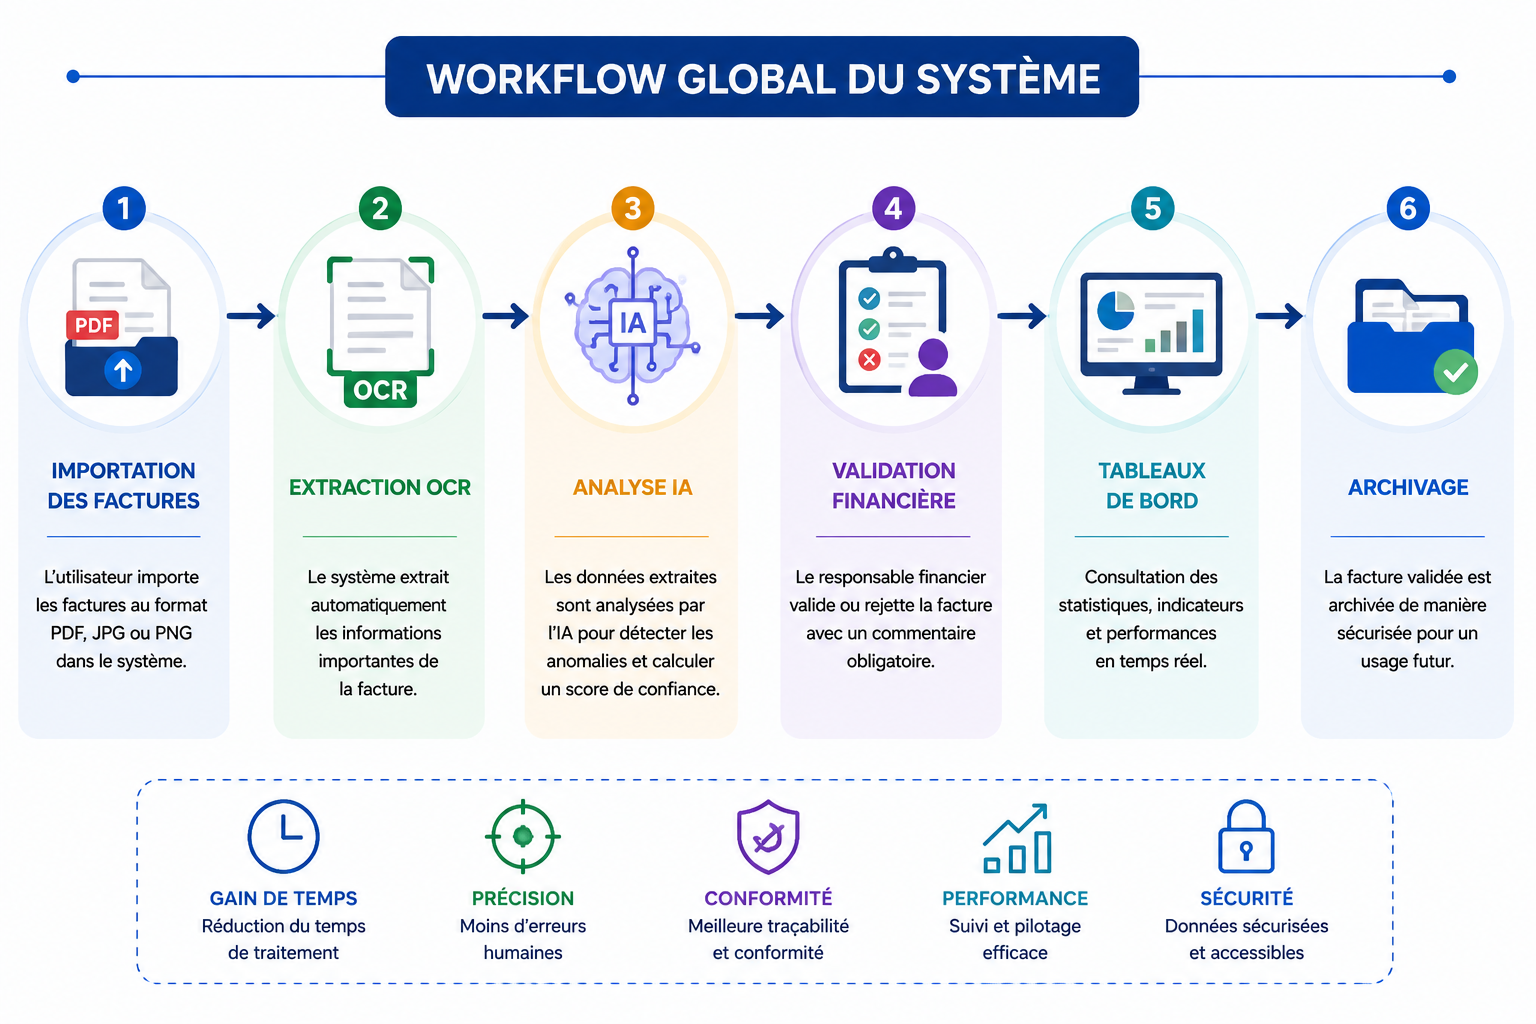
\includegraphics[width=0.7\textwidth]{workflow_systeme.jpg}
	\caption{Workflow global du système}
	\label{fig:workflow}
\end{figure}

\FloatBarrier

%====================================================
\subsection{Architecture générale}
%====================================================

L’architecture générale de la solution proposée repose sur une organisation modulaire permettant d’assurer la communication entre les différentes composantes du système. Elle intègre une interface frontend pour les utilisateurs, un backend assurant la logique métier, une base de données pour le stockage des informations ainsi que des services d’intelligence artificielle et d’OCR destinés au traitement automatisé des factures. comme illustré dans la figure \ref{fig:architecture_generale}

\begin{figure}[H]
	\centering
	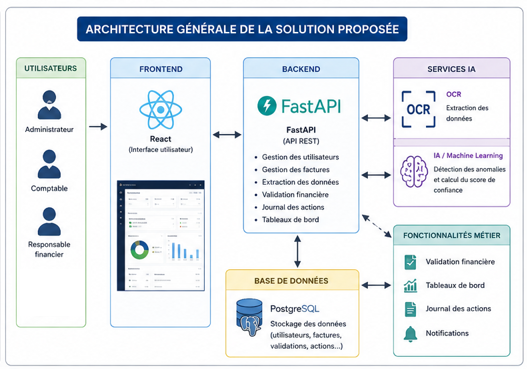
\includegraphics[width=0.6\textwidth]{architecture_generale.jpg}
	\caption{Architecture générale de la solution proposée}
	\label{fig:architecture_generale}
\end{figure}

\FloatBarrier

%====================================================
\section{Méthodologie de travail}
%====================================================

Dans le cadre de ce projet, nous avons étudié deux approches de gestion de projet : les méthodologies classiques et les méthodologies agiles.

Les méthodes classiques reposent sur une organisation séquentielle des phases du projet, tandis que les méthodes agiles offrent plus de flexibilité et permettent une amélioration progressive des fonctionnalités tout au long du développement.

%====================================================
\subsection{Étude comparative}
%====================================================

Avant de choisir la méthodologie adaptée à notre projet, nous avons réalisé une comparaison entre les méthodes traditionnelles et les méthodes agiles afin d’identifier l’approche la plus convenable. Cette comparaison porte sur plusieurs critères tels que le cycle de vie, la planification, la gestion des changements et la livraison des fonctionnalités, comme présenté dans le tableau \ref{tab:comparaison_methodes}.

\begin{table}[H]
	\centering
	\renewcommand{\arraystretch}{1.6}
	
	\begin{tabularx}{\textwidth}{|>{\centering\arraybackslash}m{3.5cm}|X|X|}
		\hline
		
		\rowcolor{gray!25}
		\textbf{Critère} &
		\textbf{Méthodes classiques} &
		\textbf{Méthodes agiles}
		\\ \hline
		
		Cycle de vie &
		Linéaire et séquentiel. &
		Itératif et incrémental.
		\\ \hline
		
		Planification &
		Prévue dès le début. &
		Adaptative et flexible.
		\\ \hline
		
		Documentation &
		Documentation exhaustive. &
		Documentation légère.
		\\ \hline
		
		Organisation &
		Structure hiérarchique. &
		Équipe collaborative.
		\\ \hline
		
		Gestion des changements &
		Changements difficiles à intégrer. &
		Changements intégrés naturellement.
		\\ \hline
		
		Livraison &
		Livraison finale unique. &
		Livraisons progressives.
		\\ \hline
		
		Gestion des risques &
		Détection tardive des risques. &
		Détection rapide des risques.
		\\ \hline
		
	\end{tabularx}
	
	\caption{Comparaison entre les méthodes traditionnelles et agiles}
	\label{tab:comparaison_methodes}
	
\end{table}

Après cette comparaison, nous avons choisi la méthodologie agile car elle permet une meilleure flexibilité, un suivi continu des tâches et une adaptation rapide aux besoins du projet.

Cette approche facilite également la collaboration au sein de l’équipe et la livraison progressive des fonctionnalités.

%====================================================
\subsection{Méthodes agiles}
%====================================================

Les méthodes agiles représentent une approche moderne de gestion de projet basée sur la flexibilité, la collaboration et l’amélioration continue.

Elles permettent de développer les fonctionnalités progressivement tout en s’adaptant rapidement aux changements et aux besoins du client.

Il existe plusieurs méthodologies agiles utilisées dans le domaine du développement logiciel, parmi lesquelles Scrum, Kanban, Extreme Programming (XP) et Lean Software Development.

Ces méthodologies partagent les mêmes principes agiles mais diffèrent dans leur organisation et leurs pratiques de travail.

%====================================================
\subsection{Pourquoi Scrum}
%====================================================

Afin de choisir la méthodologie agile la plus adaptée à notre projet, nous avons réalisé une comparaison entre plusieurs méthodes agiles connues telles que Scrum, Kanban et XP.

Cette comparaison met en évidence les différences au niveau de l’organisation, de la planification, du suivi et des objectifs de chaque méthode, comme présenté dans le tableau \ref{tab:methodes_agiles}.

\begin{table}[H]
	\centering
	\renewcommand{\arraystretch}{1.5}
	
	\begin{tabularx}{\textwidth}{|p{3cm}|X|X|X|}
		\hline
		
		\rowcolor{green!20}
		\textbf{Critère} &
		\textbf{SCRUM} &
		\textbf{Kanban} &
		\textbf{XP}
		\\ \hline
		
		Organisation &
		Travail organisé en sprints. &
		Flux continu. &
		Développement orienté programmation.
		\\ \hline
		
		Planification &
		Sprint planning. &
		Flexible. &
		Flexible.
		\\ \hline
		
		Suivi &
		Réunions quotidiennes. &
		Tableau visuel. &
		Tests fréquents.
		\\ \hline
		
		Objectif &
		Gestion efficace du projet. &
		Optimisation du flux. &
		Qualité du code.
		\\ \hline
		
	\end{tabularx}
	
	\caption{Comparaison entre les méthodes agiles}
	\label{tab:methodes_agiles}
	
\end{table}

%====================================================
\subsection{SCRUM}
%====================================================

La méthodologie SCRUM a été adoptée dans le cadre de ce projet afin d’assurer une gestion agile et efficace des différentes phases de développement.

Cette approche permet d’organiser le travail en plusieurs sprints tout en favorisant la collaboration entre les membres de l’équipe, le suivi continu des tâches et l’amélioration progressive des fonctionnalités développées.

SCRUM repose sur plusieurs éléments essentiels tels que le Product Backlog, qui regroupe l’ensemble des besoins et fonctionnalités du projet, ainsi que le Sprint Backlog qui contient les tâches à réaliser durant chaque sprint.

Chaque sprint possède une durée limitée et se termine par une version fonctionnelle du système.

Cette méthodologie facilite également la communication entre les membres de l’équipe grâce aux réunions régulières appelées Daily Scrum, permettant de suivre l’avancement du projet et de résoudre rapidement les problèmes rencontrés.

De plus, SCRUM offre une grande flexibilité face aux changements et améliore la qualité du produit final grâce aux tests et validations réalisés à chaque sprint. Le cycle de vie de la méthode SCRUM adopté dans notre projet est illustré dans la figure \ref{fig:scrum_cycle}.

\begin{figure}[H]
	\centering
	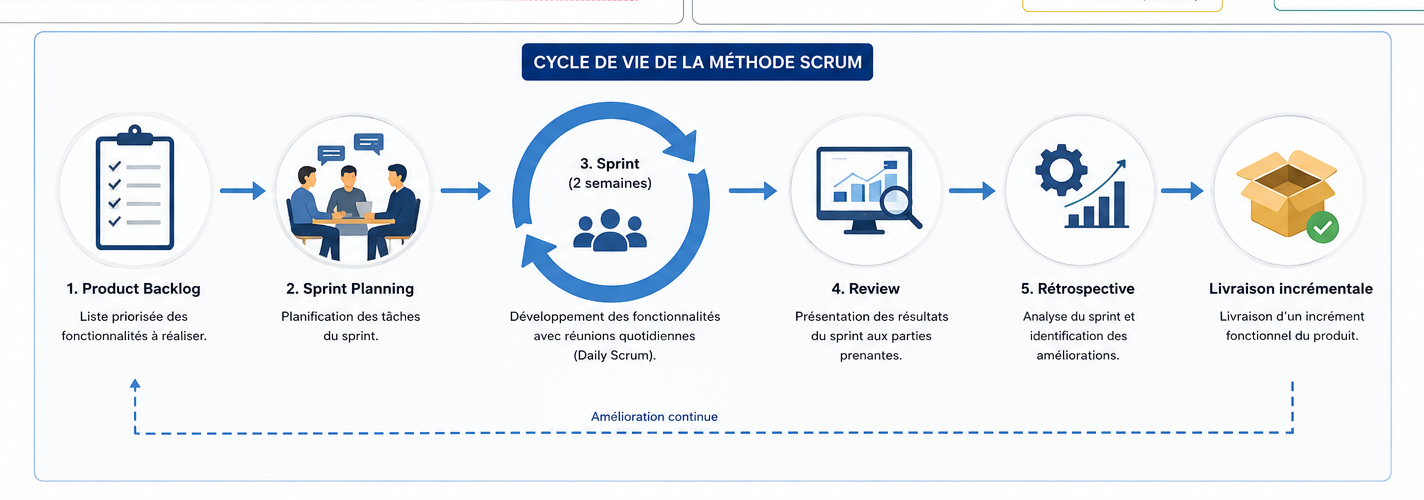
\includegraphics[width=0.7\textwidth]{scrum_cycle.jpg}
	\caption{Cycle de vie de la méthode SCRUM}
	\label{fig:scrum_cycle}
\end{figure}

\FloatBarrier

%====================================================
\section{Langage de modélisation}
%====================================================

Avant de commencer la phase de développement, il est nécessaire de réaliser une étape d’analyse et de conception afin de mieux comprendre le fonctionnement du système et d’organiser les différentes fonctionnalités.

Dans notre projet, nous avons adopté le langage UML (\textit{Unified Modeling Language}) comme outil principal de modélisation. UML permet de représenter graphiquement les besoins fonctionnels, les interactions entre les acteurs ainsi que la structure globale du système. La figure \ref{fig:uml_modelisation} présente les principaux types de diagrammes UML utilisés pour modéliser notre système, notamment les diagrammes de cas d’utilisation, de classes et de séquence.

\begin{figure}[H]
	\centering
	
\includegraphics[width=0.25\textwidth]{uml_modelisation.jpg}
	\caption{Principaux diagrammes UML utilisés}
	\label{fig:uml_modelisation}
\end{figure}



L’utilisation de la modélisation UML offre plusieurs avantages :

\begin{itemize}
	
	\item Faciliter la compréhension du système ;
	
	\item Structurer les fonctionnalités du projet ;
	
	\item Simplifier la communication entre les membres de l’équipe ;
	
	\item Préparer la phase de développement ;
	
	\item Assurer une meilleure organisation des composants du système.
	
\end{itemize}

%====================================================
\section{Conclusion}
%====================================================

Dans ce chapitre, nous avons présenté le cadre général de notre projet à travers une présentation de l’entreprise d’accueil, du contexte général ainsi que de la problématique étudiée. Nous avons également décrit la solution proposée, l’architecture générale du système, la méthodologie de travail adoptée ainsi que le langage de modélisation utilisé durant les phases d’analyse et de conception.
\chapter{Analyse et conception du système}
\newpage
\section{Introduction}

Le deuxième chapitre est consacré à l’analyse et à la conception du système. Nous y présentons les besoins fonctionnels et non fonctionnels, les diagrammes UML ainsi que l’architecture générale de la solution proposée

\section{Identification des acteurs}

\subsection{Comptable} 
Le comptable s’occupe de l’importation des factures dans le système. 
L'utilisateur peut consulter les résultats d’extraction, suivre l’état des factures et vérifier les informations extraites.

\subsection{Responsable financier}

Le responsable financier est chargé d’analyser les factures en attente de décision. 
L'utilisateur peut approuver une facture ou rejeter une facture, et l'utilisateur doit ajouter un commentaire obligatoire pour expliquer la décision.

\subsection{Administrateur}

L’administrateur assure la gestion du système. 
Gérer les utilisateurs, configurer les paramètres de l’intelligence artificielle et consulter le journal des actions permettent de garantir la traçabilité.

\section{Identification des besoins}

\subsection{Besoins fonctionnels}

\begin{table}[H]
	\centering
	\renewcommand{\arraystretch}{1.4}
	
	\begin{tabularx}{\textwidth}{|p{3cm}|c|X|}
		\hline
		\rowcolor{blue!20}
		\textbf{Acteur} & \textbf{ID} & \textbf{Besoin fonctionnel} \\ \hline
		
		\multirow{4}{3cm}{Administrateur}
		& BF1 & Le système doit permettre à l’administrateur de s’authentifier. \\ \cline{2-3}
		& BF2 & Le système doit permettre à l’administrateur de gérer les utilisateurs. \\ \cline{2-3}
		& BF3 & Le système doit permettre à l’administrateur de configurer les seuils de confiance de l’IA. \\ \cline{2-3}
		& BF4 & Le système doit permettre à l’administrateur de consulter le journal des actions. \\ \hline
		
		\multirow{5}{3cm}{Comptable}
		& BF5 & Le système doit permettre au comptable de s’authentifier. \\ \cline{2-3}
		& BF6 & Le système doit permettre au comptable d’importer les factures fournisseurs. \\ \cline{2-3}
		& BF7 & Le système doit extraire automatiquement les données des factures à l’aide de l’OCR. \\ \cline{2-3}
		& BF8 & Le système doit permettre au comptable de consulter les résultats d’extraction. \\ \cline{2-3}
		& BF9 & Le système doit permettre au comptable de gérer les factures selon leurs statuts. \\ \hline
		
		\multirow{3}{3cm}{Responsable financier}
		& BF10 & Le système doit permettre au responsable financier de s’authentifier. \\ \cline{2-3}
		& BF11 & Le système doit permettre au responsable financier d’approuver ou de rejeter les factures avec un commentaire obligatoire. \\ \cline{2-3}
		& BF12 & Le système doit permettre au responsable financier de consulter le tableau de bord financier. \\ \hline
		
	\end{tabularx}
	
	\caption{Besoins fonctionnels du système par acteur}
	\label{tab:besoins_fonctionnels}
\end{table}

\subsection{Besoins non fonctionnels}

Le système doit également respecter les contraintes suivantes :

\begin{itemize}
    \item \textbf{Performance} : traiter les factures rapidement ;
    \item \textbf{Sécurité} : garantir un accès sécurisé grâce à la gestion des rôles ;
    \item \textbf{Fiabilité} : réduire les erreurs qui surviennent pendant le traitement des données ;
    \item \textbf{Ergonomie} : offrir une interface simple à utiliser ;
    \item \textbf{Scalabilité} : faciliter la gestion d’un grand nombre de factures ;
    \item \textbf{Disponibilité} : Disponibilité signifie que le système reste accessible à tout moment ;
    \item \textbf{Traçabilité} : enregistrer les actions du système.
\end{itemize}

\section{Diagramme de cas d’utilisation global}

Le diagramme de cas d’utilisation global présente les interactions entre les différents acteurs du système, à savoir le comptable, le responsable financier et l’administrateur. 
Il permet de visualiser les principales fonctionnalités offertes par la plateforme.

\begin{figure}[H]
\centering
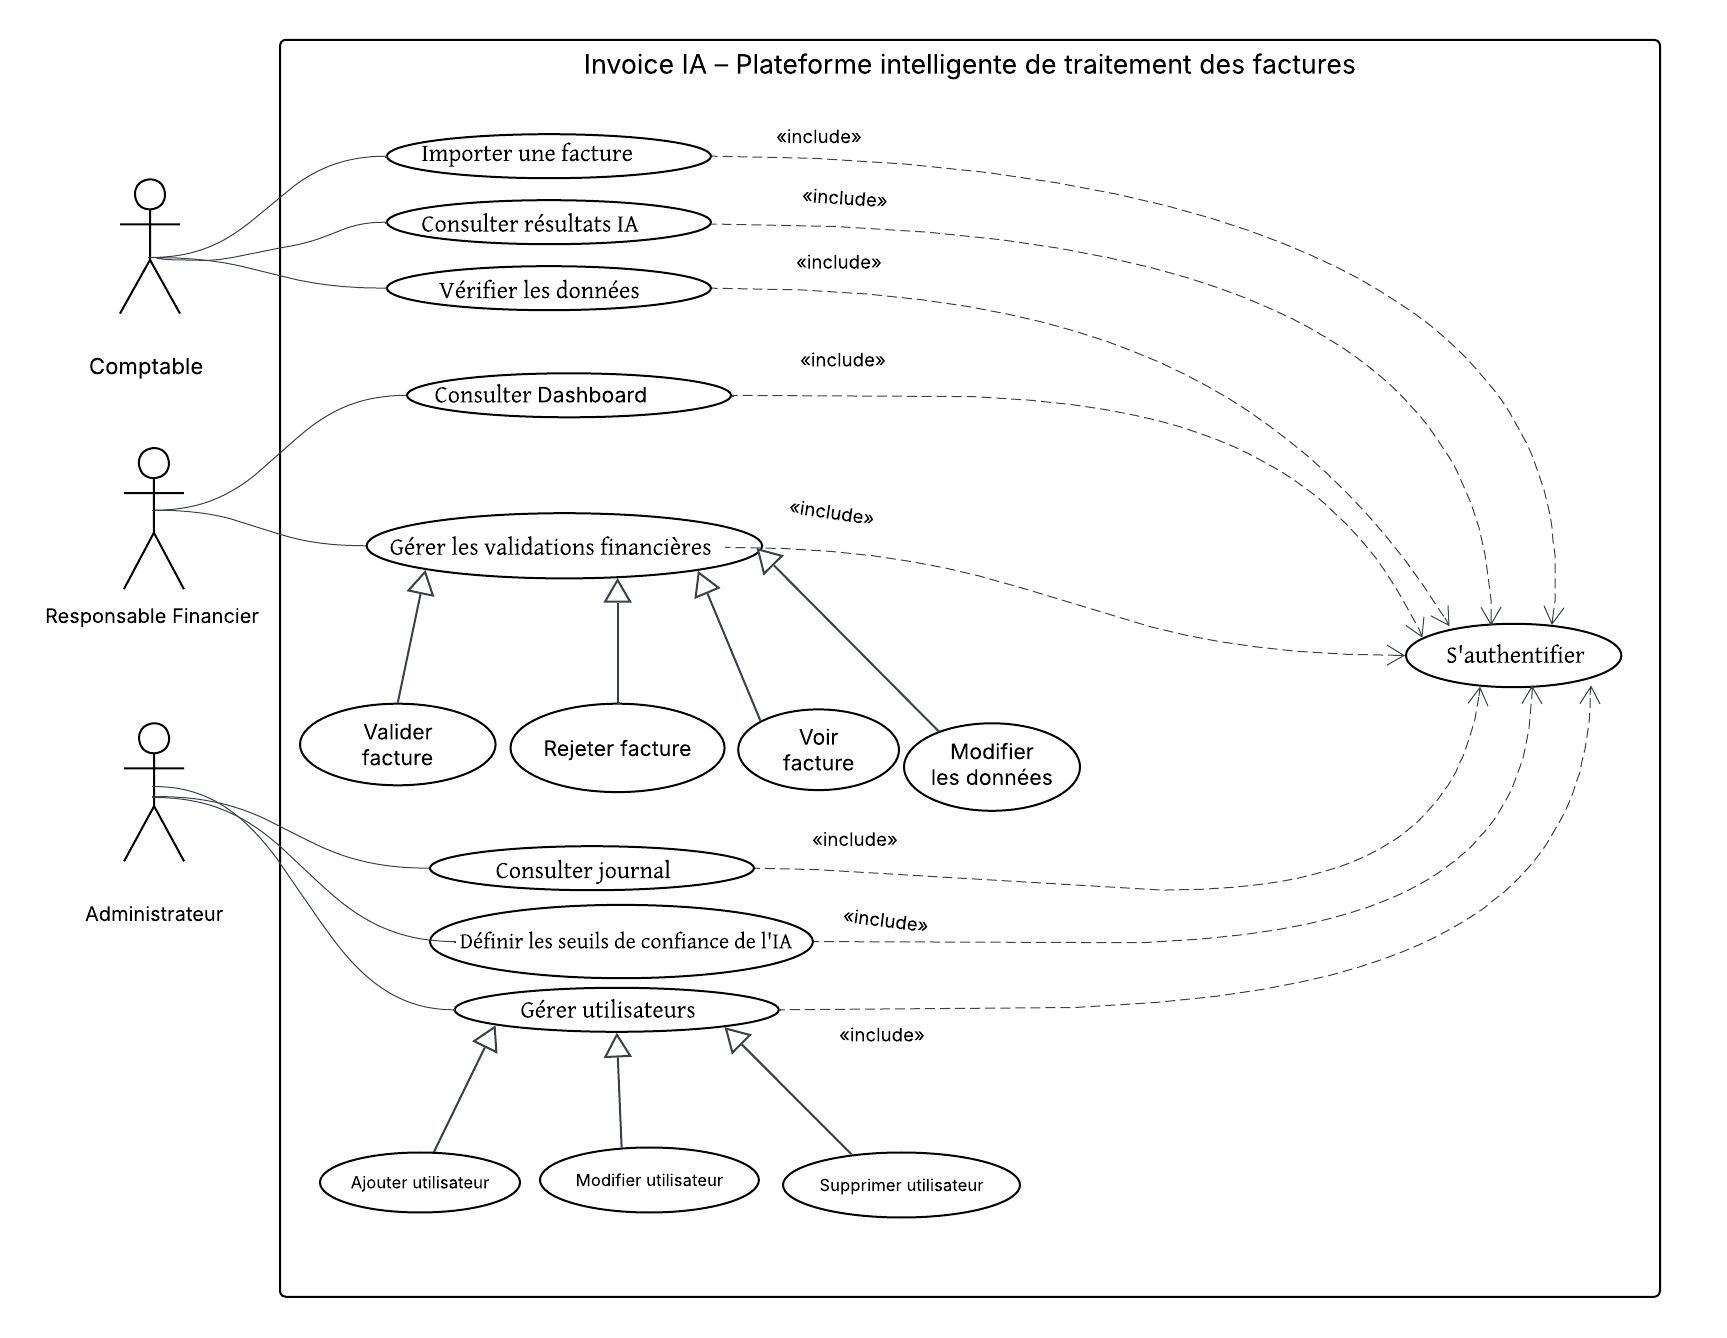
\includegraphics[width=1.0\textwidth]{usecase.jpg}
\caption{Diagramme de cas d’utilisation global du système}
\label{fig:usecase_global}
\end{figure}

\FloatBarrier
\section{Diagramme de classes global}

Le diagramme de classes global ci-dessous illustre la structure de la solution Inovoice IA. Il présente les entités du système, leurs attributs ainsi que les relations entre les différents acteurs et composants.
\begin{figure}[H]
	\centering
	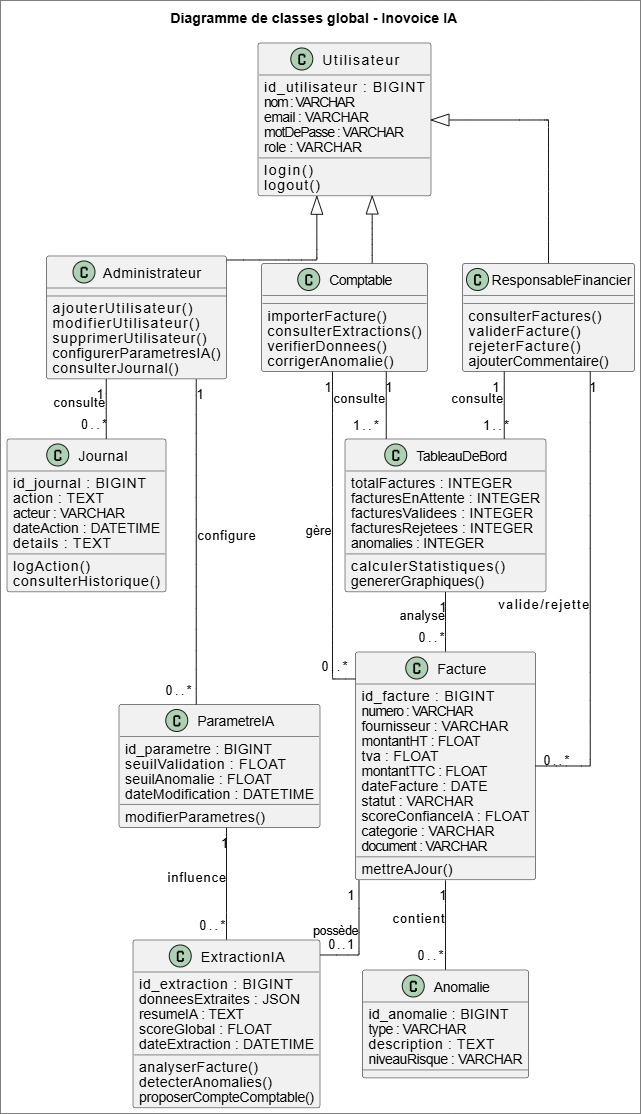
\includegraphics[width=0.8\textwidth]{diagramme_classes_global.jpg}
	\caption{Diagramme de classes global du système}
	\label{fig:diagramme_classes_global}
\end{figure}

\FloatBarrier
\section{Architecture du travail}

\subsection{Architecture physique : Architecture 3-tiers }


L’architecture physique du système repose sur une architecture 3-tiers\cite{architecture3tiers} permettant de séparer l’interface utilisateur, la logique métier et la base de données. Cette organisation facilite la maintenance, la sécurité et l’évolution du système.

Notre architecture est composée des éléments suivants :

\begin{itemize}
	
	\item \textbf{Frontend :} représente l’interface utilisateur développée avec React.
	
	\item \textbf{Backend :} assure la logique métier et la gestion des requêtes via FastAPI.
	
	\item \textbf{Base de données :} PostgreSQL permet le stockage des utilisateurs, factures et validations.
	
	\item \textbf{Services OCR/IA :} utilisés pour l’extraction et l’analyse automatique des données.
	
	\item \textbf{Workflow n8n :} permet l’automatisation des traitements et des processus du système.
	
\end{itemize}
Comme présenté dans la figure
\ref{fig:architecture_physique}.
\begin{figure}[H]
\centering
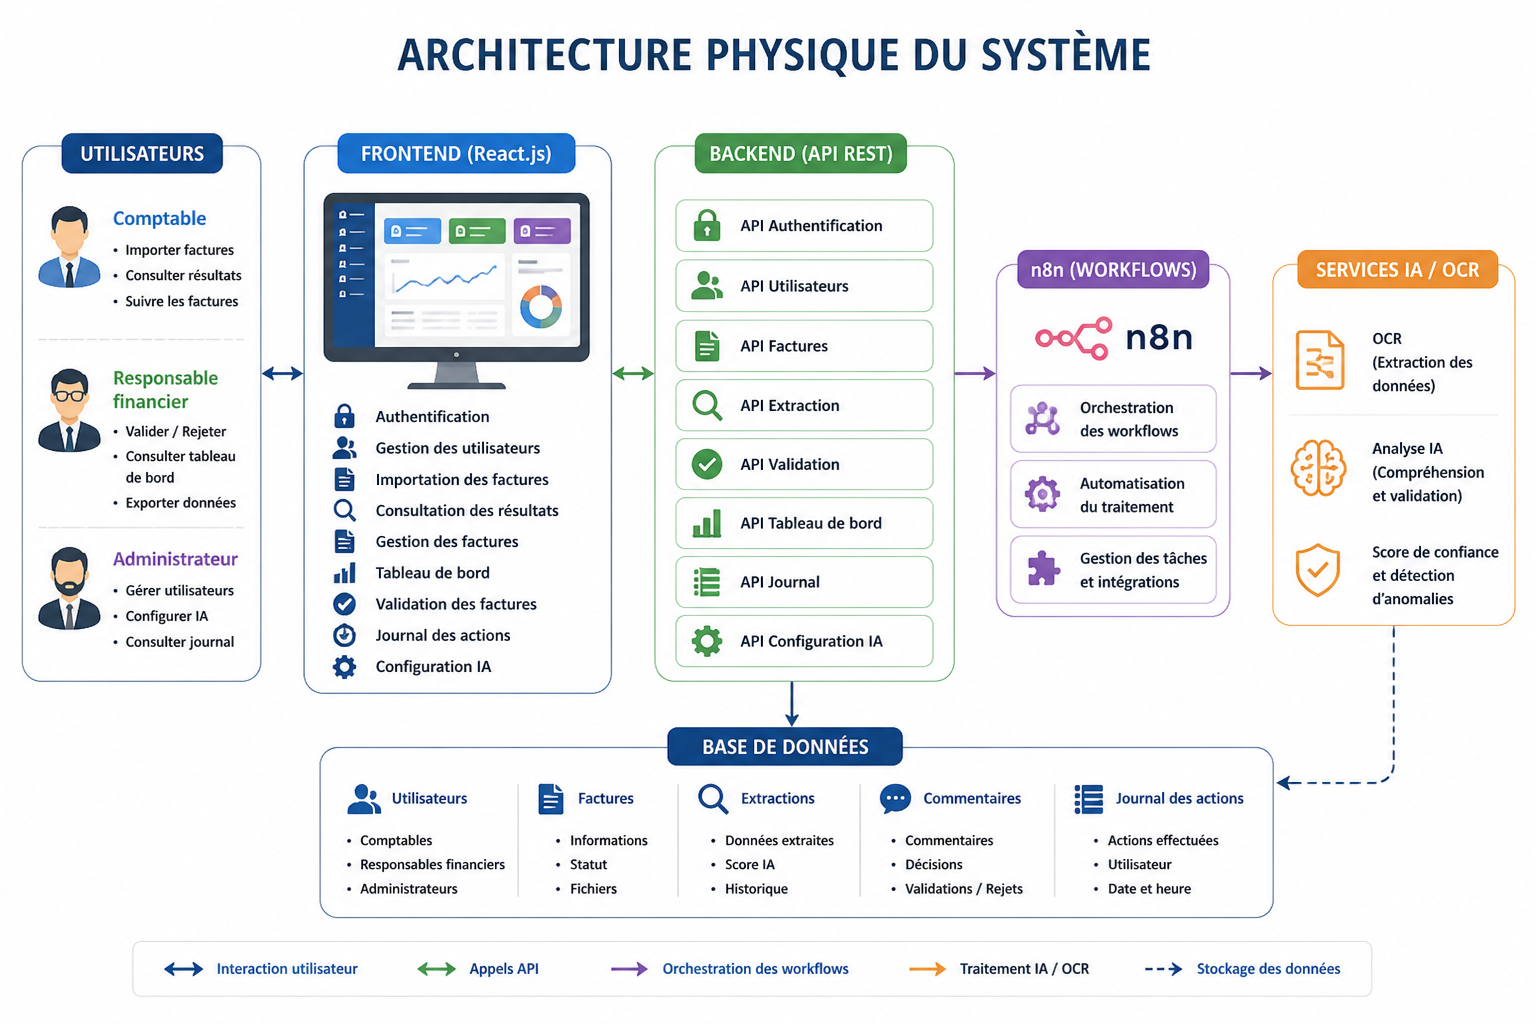
\includegraphics[width=1.0\textwidth]{architecture_physique.jpg}
\caption{Architecture physique du système}
\label{fig:architecture_physique}
\end{figure}

\FloatBarrier

\subsection{Architecture logique : MVC}
L’architecture logique du système s’appuie sur plusieurs couches ; ces couches assurent la clarté et la modularité du système.

Cette architecture logique repose également sur le modèle \textbf{MVC}, où le frontend représente la couche \textbf{View}, le backend représente la couche \textbf{Controller} et la base de données correspond à la couche \textbf{Model}.


\begin{itemize}
    \item \textbf{Présentation (Frontend)} : La Présentation (Frontend) gère l'interface utilisateur ainsi que les interactions ;
    \item \textbf{Contrôle (Backend)} : assure la logique métier et les traitements ;
    \item \textbf{Données (Base de données)} : Données (Base de données) assure le stockage des informations ;
    \item \textbf{Workflow (n8n)} : gère les traitements automatisés ;
    \item \textbf{Services IA / OCR} : Les Services IA / OCR permettent d’extraire et d’analyser les données.
\end{itemize}
Comme présenté dans la figure
\ref{fig:architecture_logique}.
\begin{figure}[H]
\centering
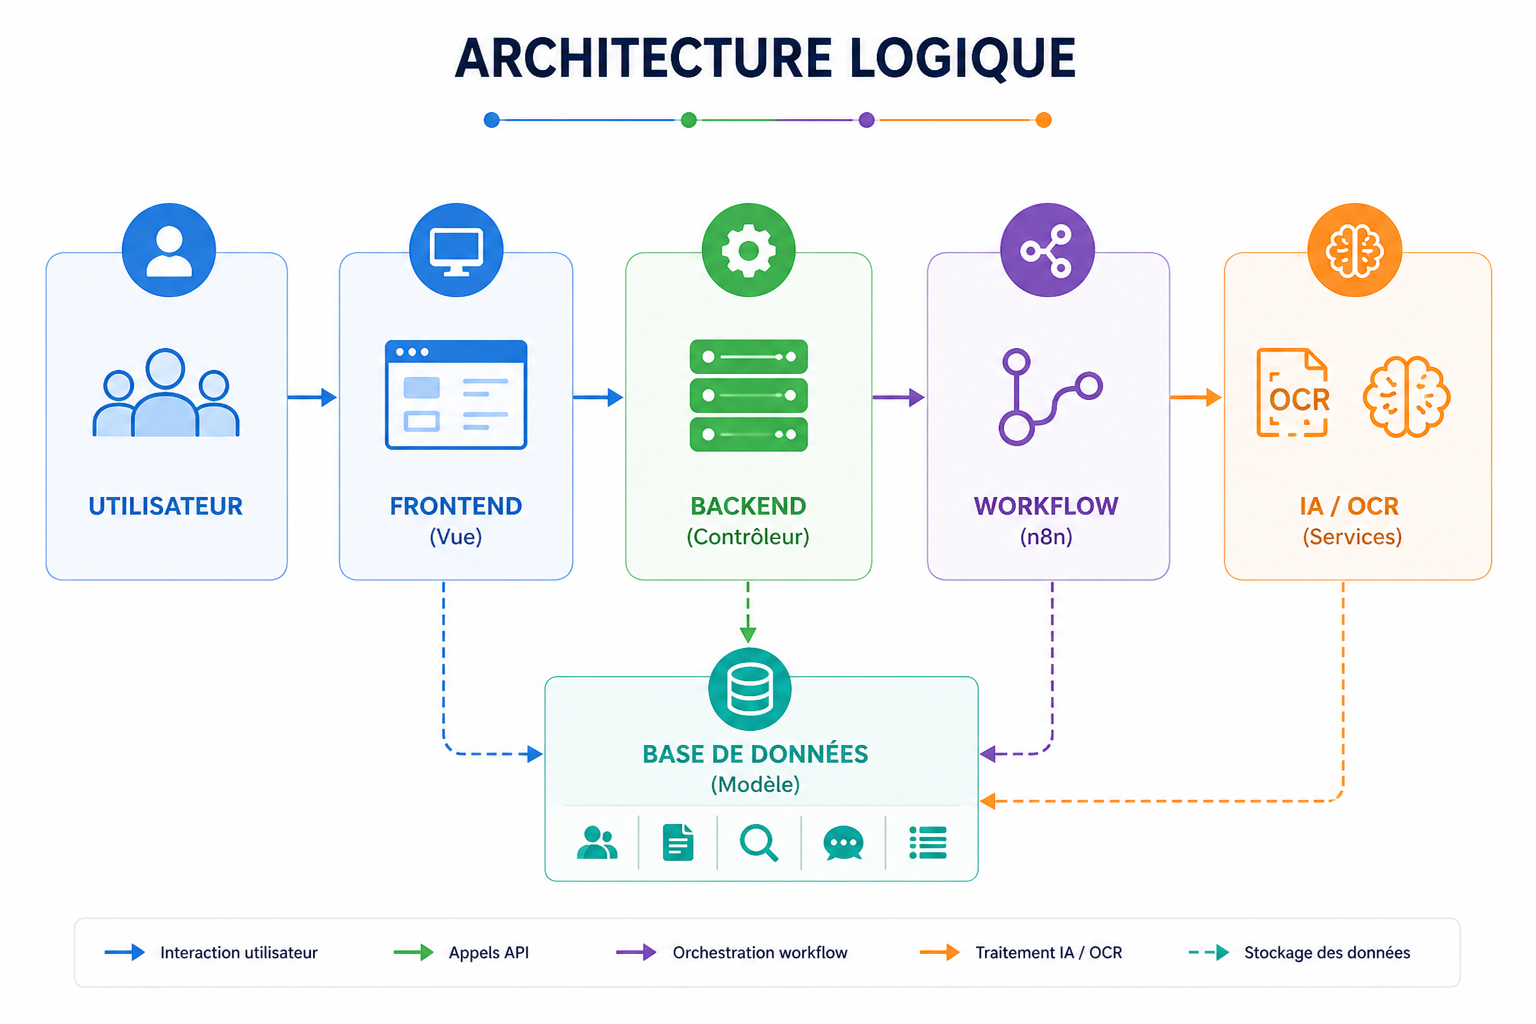
\includegraphics[width=1.0\textwidth]{architecture_logique.jpg}
\caption{Architecture logique du système}
\label{fig:architecture_logique}
\end{figure}

\FloatBarrier

\subsection{Pilotage avec Scrum}

Dans le cadre de notre projet, nous avons adopté la méthodologie Agile Scrum. 
Cette méthode permet d’organiser le travail en plusieurs itérations appelées sprints. 
Chaque sprint regroupe un ensemble de fonctionnalités. Le sprint développe les fonctionnalités, teste les fonctionnalités et valide les fonctionnalités.

\subsubsection{Répartition des rôles}

L’équipe Scrum comprend les rôles suivants :



\begin{itemize}
    \item \textbf{Product Owner} : Product Owner définit les besoins et gère le backlog produit ;
    \item \textbf{Scrum Master} : Scrum Master veille à ce que le projet se passe bien et facilite le travail de l’équipe ;
    \item \textbf{Équipe de développement} : Équipe de développement conçoit, développe et teste l’application.
\end{itemize}
Comme présenté dans la figure
\ref{fig:scrum_team}.
\begin{figure}[H]
\centering
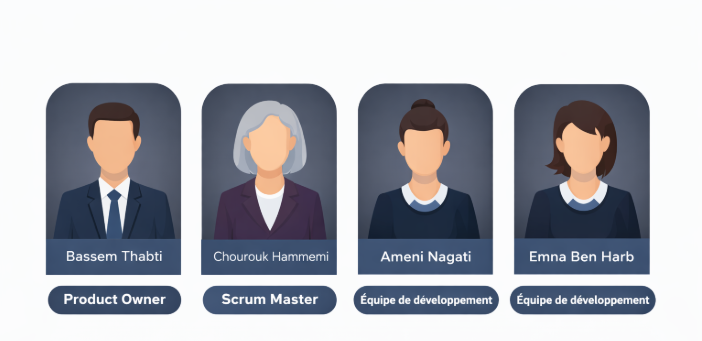
\includegraphics[width=0.85\textwidth]{scrum_team.jpg}
\caption{Organisation de l’équipe Scrum}
\label{fig:scrum_team}
\end{figure}

\FloatBarrier

\subsubsection{Backlog produit}

Le backlog produit regroupe l’ensemble des fonctionnalités à développer dans le système.
Les fonctionnalités sont présentées sous forme de user stories.
Comme présenté dans le tableau \ref{tab:product_backlog}.
\begin{table}[H]
\centering
\small
\renewcommand{\arraystretch}{1.35}
\setlength{\tabcolsep}{4pt}

\begin{tabularx}{\textwidth}{|p{3cm}|c|X|X|}
\hline
\rowcolor{blue!20}
\textbf{Acteur} & \textbf{ID} & \textbf{User Story} & \textbf{Description} \\
\hline

\multirow{4}{3cm}{Administrateur}
& 1 & En tant qu’administrateur, je veux gérer les utilisateurs afin de contrôler l’accès au système. 
& Ajouter, modifier ou supprimer les utilisateurs. \\ \cline{2-4}

& 2 & En tant qu’administrateur, je veux configurer les seuils IA afin d’adapter le traitement automatique. 
& Définir les seuils de confiance de l’intelligence artificielle. \\ \cline{2-4}

& 3 & En tant qu’administrateur, je veux consulter le journal des actions afin d’assurer la traçabilité. 
& Afficher l’historique des actions du système. \\ \cline{2-4}

& 4 & En tant qu’administrateur, je veux sécuriser l’accès afin de protéger le système. 
& Assurer l’authentification et la gestion des rôles. \\
\hline

\multirow{5}{3cm}{Comptable}
& 5 & En tant que comptable, je veux importer une facture afin de lancer son traitement. 
& Importer une facture au format PDF ou image. \\ \cline{2-4}

& 6 & En tant que comptable, je veux extraire automatiquement les données afin de réduire la saisie manuelle. 
& Extraire les données des factures avec l’OCR et l’IA. \\ \cline{2-4}

& 7 & En tant que comptable, je veux consulter les résultats d’extraction afin de vérifier les données. 
& Afficher les résultats d’extraction. \\ \cline{2-4}

& 8 & En tant que comptable, je veux gérer les factures selon leurs statuts afin de suivre leur état. 
& Consulter les factures en attente, validées et avec anomalies. \\ \cline{2-4}

& 9 & En tant que comptable, je veux consulter le tableau de bord afin de suivre les indicateurs. 
& Afficher les statistiques des factures. \\
\hline

\multirow{3}{3cm}{Responsable financier}
& 10 & En tant que responsable financier, je veux approuver une facture avec un commentaire afin de justifier ma décision. 
& Approuver une facture après analyse. \\ \cline{2-4}

& 11 & En tant que responsable financier, je veux rejeter une facture avec un commentaire afin de signaler une anomalie. 
& Rejeter une facture avec une justification obligatoire. \\ \cline{2-4}

& 12 & En tant que responsable financier, je veux consulter le tableau de bord financier et exporter les données. 
& Visualiser les indicateurs financiers et exporter les données. \\
\hline

\end{tabularx}

\caption{Product Backlog du système}
\label{tab:product_backlog}
\end{table}



\FloatBarrier
\newpage
\section{Planification des sprints}

Le projet est réparti en trois sprints afin d’assurer une progression logique et cohérente du développement.

Comme présenté dans la figure \ref{fig:planification_sprints}.

\begin{figure}[H]
\centering
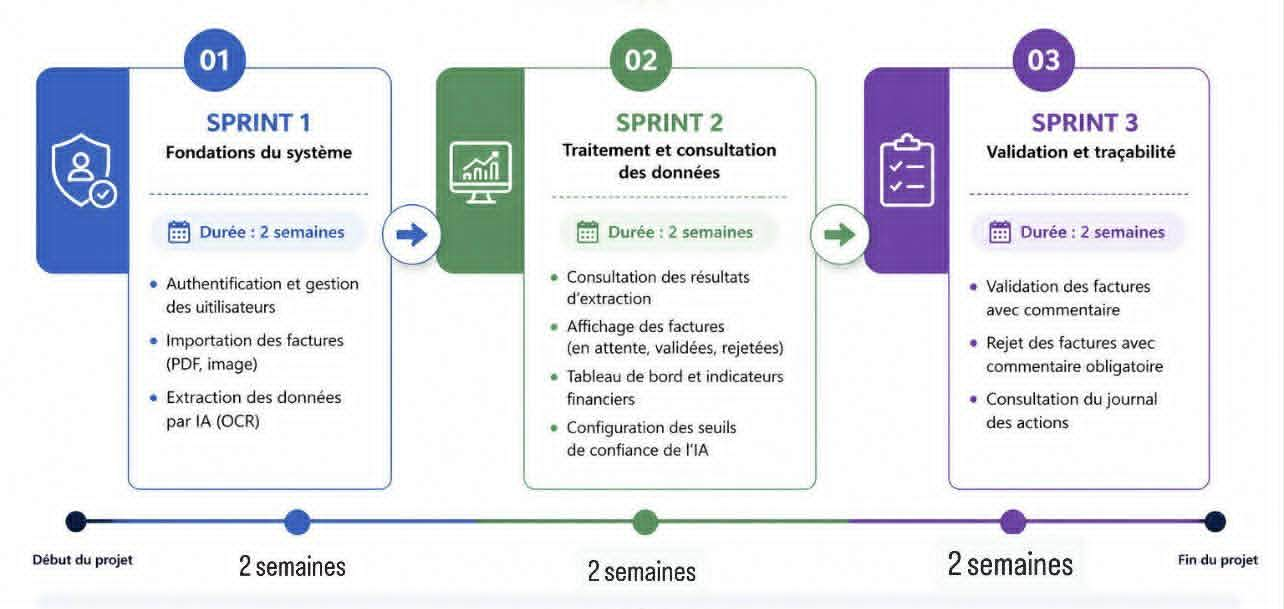
\includegraphics[width=1.0\textwidth]{planification_sprints.jpg}
\caption{Planification des sprints du projet}
\label{fig:planification_sprints}
\end{figure}

\FloatBarrier

\section{Environnement de travail}

Dans cette section, nous présentons les équipements matériels et les outils logiciels utilisés pour la réalisation du projet.

\subsection{Environnement matériel}

La réalisation de ce projet a été effectuée en utilisant deux machines ayant les caractéristiques suivantes :

\begin{table}[H]
\centering
\caption{Environnement matériel}
\begin{tabular}{|l|c|c|}
\hline
\textbf{Caractéristique} & \textbf{PC 1} & \textbf{PC 2} \\
\hline
Système d’exploitation & Windows 10 & Windows 11 \\
\hline
Processeur & Intel Core i5 & Intel Core i5-9300H \\
\hline
Mémoire RAM & 16 Go & 16 Go \\
\hline
Disque dur & 512 Go (SSD) & 251 Go (SSD) \\
\hline
\end{tabular}
\end{table}

\FloatBarrier
\newpage
\subsection{Environnement logiciel}

\renewcommand{\arraystretch}{2.3}

\begin{longtable}{|m{3cm}|m{3.5cm}|m{8cm}|}
	\hline
	
	\rowcolor{blue!25}
	\centering \textbf{Logo} &
	\centering \textbf{Outil} &
	\centering \textbf{Description}
	\tabularnewline
	\hline
	
	\endfirsthead
	
	\hline
	\rowcolor{blue!25}
	\centering \textbf{Logo} &
	\centering \textbf{Outil} &
	\centering \textbf{Description}
	\tabularnewline
	\hline
	
	\endhead
	
	\centering 
\includegraphics[width=2.5cm]{figures/logos/staruml.jpg}
	&
	\centering \textbf{Star UML}
	&
	Outil de modélisation UML utilisé pour concevoir les différents diagrammes du projet, notamment les diagrammes de cas d’utilisation, de séquence et de classes, facilitant ainsi l’analyse et la conception du système \cite{online:staruml}.
	\tabularnewline
	\hline
	
	\centering 
\includegraphics[width=2.5cm]{figures/logos/react.jpg}
	&
	\centering \textbf{React}
	&
	Bibliothèque JavaScript utilisée pour développer une interface utilisateur moderne, dynamique et interactive, garantissant une meilleure expérience utilisateur et une navigation fluide au sein de la plateforme \cite{online:react}.
	\tabularnewline
	\hline
	
	\centering 
\includegraphics[width=2.5cm]{figures/logos/fastapi.jpg}
	&
	\centering \textbf{FastAPI}
	&
	Framework Python utilisé pour le développement du backend du système, permettant la création d’API REST performantes, sécurisées et rapides pour assurer la communication entre les différentes composantes du projet \cite{online:fastapi}.
	\tabularnewline
	\hline
	
	\centering 
\includegraphics[width=2.5cm]{figures/logos/n8n.jpg}
	&
	\centering \textbf{n8n}
	&
	Plateforme d’automatisation utilisée pour orchestrer les workflows et automatiser les traitements liés à l’importation, l’analyse et la validation des factures dans le système \cite{online:n8n}.
	\tabularnewline
	\hline
	
	\centering 
\includegraphics[width=2.5cm]{figures/logos/ocr.jpg}
	&
	\centering \textbf{OCR / IA}
	&
	Technologies utilisées pour extraire automatiquement les données des factures fournisseurs, analyser leur contenu et attribuer des scores de confiance grâce aux mécanismes d’intelligence artificielle \cite{ocr}.
	\tabularnewline
	\hline
	
	\centering 
\includegraphics[width=2.5cm]{figures/logos/postgresql.jpg}
	&
	\centering \textbf{PostgreSQL}
	&
	Système de gestion de base de données relationnelle utilisé pour stocker les données du système de manière fiable, sécurisée et performante \cite{online:postgresql}.
	\tabularnewline
	\hline
	
	\centering 
\includegraphics[width=2.5cm]{figures/logos/pgadmin.jpg}
	&
	\centering \textbf{pgAdmin}
	&
	Interface graphique utilisée pour administrer la base de données PostgreSQL, gérer les tables, exécuter les requêtes SQL et superviser les données du système \cite{online:pgadmin}.
	\tabularnewline
	\hline

	
	\centering 
\includegraphics[width=2.5cm]{figures/logos/postman.jpg}
	&
	\centering \textbf{Postman}
	&
	Outil de test utilisé pour vérifier le bon fonctionnement des API REST développées, envoyer des requêtes HTTP et analyser les réponses retournées par le backend \cite{online:postman}.
	\tabularnewline
	\hline
	
	\centering 
\includegraphics[width=2.5cm]{figures/logos/vscode.jpg}
	&
	\centering \textbf{Visual Studio Code}
	&
	Environnement de développement utilisé pour écrire, organiser, maintenir et tester le code source du frontend et du backend du projet \cite{online:vscode}.
	\tabularnewline
	\hline
	
\end{longtable}



\newpage
\section{Diagramme de Gantt}

Le diagramme de Gantt permet de représenter la planification temporelle des différentes tâches du projet. 
Il donne une vision globale de l’enchaînement des sprints et de la durée prévue pour chaque étape.
Comme présenté dans la figure \ref{fig:gantt}.
\begin{figure}[H]
\centering
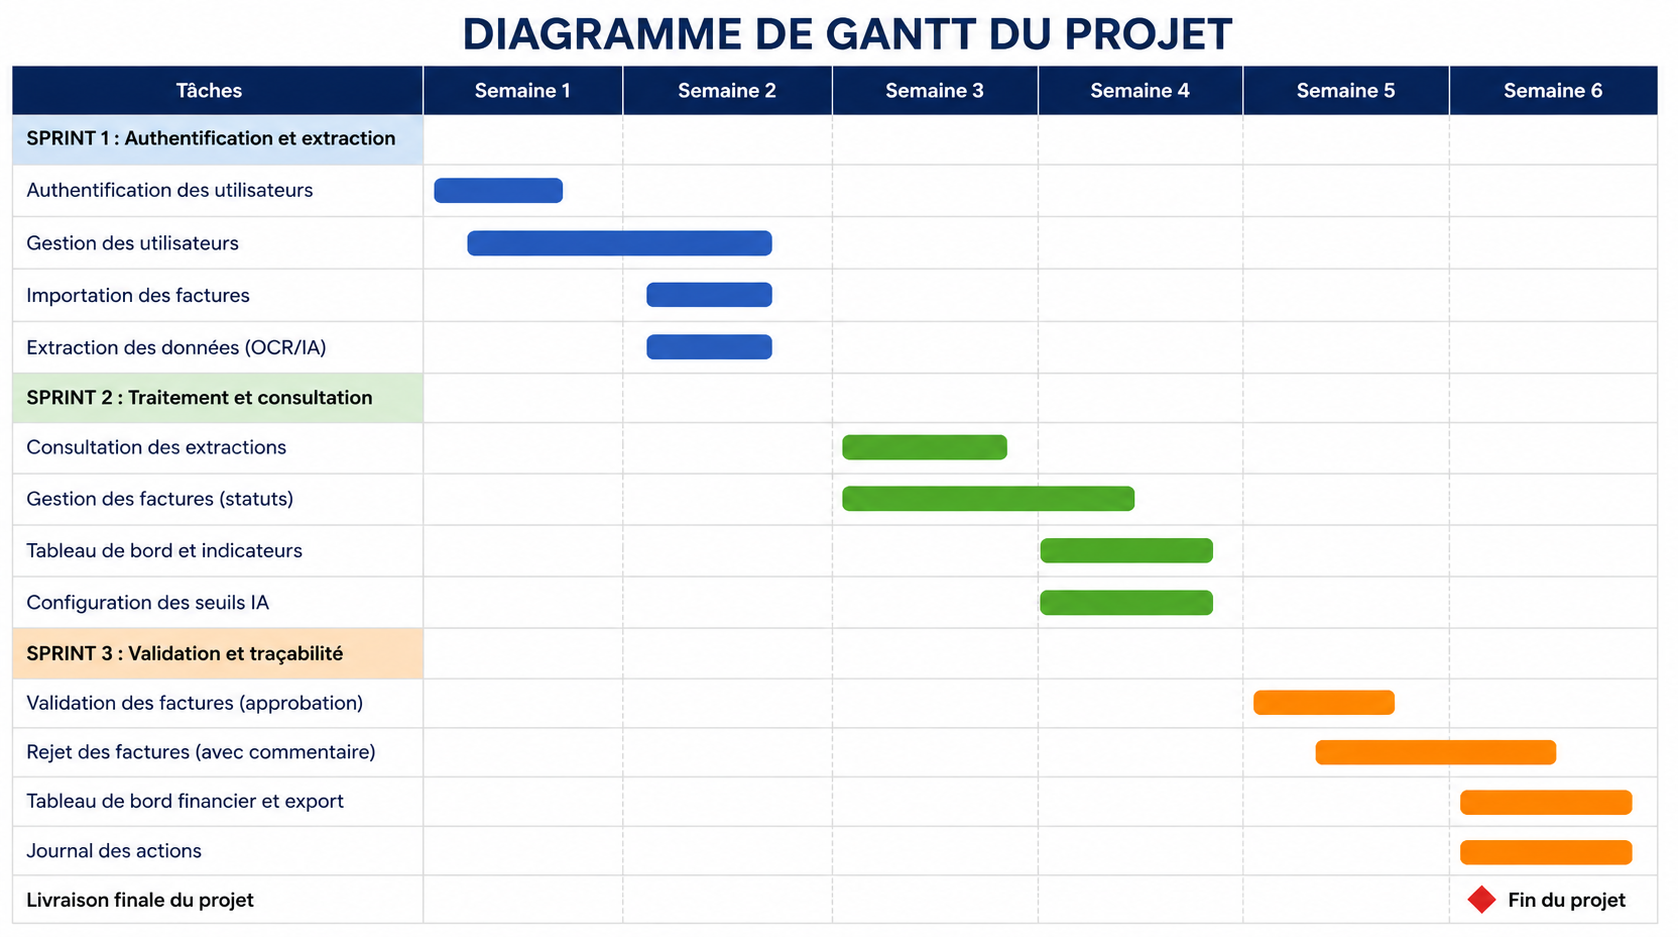
\includegraphics[width=1.0\textwidth]{gantt.jpg}
\caption{Diagramme de Gantt du projet}
\label{fig:gantt}
\end{figure}

\FloatBarrier

\section*{Conclusion}

Dans ce chapitre, nous avons présenté l’analyse et la conception du système. Nous avons défini les besoins fonctionnels et non fonctionnels, puis élaboré les différents diagrammes UML ainsi que l’architecture générale de la solution proposée.
\chapter{Sprint 1 : Authentification et gestion des utilisateurs}


\newpage

\section{Introduction}

Le troisième chapitre présente les réalisations du Sprint 1. Nous détaillons les fonctionnalités liées à l’authentification, à la gestion des utilisateurs ainsi qu’à l’importation et l’extraction des données des factures.

\section{Backlog du Sprint}

\renewcommand{\arraystretch}{1.5}

\begin{table}[H]
	\centering
	\small
	\begin{tabularx}{\textwidth}{|c|p{3.8cm}|c|p{6cm}|c|}
		\hline
		\rowcolor{blue!20}
		\textbf{ID} & \textbf{User Story} & \textbf{ID-US} & \textbf{Tâche} & \textbf{Estimation} \\ \hline
		
		\multirow{4}{*}{1.1}
		& \multirow{4}{3.8cm}{En tant qu’utilisateur, je veux m’authentifier afin d’accéder au système.}
		& 1.1.1 & Conception des diagrammes UML. & \multirow{4}{*}{1 jour} \\ \cline{3-4}
		& & 1.1.2 & Développement de l’interface de connexion. & \\ \cline{3-4}
		& & 1.1.3 & Implémentation de l’API d’authentification. & \\ \cline{3-4}
		& & 1.1.4 & Tests et validation. & \\ \hline
		
		\multirow{4}{*}{1.2}
		& \multirow{4}{3.8cm}{En tant qu’administrateur, je veux gérer les utilisateurs afin de contrôler les accès.}
		& 1.2.1 & Conception UML de la gestion des utilisateurs. & \multirow{4}{*}{2 jours} \\ \cline{3-4}
		& & 1.2.2 & Développement des interfaces CRUD utilisateurs. & \\ \cline{3-4}
		& & 1.2.3 & Implémentation backend CRUD utilisateurs. & \\ \cline{3-4}
		& & 1.2.4 & Tests et validation. & \\ \hline
		
		\multirow{4}{*}{1.3}
		& \multirow{4}{3.8cm}{En tant que comptable, je veux importer une facture afin de lancer son traitement.}
		& 1.3.1 & Conception du processus d’importation. & \multirow{4}{*}{2 jours} \\ \cline{3-4}
		& & 1.3.2 & Développement de l’interface d’importation. & \\ \cline{3-4}
		& & 1.3.3 & Intégration de l’API d’importation. & \\ \cline{3-4}
		& & 1.3.4 & Tests d’importation. & \\ \hline
		
		\multirow{4}{*}{1.4}
		& \multirow{4}{3.8cm}{En tant que comptable, je veux extraire les données des factures via OCR/IA.}
		& 1.4.1 & Intégration du service OCR/IA. & \multirow{4}{*}{3 jours} \\ \cline{3-4}
		& & 1.4.2 & Traitement des données extraites. & \\ \cline{3-4}
		& & 1.4.3 & Stockage des résultats en base. & \\ \cline{3-4}
		& & 1.4.4 & Tests et validation. & \\ \hline
		
	\end{tabularx}
	\caption{Backlog détaillé du Sprint 1}
	\label{tab:backlog_sprint1}
\end{table}

\FloatBarrier

\section{Analyse}

\subsection{Analyse fonctionnelle}

\subsubsection{Diagramme de cas d’utilisation}

Le diagramme de cas d’utilisation montre clairement les fonctions principales du
premier sprint. Le diagramme de cas d’utilisation met en avant les interactions entre
les acteurs et le système, notamment l’authentification, la gestion des utilisateurs,
l’importation des factures et l’extraction des données.

\begin{figure}[H]
	\centering
	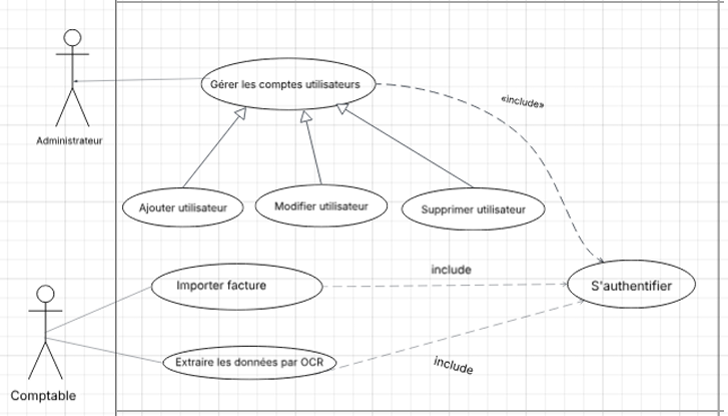
\includegraphics[width=0.9\textwidth]{usecase_sprint1.jpg}
	\caption{Diagramme de cas d’utilisation du Sprint 1}
	\label{fig:usecase_sprint1}
\end{figure}
\subsubsection{Description textuelle des cas d’utilisation}

\subsubsection*{Cas d’utilisation : S’authentifier}

\begin{table}[H]
	\centering
	\renewcommand{\arraystretch}{1.35}
	\rowcolors{2}{gray!10}{white}
	
	\begin{tabularx}{\textwidth}{|p{2.8cm}|X|}
		\hline
		\rowcolor{blue!20}
		\textbf{Use Case} & S’authentifier \\ \hline
		
		\textbf{Acteur} & Utilisateur \\ \hline
		
		\textbf{Description} & Permet à l’utilisateur d’accéder au système de manière sécurisée à l’aide de ses identifiants. \\ \hline
		
		\textbf{Pré-condition} & La page de connexion est affichée. \\ \hline
		
		\rowcolor{blue!10}
		\textbf{Scénario nominal} &
		1- L’utilisateur entre l’adresse e-mail et le mot de passe. \newline
		2- Le système contrôle que les informations saisies sont valides. \newline
		3- Le système identifie le rôle de l’utilisateur. \newline
		4- Le système permet l’accès et envoie l’utilisateur à son interface principale. \\ \hline
		
		\textbf{Post-condition} & L’utilisateur est authentifié et accède à son espace. \\ \hline
		
		\rowcolor{blue!10}
		\textbf{Scénarios alternatifs} &
		1- Champs vides. \newline
		1.1- Le système montre un message d’erreur. \newline
		2- Les identifiants sont incorrects. \newline
		2.1- Le système refuse l’accès. \\ \hline
		
	\end{tabularx}
	
	\caption{Description textuelle du cas d’utilisation « S’authentifier »}
	\label{tab:authentification}
\end{table}



\subsubsection*{Cas d’utilisation : Gérer les utilisateurs}

\begin{table}[H]
	\centering
	\renewcommand{\arraystretch}{1.5}
	\small
	
	\begin{tabularx}{\textwidth}{|p{4.5cm}|X|}
		\hline
		\rowcolor{blue!20}
		\textbf{Nom du cas d’utilisation}
		& Gérer les utilisateurs \\ \hline
		
		\textbf{Description brève}
		& L’administrateur ajoute, modifie ou supprime les utilisateurs du système. \\ \hline
		
		\textbf{Acteurs primaires}
		& Administrateur \\ \hline
		
		\textbf{Acteurs secondaires}
		& Aucun \\ \hline
		
		\textbf{Pré-condition}
		& L’administrateur doit être authentifié. \\ \hline
		
		\textbf{Scénario nominal}
		&
		1- Le cas d’utilisation commence dès que l’administrateur ouvre l’interface de gestion des utilisateurs. \newline
		2- Le système affiche la liste des utilisateurs. Il indique les actions disponibles. \newline
		3- Si l’administrateur clique sur « Ajouter » : \newline
		\hspace*{0.5cm}3.1- Le système montre le formulaire d’ajout. \newline
		\hspace*{0.5cm}3.2- L’administrateur entre les données du nouvel utilisateur. \newline
		\hspace*{0.5cm}3.3- Le système contrôle les données saisies, le système garantit la cohérence. \newline
		\hspace*{0.5cm}3.4- Le système enregistre l’utilisateur. \newline
		\hspace*{0.5cm}3.5- Le système affiche un message de confirmation. \newline
		4- Si l’administrateur sélectionne « Modifier » : \newline
		\hspace*{0.5cm}4.1- Le système montre les informations de l’utilisateur sélectionné. \newline
		\hspace*{0.5cm}4.2- L’administrateur modifie les données voulues. \newline
		\hspace*{0.5cm}4.3- Le système enregistre les modifications. \newline
		\hspace*{0.5cm}4.4- Le système montre un message de confirmation. \newline
		5- Si l’administrateur sélectionne « Supprimer » : \newline
		\hspace*{0.5cm}5.1- Le système demande à l’utilisateur de confirmer. \newline
		\hspace*{0.5cm}5.2- L’administrateur confirme la suppression. \newline
		\hspace*{0.5cm}5.3- Le système supprime l’utilisateur. \newline
		\hspace*{0.5cm}5.4- Le système montre un message de confirmation. \\ \hline
		
		\textbf{Post-condition}
		& Les informations des utilisateurs sont mises à jour dans le système. \\ \hline
		
		\textbf{Scénarios alternatifs}
		&
		1- Informations invalides ou incomplètes. \newline
		1.1- Le système affiche un message d’erreur. \newline
		2- Adresse email déjà utilisée. \newline
		2.1- Le système refuse l’enregistrement. \newline
		3- Utilisateur introuvable. \newline
		3.1- Le système annule l’opération. \\ \hline
		
	\end{tabularx}
	
	\caption{Description textuelle du cas d’utilisation « Gérer les utilisateurs »}
	\label{tab:gerer_utilisateurs}
\end{table}

\FloatBarrier

\subsection{Analyse dynamique}

\subsubsection{Diagramme de séquence système du cas d’utilisation « S’authentifier »}

Le diagramme de séquence du système montre les échanges entre l’utilisateur et le système pendant l’authentification. Le diagramme décrit le déroulement de l’authentification.

\begin{figure}[H]
	\centering
	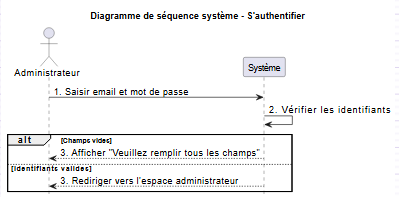
\includegraphics[width=0.85\textwidth]{seq_auth.jpg}
	\caption{Diagramme de séquence système du cas d’utilisation « S’authentifier »}
	\label{fig:seq_auth}
\end{figure}

\FloatBarrier

\subsubsection{Diagramme de séquence système du cas d’utilisation « Gérer les utilisateurs »}

Le diagramme de séquence du système montre comment l’administrateur interagit avec le système lors de la gestion des utilisateurs.

\begin{figure}[H]
	\centering
	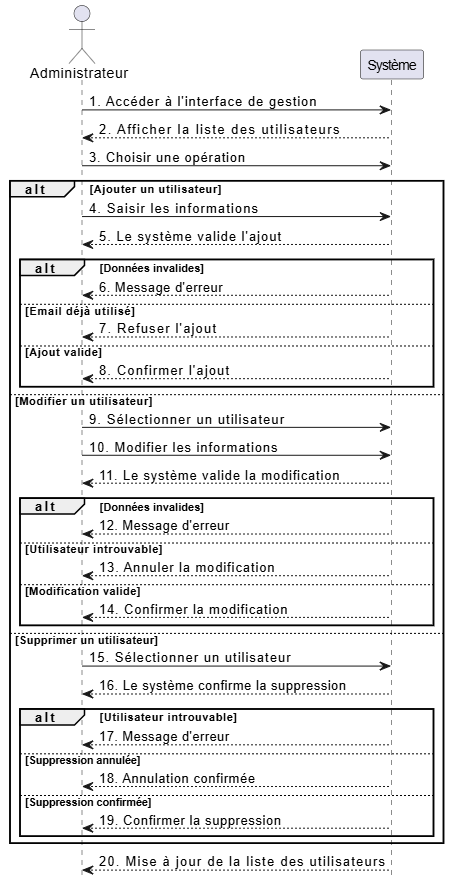
\includegraphics[width=0.85\textwidth]{seq_manage_users.jpg}
	\caption{Diagramme de séquence système du cas d’utilisation « Gérer les utilisateurs »}
	\label{fig:seq_manage_users}
\end{figure}

\FloatBarrier

\section{Conception}
\subsection{Conception statique}

\subsubsection{Diagramme de classes du Sprint 1}

Je constate que le diagramme de classes montre la structure du système pendant le premier sprint. Le diagramme de classes met en avant les classes principales : l’utilisateur, l’administrateur, le rôle et la facture.

\begin{figure}[H]
	\centering
	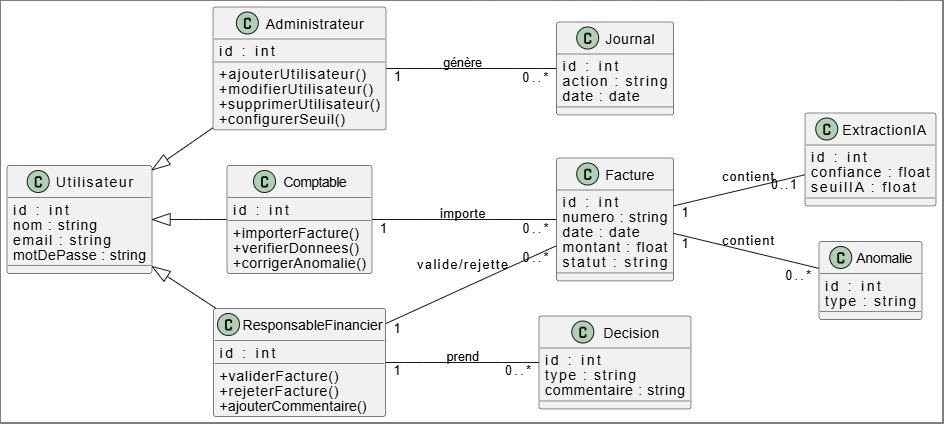
\includegraphics[width=0.85\textwidth]{diagramme_classe.jpg}
	\caption{Diagramme de classes du Sprint 1}
	\label{fig:class_sprint1}
\end{figure}

\FloatBarrier
\subsection{Conception dynamique}

\subsubsection{Diagramme de séquence détaillé du cas d’utilisation « S’authentifier »}

Le diagramme de séquence détaillé suivant illustre les interactions entre l’interface d’authentification, le contrôleur, le service utilisateur et la base de données lors du processus d’authentification.

\begin{figure}[H]
	\centering
	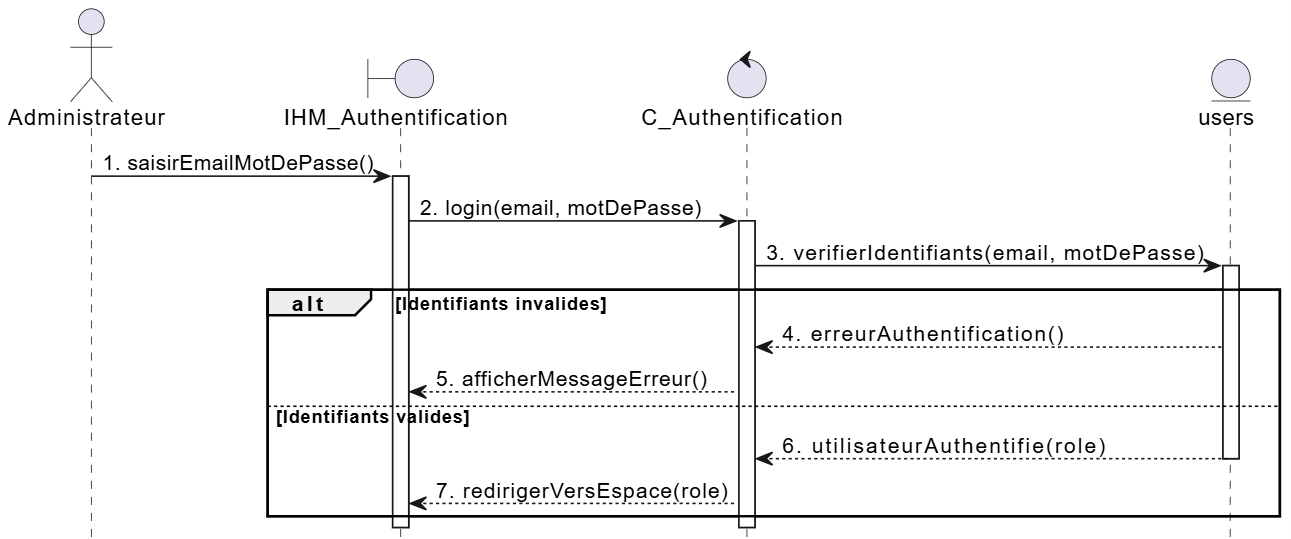
\includegraphics[width=0.85\textwidth]{seq_auth_detail.jpg}
	\caption{Diagramme de séquence détaillé du cas d’utilisation « S’authentifier »}
	\label{fig:seq_auth_detail}
\end{figure}

\FloatBarrier

\subsubsection{Diagramme de séquence détaillé du cas d’utilisation « Gérer les utilisateurs »}

Le diagramme de séquence ci-dessous montre comment l’administrateur, l’interface de gestion des utilisateurs, le contrôleur, le service utilisateur et la base de données interagissent pendant la gestion des comptes.

\begin{figure}[H]
	\centering
	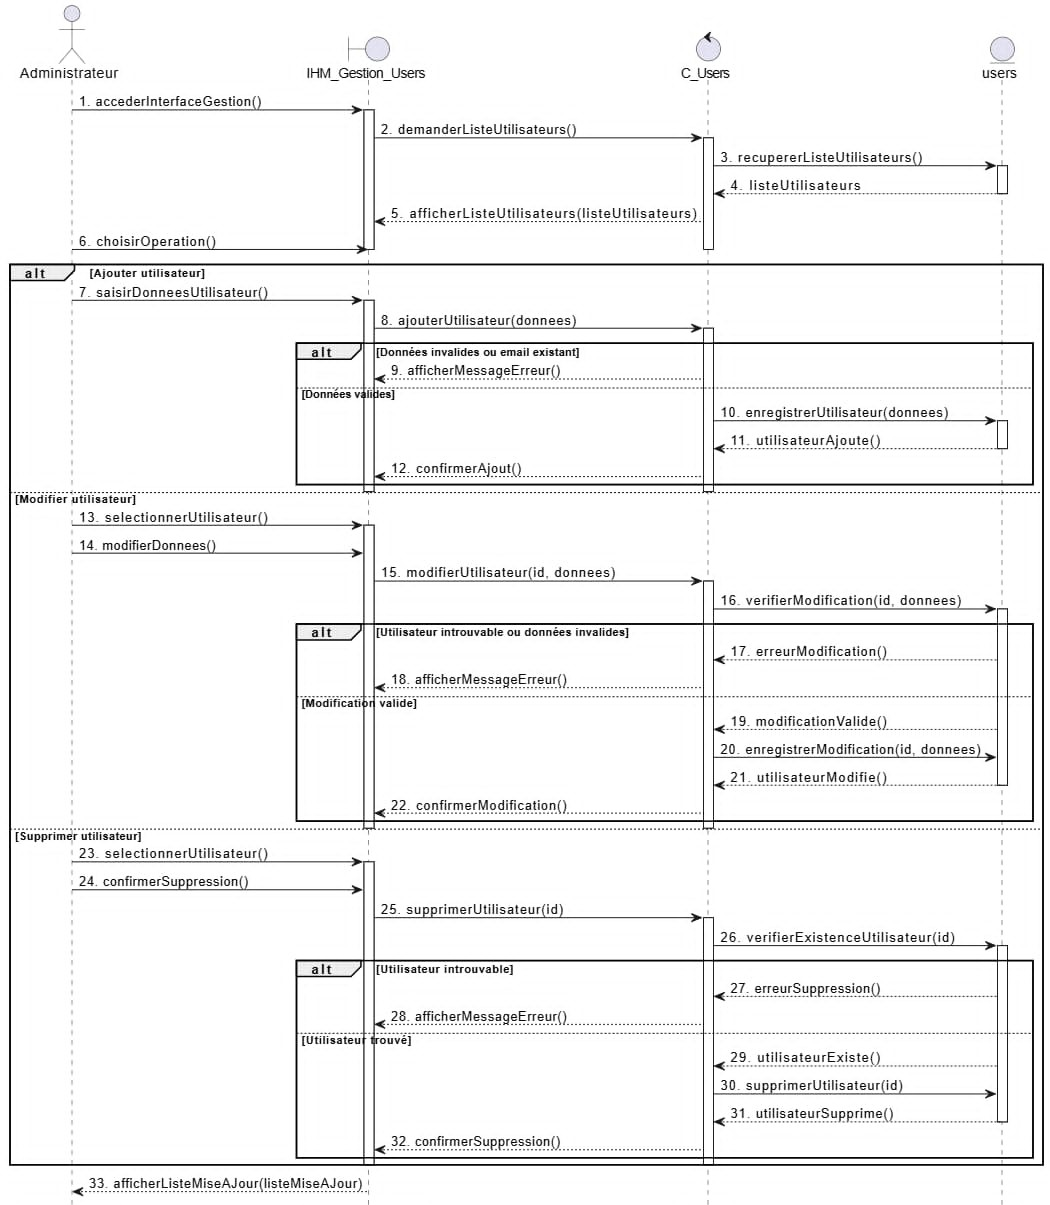
\includegraphics[width=0.85\textwidth]{seq_manage_users_detail.jpg}
	\caption{Diagramme de séquence détaillé du cas d’utilisation « Gérer les utilisateurs »}
	\label{fig:seq_manage_users_detail}
\end{figure}

\FloatBarrier


\section{Implémentation}

\subsection{Dictionnaire de données}

\subsubsection{Table utilisateur}

\renewcommand{\arraystretch}{1.3}

\begin{table}[H]
	\centering
	\footnotesize
	
	\begin{tabularx}{\textwidth}{|p{3cm}|p{2.5cm}|p{3.5cm}|X|}
		\hline
		
		\rowcolor{blue!20}
		\textbf{Nom du champ}
		&
		\textbf{Type}
		&
		\textbf{Contraintes}
		&
		\textbf{Description}
		\\ \hline
		
		id\_utilisateur
		&
		BIGINT
		&
		PRIMARY KEY
		&
		Identifiant unique de l’utilisateur.
		\\ \hline
		
		nom
		&
		VARCHAR
		&
		NOT NULL
		&
		Nom complet de l’utilisateur.
		\\ \hline
		
		email
		&
		VARCHAR
		&
		UNIQUE, NOT NULL
		&
		Adresse email utilisée pour l’authentification.
		\\ \hline
		
		motdepasse
		&
		VARCHAR
		&
		NOT NULL
		&
		Mot de passe chiffré de l’utilisateur.
		\\ \hline
		
		role
		&
		VARCHAR
		&
		NOT NULL
		&
		Rôle attribué à l’utilisateur.
		\\ \hline
		
	\end{tabularx}
	
	\caption{Dictionnaire de données de la table utilisateur}
	\label{tab:user_table}
	
\end{table}



\subsubsection{Table importation}

\begin{table}[H]
	\centering
	\footnotesize
	
	\begin{tabularx}{\textwidth}{|p{3cm}|p{2.5cm}|p{3.5cm}|X|}
		\hline
		
		\rowcolor{blue!20}
		\textbf{Nom du champ}
		&
		\textbf{Type}
		&
		\textbf{Contraintes}
		&
		\textbf{Description}
		\\ \hline
		
		id\_import
		&
		BIGINT
		&
		PRIMARY KEY
		&
		Identifiant unique de l’importation.
		\\ \hline
		
		nomFichier
		&
		VARCHAR
		&
		NOT NULL
		&
		Nom du fichier importé.
		\\ \hline
		
		dateImport
		&
		DATETIME
		&
		NOT NULL
		&
		Date d’importation du fichier.
		\\ \hline
		
		utilisateur
		&
		BIGINT
		&
		FOREIGN KEY
		&
		Utilisateur ayant effectué l’importation.
		\\ \hline
		
		statut
		&
		VARCHAR
		&
		NOT NULL
		&
		État de traitement du fichier.
		\\ \hline
		
	\end{tabularx}
	
	\caption{Dictionnaire de données de la table importation}
	\label{tab:import_table}
	
\end{table}
\section{Réalisation}

\subsection{Interfaces utilisateur}

\subsubsection{Interface de connexion}

L’interface de connexion donne à l’utilisateur un accès sécurisé au système. L’interface de connexion comprend les champs pour saisir l’adresse email et le mot de passe. Le système valide les informations saisies. Le système redirige l’utilisateur vers son espace selon le rôle de l’utilisateur.

\begin{figure}[H]
	\centering
	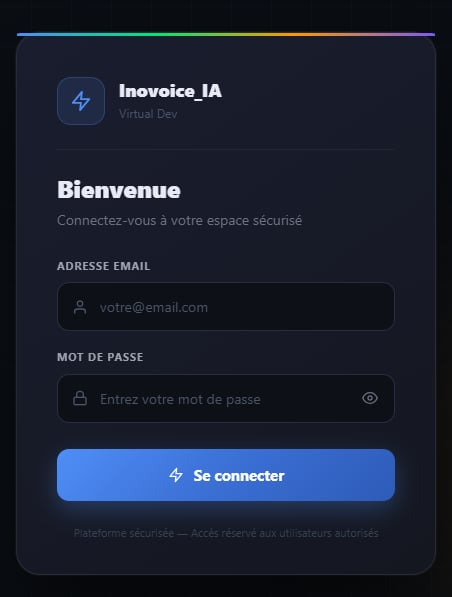
\includegraphics[width=0.4\textwidth]{login.jpg}
	\caption{Interface de connexion du système}
	\label{fig:login}
\end{figure}

\FloatBarrier

\subsubsection{Interface de liste des utilisateurs}

Cette interface permet à l’administrateur de voir la liste des utilisateurs du système. L’administrateur peut aussi ajouter, modifier ou supprimer un compte utilisateur.

\begin{figure}[H]
	\centering
	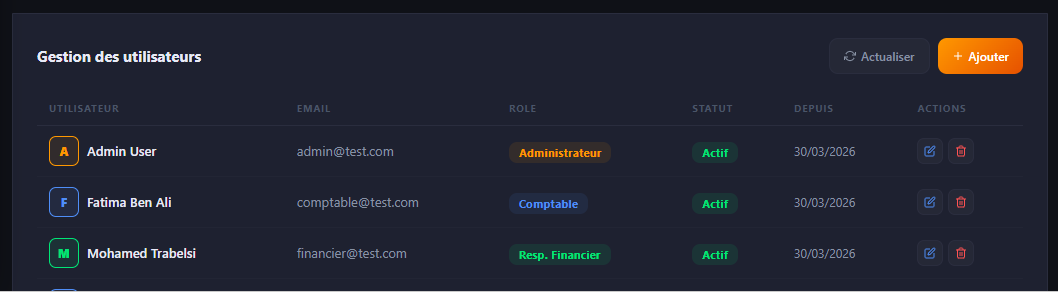
\includegraphics[width=0.65\textwidth]{users_list.jpg}
	\caption{Interface de liste des utilisateurs}
	\label{fig:users_list}
\end{figure}

\FloatBarrier

\subsubsection{Interface d’ajout d’un utilisateur}

L’administrateur utilise l’interface pour créer un nouveau compte utilisateur. L’interface comprend les champs nécessaires : le nom, l’adresse email, le mot de passe et le rôle de l’utilisateur.

\begin{figure}[H]
	\centering
	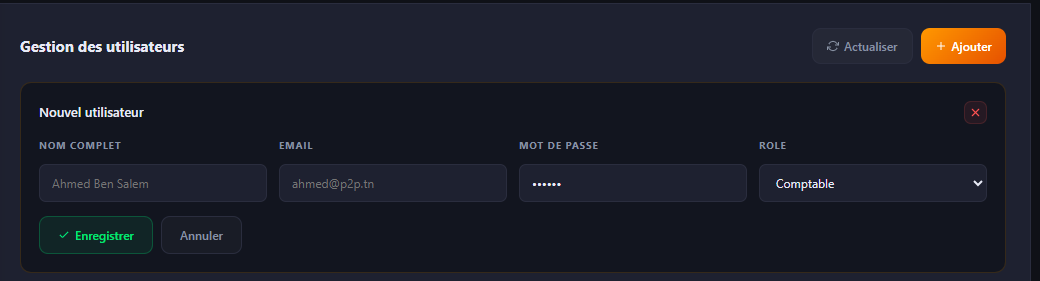
\includegraphics[width=0.65\textwidth]{add_user.jpg}
	\caption{Interface d’ajout d’un utilisateur}
	\label{fig:add_user}
\end{figure}

\FloatBarrier

\subsubsection{Interface de modification d’un utilisateur}

L’administrateur modifie les informations d’un utilisateur existant grâce à l’interface. L’interface propose des champs déjà remplis pour simplifier la mise à jour des données avant la validation.

\begin{figure}[H]
	\centering
	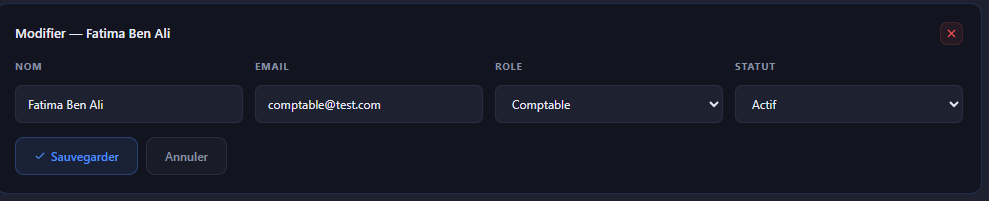
\includegraphics[width=0.75\textwidth]{edit_user.jpg}
	\caption{Interface de modification d’un utilisateur}
	\label{fig:edit_user}
\end{figure}

\FloatBarrier

\subsubsection{Interface d’importation des factures}

L’interface permet au comptable d’importer une facture dans le système. Après la sélection du fichier, le traitement démarre pour préparer l’extraction automatique des données.

\begin{figure}[H]
	\centering
	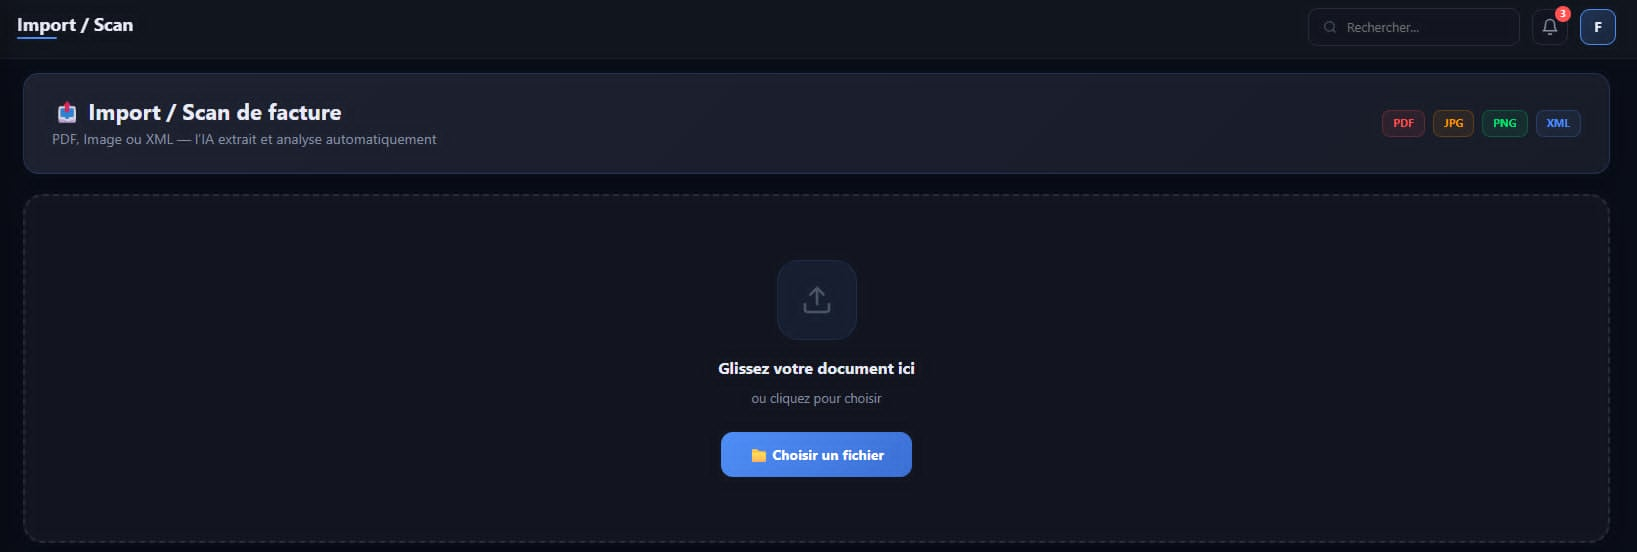
\includegraphics[width=0.75\textwidth]{ui_import.jpg}
	\caption{Interface d’importation des factures}
	\label{fig:ui_import}
\end{figure}

\FloatBarrier

\subsubsection{Interface d’affichage des résultats OCR}

Cette interface permet au comptable de consulter les données extraites automatiquement à partir de la facture importée. L’interface montre les informations principales : le fournisseur, la date, les montants et le numéro de facture.

\begin{figure}[H]
	\centering
	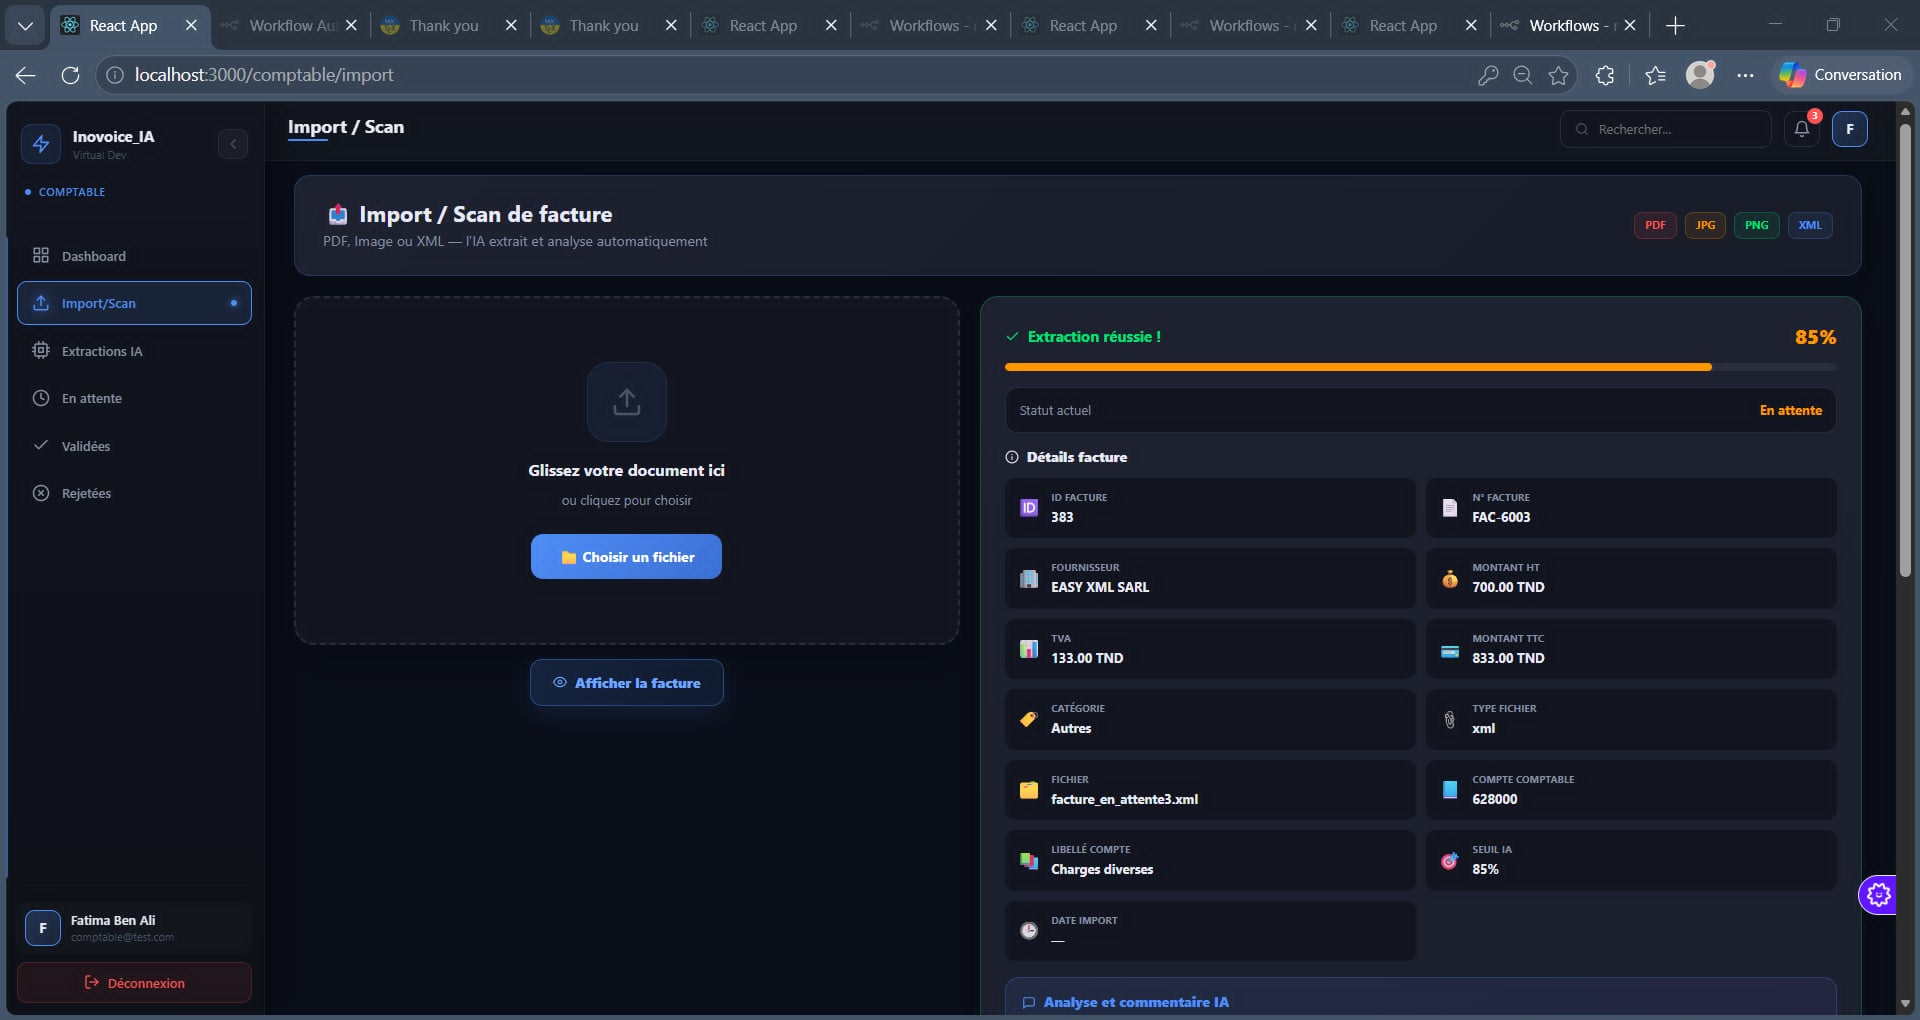
\includegraphics[width=0.75\textwidth]{ui_ocr_result.jpg}
	\caption{Interface d’affichage des résultats OCR}
	\label{fig:ui_ocr_result}
\end{figure}
\section{Tests Postman}

Cette section présente les tests réalisés avec l’outil Postman afin de vérifier le bon fonctionnement des API développées durant le Sprint 1.  
Ces tests concernent principalement l’authentification des utilisateurs, la gestion des comptes ainsi que les opérations de base liées aux utilisateurs.

L’objectif de ces tests est de s’assurer que chaque requête envoyée au backend retourne une réponse correcte et que les données sont bien traitées par le système.

\renewcommand{\arraystretch}{1.5}

\begin{longtable}{|>{\centering\arraybackslash}m{6cm}|>{\centering\arraybackslash}m{10cm}|}
	\hline
	
	\rowcolor{blue!20}
	\textbf{Description} & \textbf{Capture}
	\\ \hline
	
	Cette requête permet à l’utilisateur de se connecter à la plateforme en utilisant son adresse email et son mot de passe. 
	Elle permet de vérifier l’API d’authentification ainsi que la redirection de l’utilisateur selon son rôle.
	&
	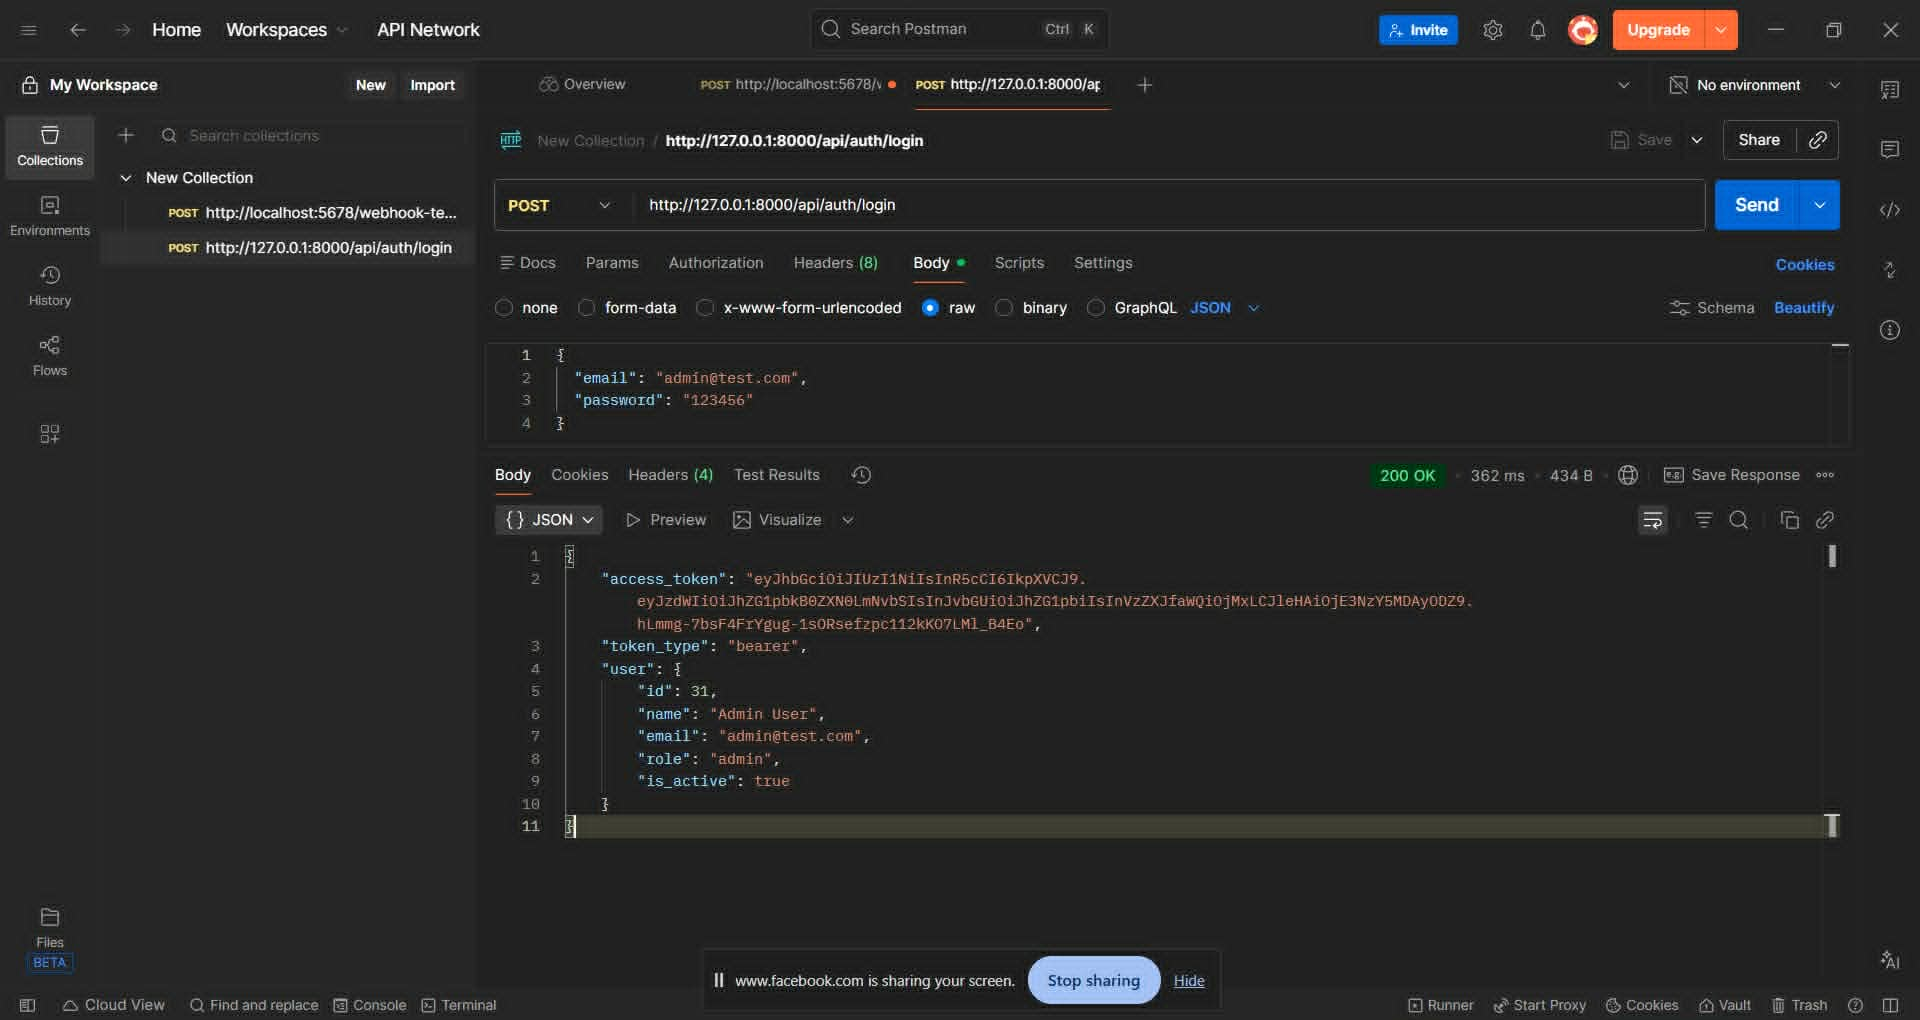
\includegraphics[width=8cm]{figures/postman_login.jpg}
	\\ \hline
	
	Cette requête permet à l’administrateur d’ajouter un nouvel utilisateur dans le système. 
	Elle vérifie l’enregistrement des informations saisies telles que le nom, l’email, le mot de passe et le rôle.
	&
	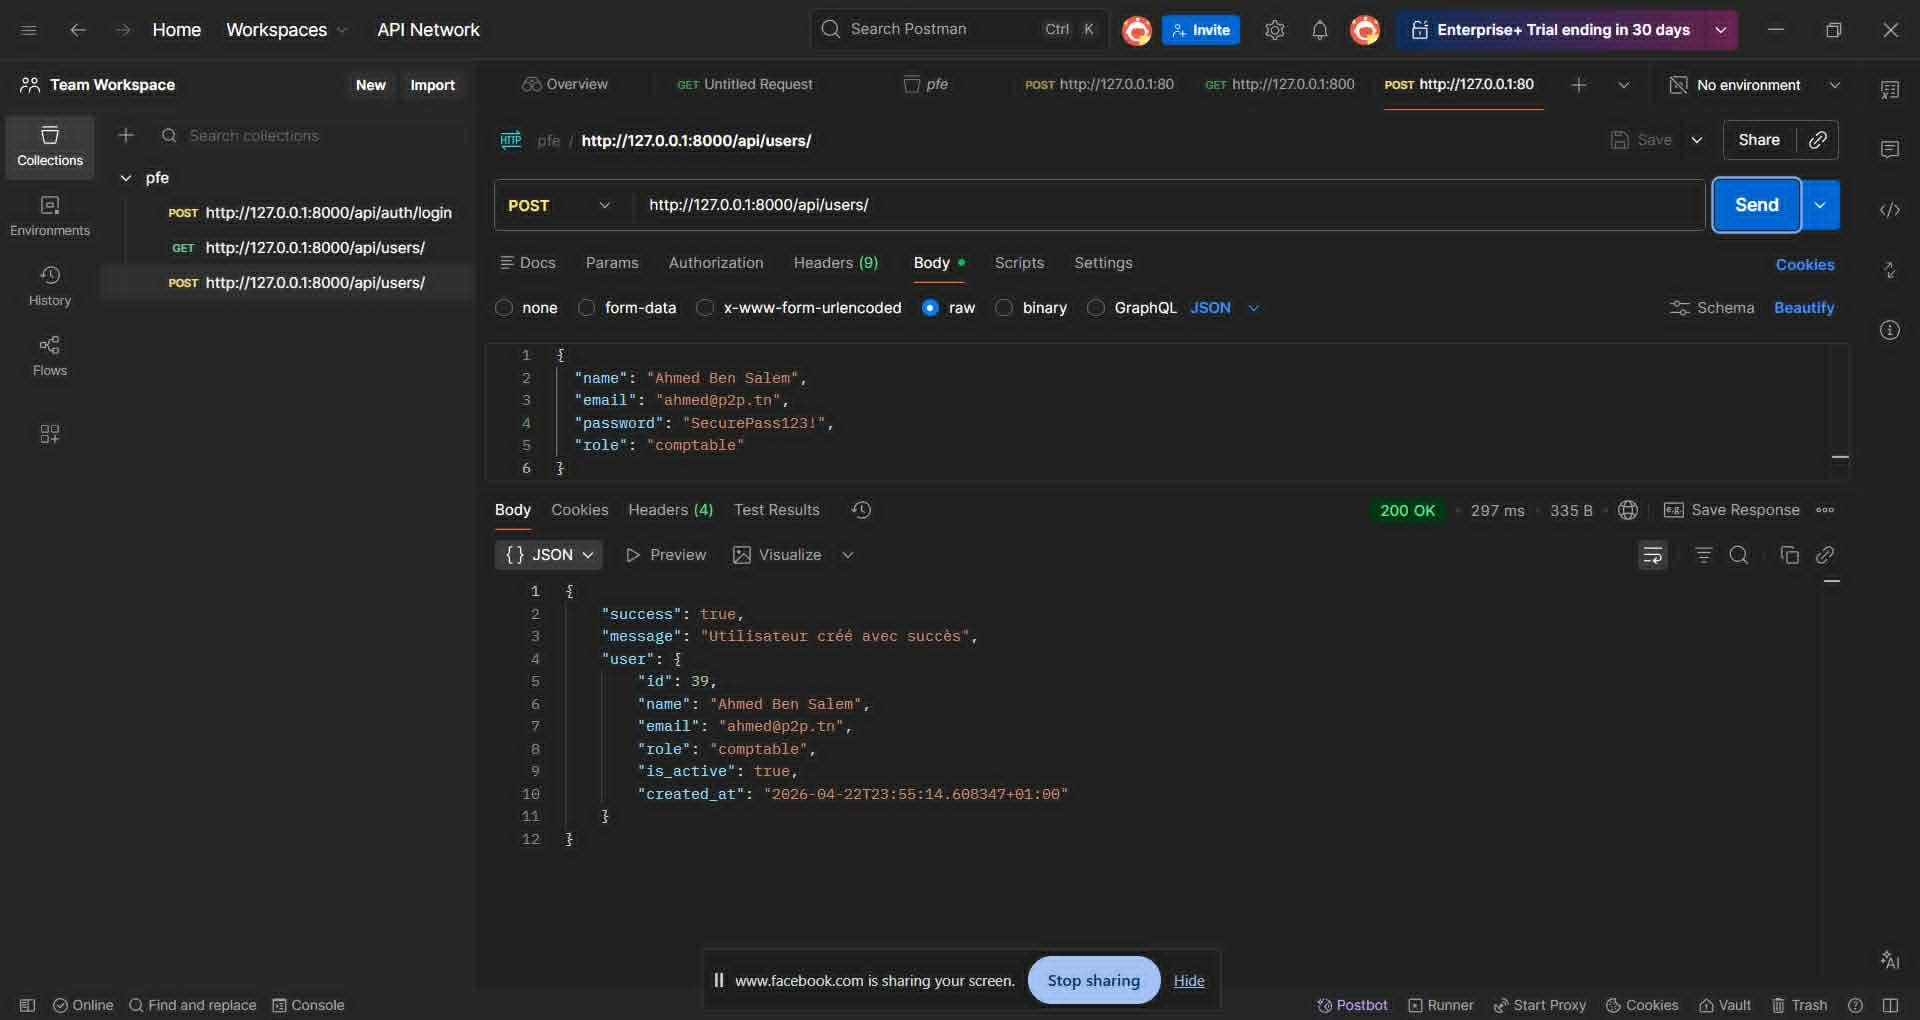
\includegraphics[width=8cm]{figures/postman_add_user.jpg}
	\\ \hline
	
	Cette requête permet de modifier les informations d’un utilisateur existant. 
	Elle permet de tester la mise à jour des données dans la base et de vérifier que les changements sont bien sauvegardés.
	&
	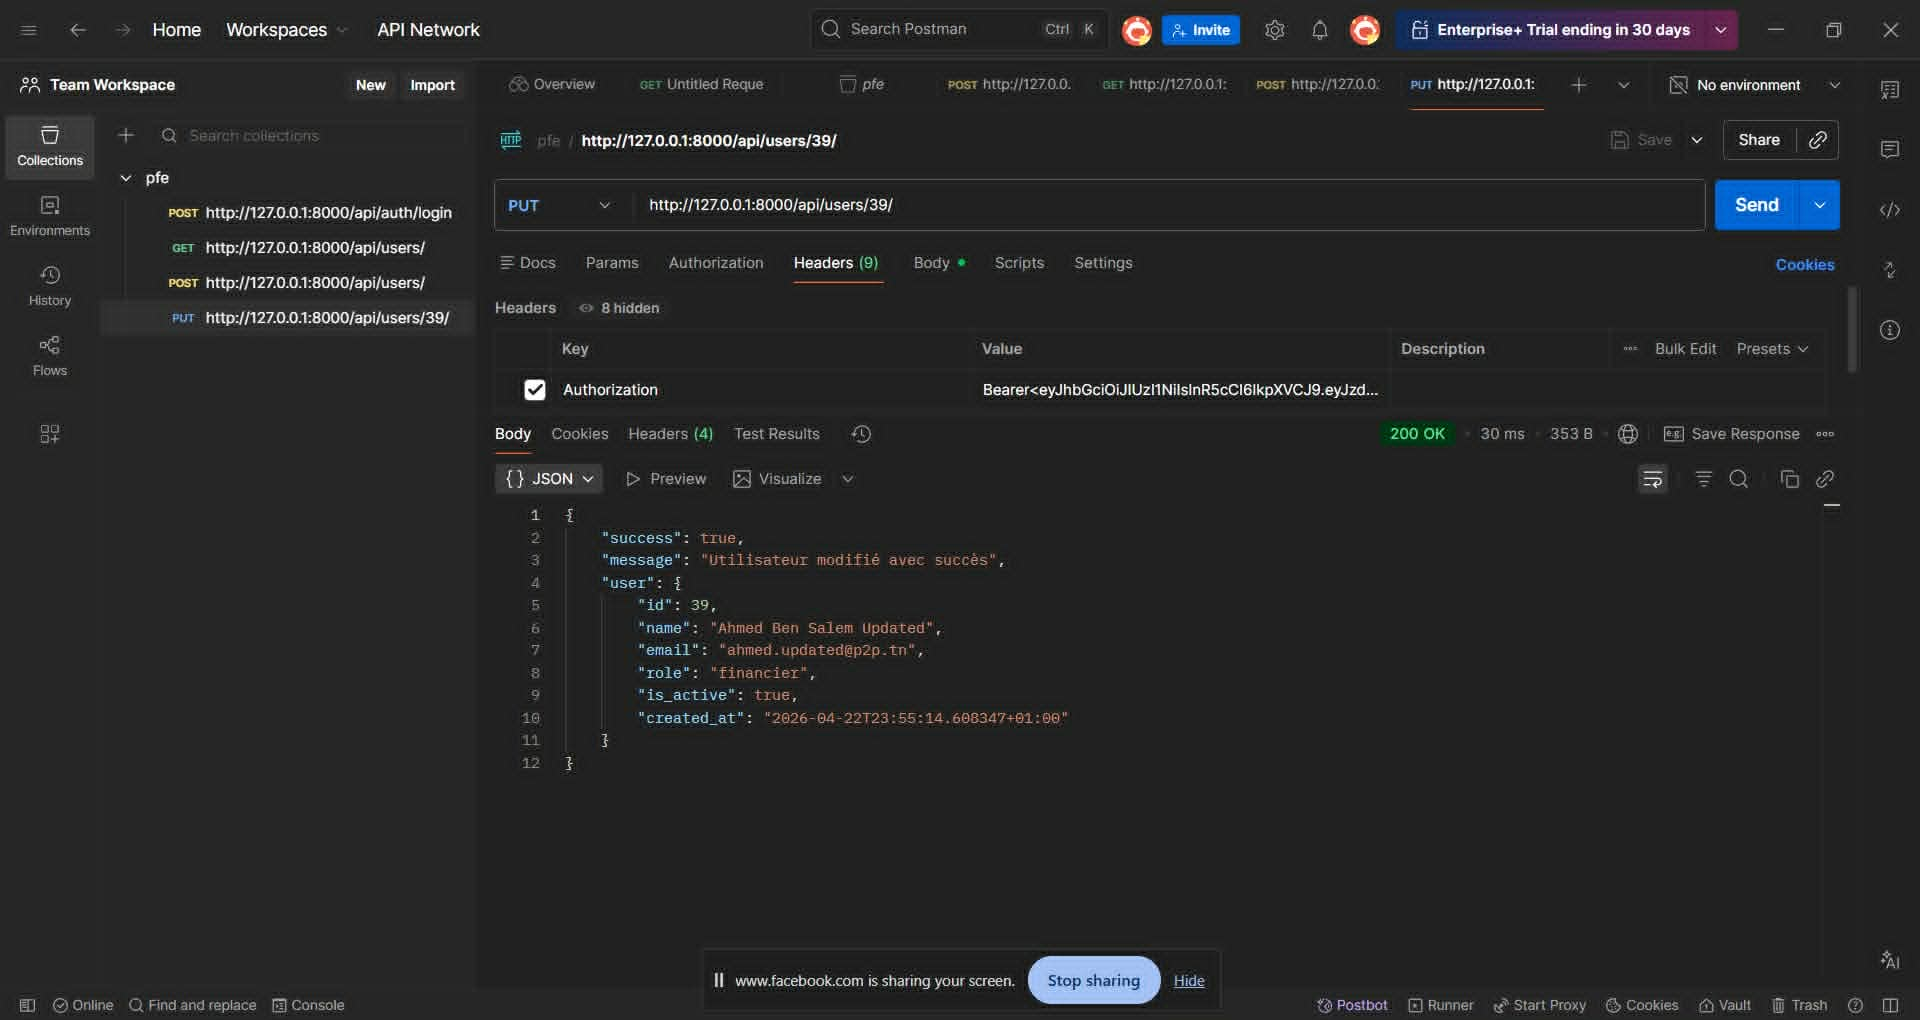
\includegraphics[width=8cm]{figures/postman_update_user.jpg}
	\\ \hline
	
	Cette requête permet de supprimer un utilisateur du système. 
	Elle vérifie que l’utilisateur sélectionné est bien supprimé de la base de données.
	&
	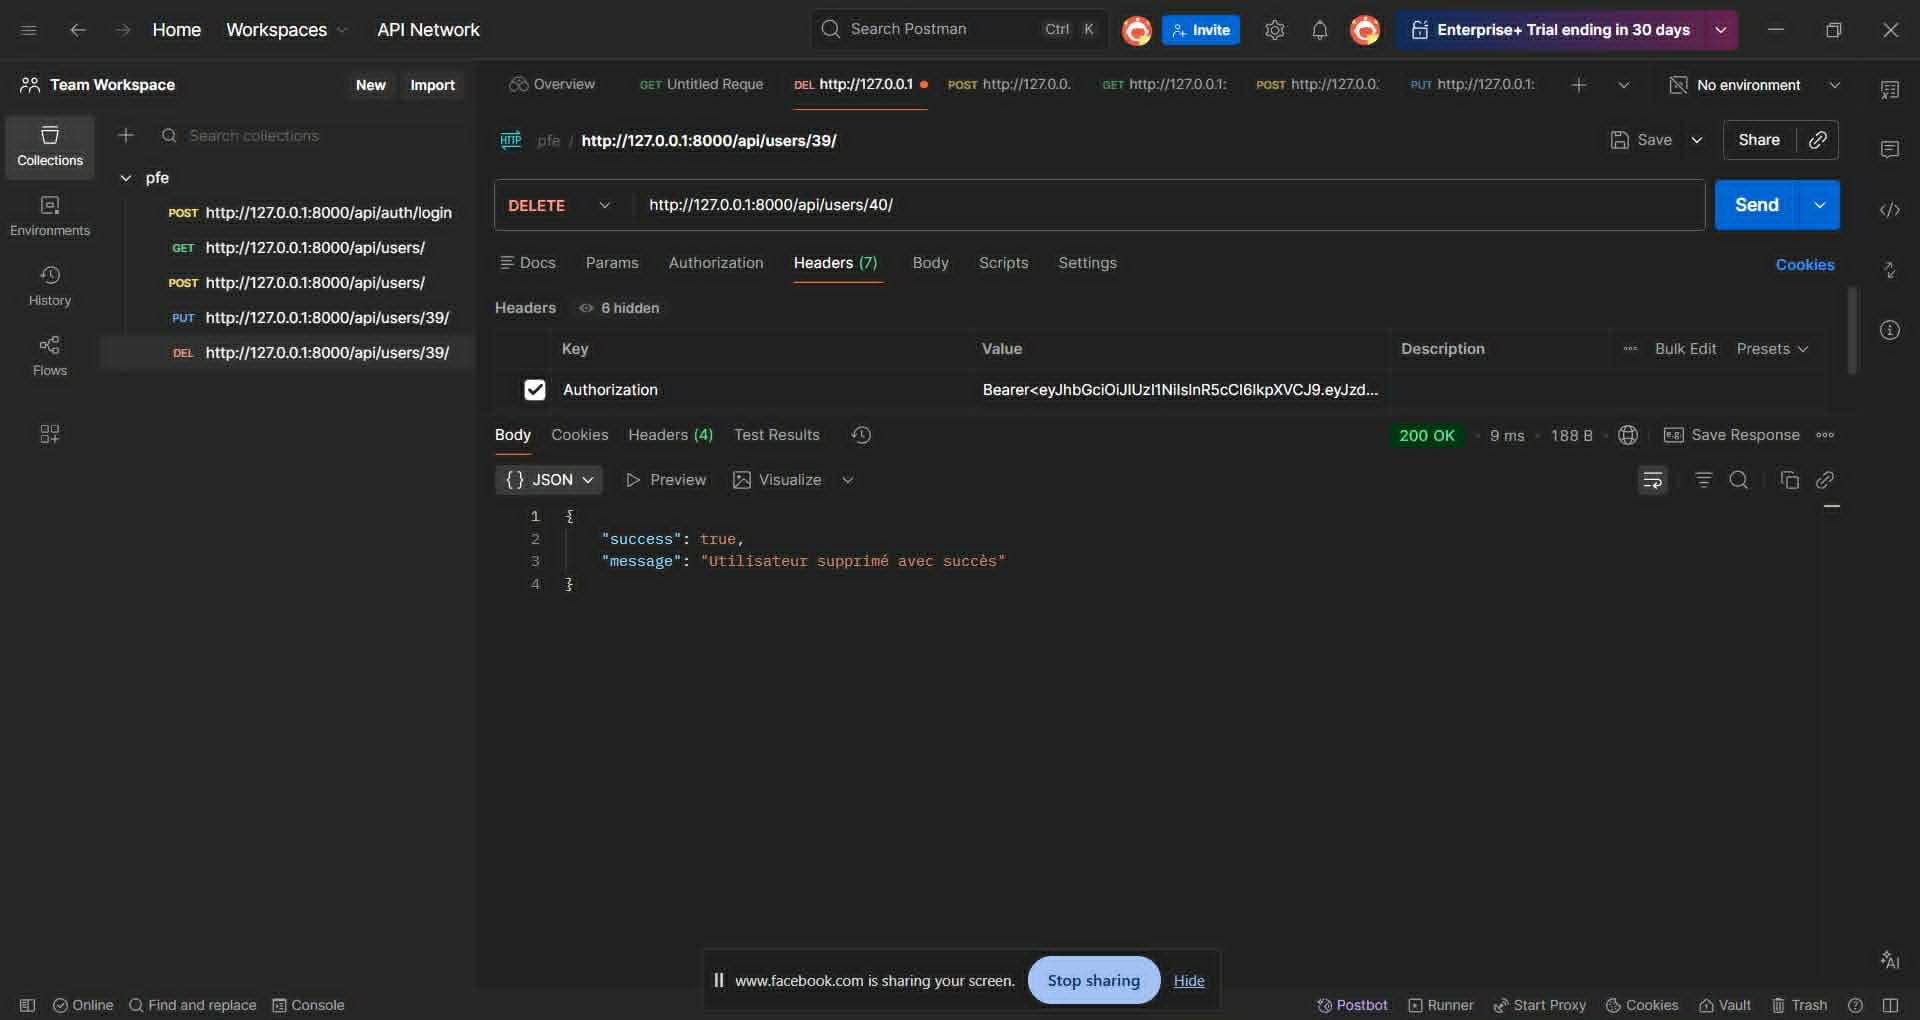
\includegraphics[width=8cm]{figures/postman_delete_user.jpg}
	\\ \hline
	
	Cette requête permet de récupérer la liste des utilisateurs enregistrés dans le système. 
	Elle sert à vérifier l’affichage des comptes existants et le bon fonctionnement de l’API de consultation.
	&
	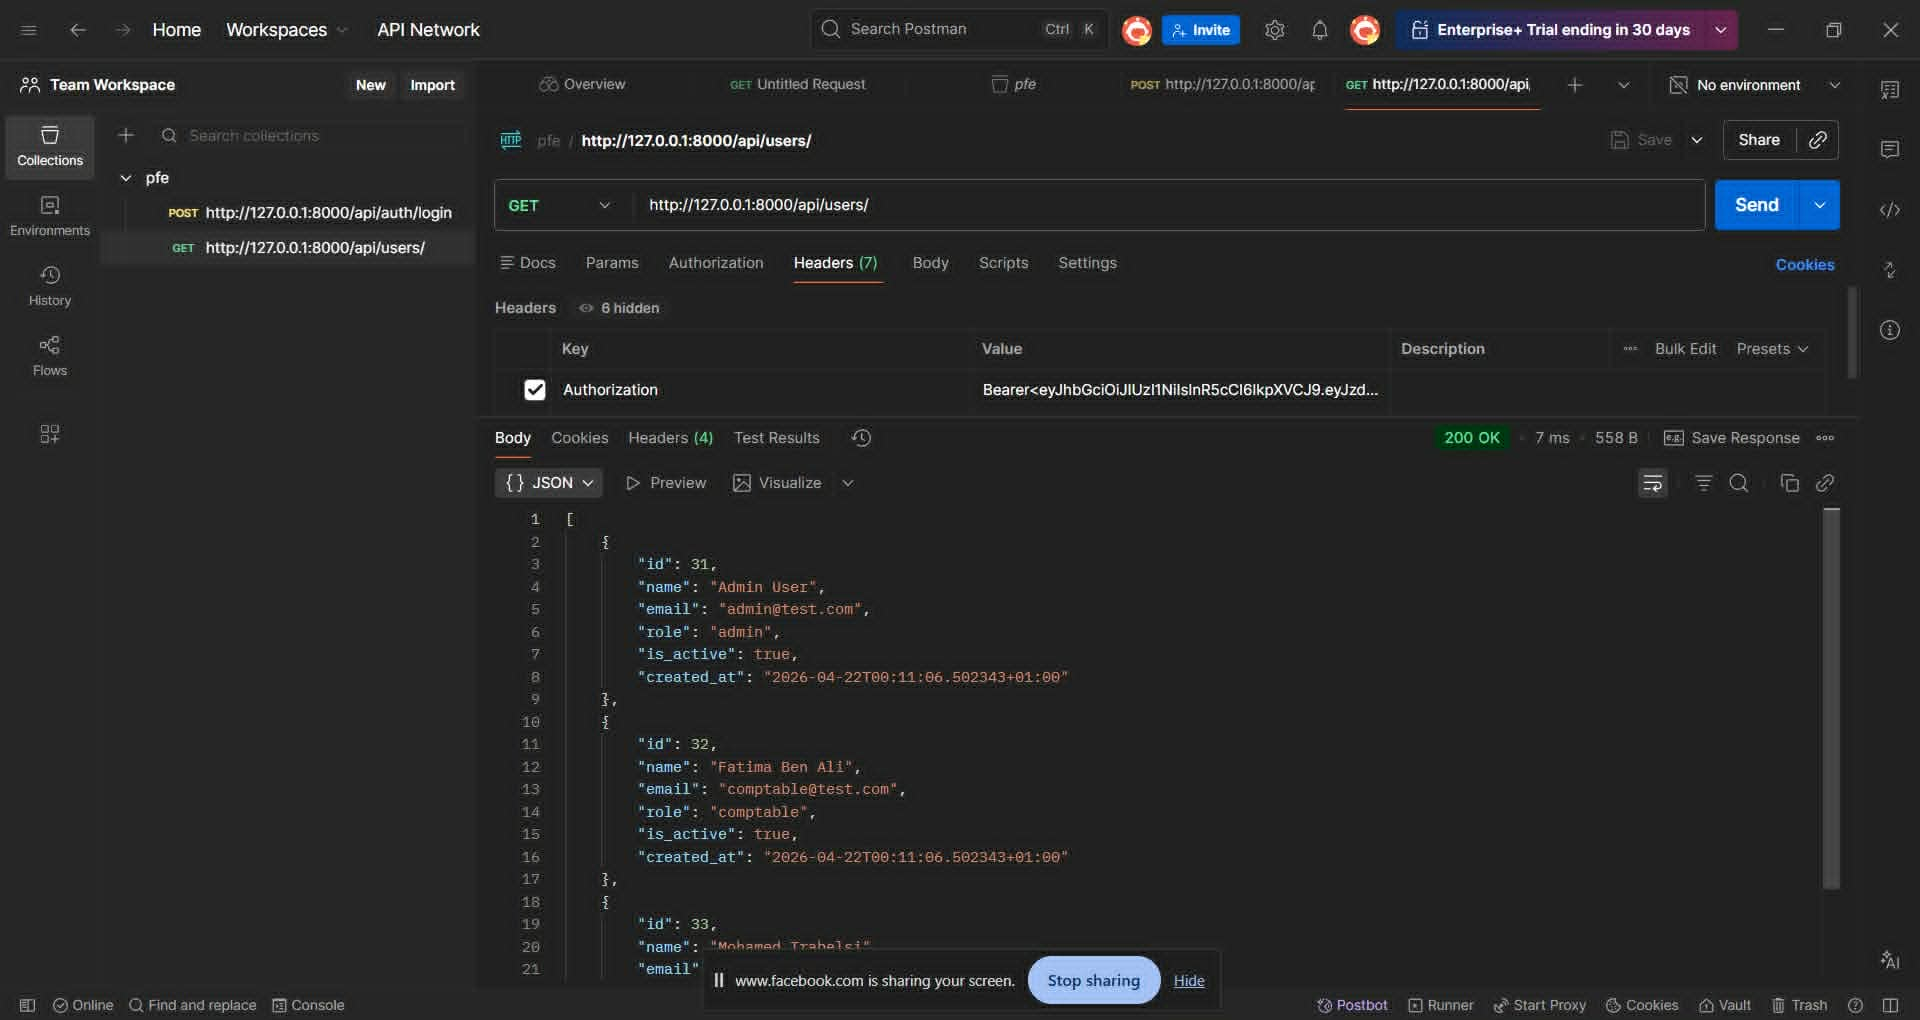
\includegraphics[width=8cm]{figures/postman_users.jpg}
	\\ \hline
	
	\caption{Tests Postman du Sprint 1}
\end{longtable}
\vspace{-0.2cm}
\subsection{Revue de Sprint}

La revue du Sprint 1 a permis de présenter les fonctionnalités réalisées liées à
l’authentification, à la gestion des utilisateurs ainsi qu’à l’importation et à
l’extraction des factures via OCR et intelligence artificielle. Cette étape a permis
de vérifier le bon fonctionnement des interfaces développées, des API
d’authentification ainsi que des mécanismes d’importation et de traitement des données.

\vspace{-0.2cm}
\noindent\textbf{Burndown Chart :} Le Burndown Chart du Sprint 1 permet de visualiser
l’évolution du travail restant durant les fonctionnalités d’authentification, de gestion
des utilisateurs et d’extraction des données. Le graphique montre une progression
régulière des tâches jusqu’à la finalisation du sprint. Comme présenté dans la figure
\ref{fig:brun1}.

\vspace{-0.4cm}
\begin{figure}[H]
	\centering
	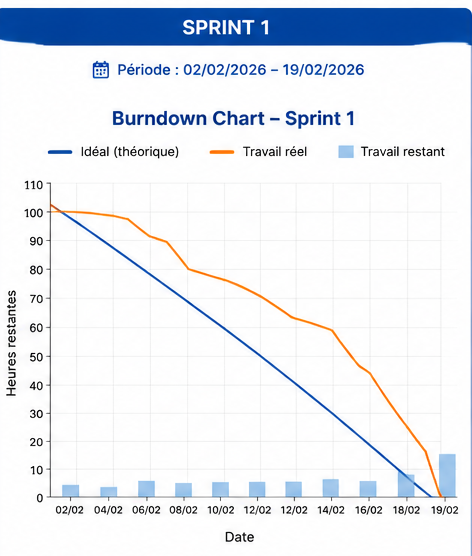
\includegraphics[width=0.5\textwidth]{burndown_sprint1.jpg}
	\caption{Diagramme de Burndown Chart du Sprint 1}
	\label{fig:brun1}
\end{figure}
\begin{table}[H]
	\centering
	\renewcommand{\arraystretch}{1.3}
	
	\begin{tabular}{|c|p{5cm}|c|}
		\hline
		\rowcolor{blue!20}
		\textbf{ID User Story} & \textbf{Fonctionnalité} & \textbf{Estimation} \\
		\hline
		
		1.1 & Authentification des utilisateurs & 3 \\
		\hline
		
		1.2 & Gestion des utilisateurs & 3 \\
		\hline
		
		1.3 & Importation des factures & 4 \\
		\hline
		
		1.4 & Extraction OCR des données & 5 \\
		\hline
		
		1.5 & Tests Postman des API & 2 \\
		\hline
		
		1.6 & Intégration Frontend / Backend & 3 \\
		\hline
		
		\multicolumn{2}{|c|}{\textbf{Vélocité totale estimée}} & \textbf{20} \\
		\hline
		
	\end{tabular}
	
	\caption{Calcul de vélocité estimée du Sprint 1}
\end{table}
\section{Conclusion}

Dans ce chapitre, nous avons présenté les fonctionnalités développées durant le Sprint 1. Nous avons réalisé l’authentification, la gestion des utilisateurs ainsi que l’importation et l’extraction automatique des données des factures.
\chapter{Sprint 2 : Traitement et consultation des données}
\newpage
\section{Introduction}

Le quatrième chapitre présente les fonctionnalités développées dans le Sprint 2. Nous y décrivons la gestion des factures, la consultation des résultats d’extraction, les tableaux de bord ainsi que la configuration des seuils de l’intelligence artificielle.

\section{Backlog du Sprint}

\renewcommand{\arraystretch}{1.25}

\begin{table}[H]
	\centering
	\footnotesize
	
	\begin{tabularx}{\textwidth}{|c|p{3.6cm}|c|X|c|}
		\hline
		
		\rowcolor{blue!20}
		\textbf{ID} &
		\textbf{User Story} &
		\textbf{ID-US} &
		\textbf{Tâche} &
		\textbf{Estimation}
		\\ \hline
		
		%====================================================
		
		\multirow{4}{*}{2.1}
		& \multirow{4}{3.6cm}{
			En tant que comptable, je veux consulter les résultats d’extraction afin de vérifier les données extraites.
		}
		& 2.1.1 & Conception UML de consultation des extractions. & \multirow{4}{*}{2 jours}
		\\ \cline{3-4}
		
		& & 2.1.2 & Développement de l’interface de consultation.
		& \\ \cline{3-4}
		
		& & 2.1.3 & Implémentation backend d’affichage des résultats.
		& \\ \cline{3-4}
		
		& & 2.1.4 & Tests et validation.
		& \\ \hline
		
		%====================================================
		
		\multirow{4}{*}{2.2}
		& \multirow{4}{3.6cm}{
			En tant que comptable, je veux gérer les factures selon leurs statuts afin de suivre leur traitement.
		}
		& 2.2.1 & Conception UML de gestion des factures. & \multirow{4}{*}{2 jours}
		\\ \cline{3-4}
		
		& & 2.2.2 & Développement de l’interface des statuts.
		& \\ \cline{3-4}
		
		& & 2.2.3 & Implémentation backend de gestion des statuts.
		& \\ \cline{3-4}
		
		& & 2.2.4 & Tests et validation.
		& \\ \hline
		
		%====================================================
		
		\multirow{4}{*}{2.3}
		& \multirow{4}{3.6cm}{
			En tant que comptable, je veux consulter le tableau de bord afin de visualiser les indicateurs et statistiques.
		}
		& 2.3.1 & Conception du tableau de bord. & \multirow{4}{*}{2 jours}
		\\ \cline{3-4}
		
		& & 2.3.2 & Développement des graphiques et indicateurs.
		& \\ \cline{3-4}
		
		& & 2.3.3 & Intégration des statistiques dynamiques.
		& \\ \cline{3-4}
		
		& & 2.3.4 & Tests et validation.
		& \\ \hline
		
		%====================================================
		
		\multirow{4}{*}{2.4}
		& \multirow{4}{3.6cm}{
			En tant qu’administrateur, je veux définir les seuils de confiance de l’IA afin d’adapter le traitement automatique.
		}
		& 2.4.1 & Conception UML de configuration IA. & \multirow{4}{*}{1 jour}
		\\ \cline{3-4}
		
		& & 2.4.2 & Développement de l’interface de configuration.
		& \\ \cline{3-4}
		
		& & 2.4.3 & Implémentation backend des seuils IA.
		& \\ \cline{3-4}
		
		& & 2.4.4 & Tests et validation.
		& \\ \hline
		
	\end{tabularx}
	
	\caption{Backlog détaillé du Sprint 2}
	\label{tab:backlog_sprint2}
	
\end{table}

\FloatBarrier


%====================================================
\section{Analyse}

\subsection{Analyse fonctionnelle}

\subsubsection{Diagramme de cas d’utilisation}

Le diagramme de cas d’utilisation montre les fonctions principales du deuxième sprint. Le comptable consulte les résultats de l’extraction, le comptable gère les factures et le comptable utilise le tableau de bord. L’administrateur configure les seuils de confiance de l’IA.

\begin{figure}[H]
	\centering
	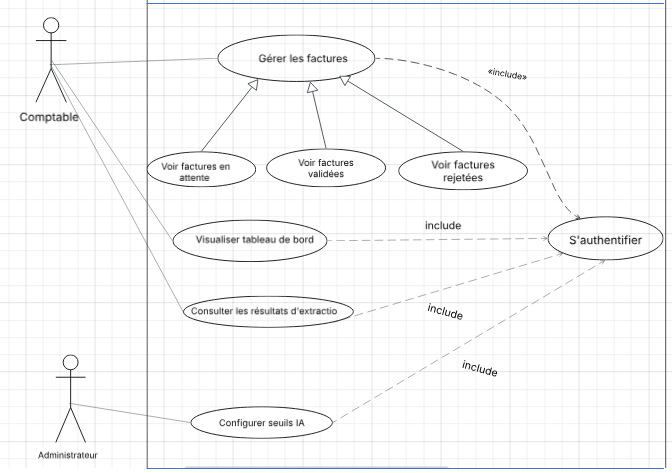
\includegraphics[width=0.9\textwidth]{usecase_sprint2.jpg}
	\caption{Diagramme de cas d’utilisation du Sprint 2}
	\label{fig:usecase_sprint2}
\end{figure}

\FloatBarrier

%====================================================
\subsubsection{Description textuelle des cas d’utilisation}

\subsubsection*{Cas d’utilisation : Consulter les extractions}

\begin{table}[H]
	\centering
	\renewcommand{\arraystretch}{1.35}
	\rowcolors{2}{gray!10}{white}
	
	\begin{tabularx}{\textwidth}{|p{3.8cm}|X|}
		\hline
		\rowcolor{blue!20}
		\textbf{Use Case} & \textbf{Consulter les extractions} \\ \hline
		
		\textbf{Acteur} & Comptable \\ \hline
		
		\textbf{Description} & Le comptable peut consulter les résultats d’extraction automatique des factures. Les résultats affichent les données extraites, le statut et le score de confiance de l’IA. \\ \hline
		
		\textbf{Pré-condition} & Le comptable est authentifié et des factures ont été traitées par le système. \\ \hline
		
		\rowcolor{blue!10}
		\textbf{Scénario nominal} &
		1- Le comptable ouvre l’interface des extractions. \newline
		2- Le système récupère les résultats d’extraction disponibles. \newline
		3- Le système affiche la liste des extractions. \newline
		4- Le comptable consulte les informations affichées. \newline
		5- Le comptable peut consulter les détails d’une extraction. \\ \hline
		
		\textbf{Post-condition} & Les résultats d’extraction sont affichés. \\ \hline
		
		\rowcolor{blue!10}
		\textbf{Scénarios alternatifs} &
		1- Aucune extraction disponible. \newline
		1.1- Le système affiche un message informatif. \newline
		2- Erreur lors du chargement des résultats. \newline
		2.1- Le système affiche un message d’erreur. \\ \hline
		
	\end{tabularx}
	
	\caption{Description textuelle du cas d’utilisation « Consulter les extractions »}
	\label{tab:consulter_extractions}
\end{table}

\FloatBarrier

%====================================================
\subsubsection*{Cas d’utilisation : Gérer les factures}

\begin{table}[H]
	\centering
	\renewcommand{\arraystretch}{1.5}
	\small
	
	\begin{tabularx}{\textwidth}{|p{4.5cm}|X|}
		\hline
		\rowcolor{blue!20}
		
		\textbf{Nom du cas d’utilisation}
		& Gérer les factures \\ \hline
		
		\textbf{Description brève}
		& Le comptable consulte les factures du système selon leurs statuts : en attente, validées ou anomalies. \\ \hline
		
		\textbf{Acteurs primaires}
		& Comptable \\ \hline
		
		\textbf{Acteurs secondaires}
		& Aucun \\ \hline
		
		\textbf{Pré-condition}
		& Le comptable doit être authentifié. \\ \hline
		
		\textbf{Scénario nominal}
		&
		1- Le comptable ouvre l’interface de gestion des factures. \newline
		
		2- Le système affiche la liste des factures. \newline
		
		3- Le comptable sélectionne la catégorie des factures à consulter. \newline
		
		4- Si le comptable sélectionne l’option « Factures en attente » : \newline
		\hspace*{0.5cm}4.1- Le système affiche les factures en attente. \newline
		\hspace*{0.5cm}4.2- Le comptable consulte les informations affichées. \newline
		
		5- Si le comptable choisit « Factures validées » : \newline
		\hspace*{0.5cm}5.1- Le système affiche les factures validées. \newline
		\hspace*{0.5cm}5.2- Le comptable consulte les informations affichées. \newline
		
		6- Si le comptable choisit « Factures anomalies » : \newline
		\hspace*{0.5cm}6.1- Le système affiche les factures avec anomalies. \newline
		\hspace*{0.5cm}6.2- Le comptable consulte les informations affichées. \newline
		
		7- Le système actualise l’affichage des factures selon la catégorie choisie. \\ \hline
		
		\textbf{Post-condition}
		& Les factures correspondant à la catégorie choisie sont affichées. \\ \hline
		
		\textbf{Scénarios alternatifs}
		&
		1- Aucune facture disponible dans la catégorie sélectionnée. \newline
		1.1- Le système affiche un message informatif. \newline
		
		2- Erreur lors du chargement des factures. \newline
		2.1- Le système affiche un message d’erreur. \\ \hline
		
	\end{tabularx}
	
	\caption{Description textuelle du cas d’utilisation « Gérer les factures »}
	\label{tab:gerer_factures}
	
\end{table}

\clearpage

\subsection{Analyse dynamique}

\subsubsection{Diagramme de séquence système du cas d’utilisation « Consulter les extractions »}

\begin{figure}[H]
	\centering
	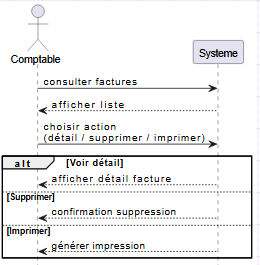
\includegraphics[width=0.6\textwidth]{seq_resultats_extraction.jpg}
	\caption{Diagramme de séquence système du cas d’utilisation « Consulter les extractions »}
	\label{fig:seq_resultats_extraction}
\end{figure}

\subsubsection{Diagramme de séquence système du cas d’utilisation « Gérer les factures »}

\begin{figure}[H]
	\centering
	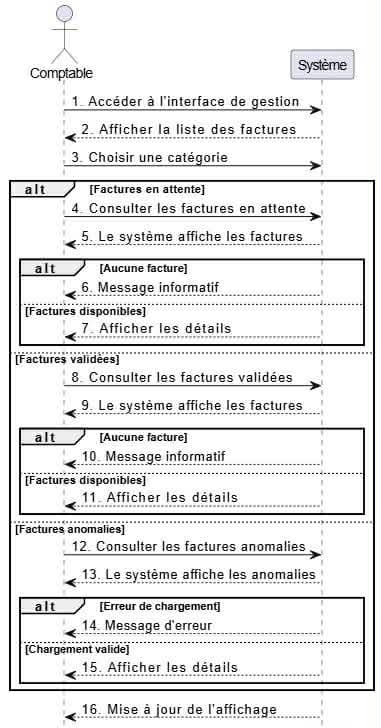
\includegraphics[width=0.6\textwidth]{seq_factures_statut.jpg}
	\caption{Diagramme de séquence système du cas d’utilisation « Gérer les factures »}
	\label{fig:seq_factures_statut}
\end{figure}

\section{Conception}
%====================================================
\subsection{Conception statique}

\subsubsection{Diagramme de classes du Sprint 2}

\begin{figure}[H]
	\centering
	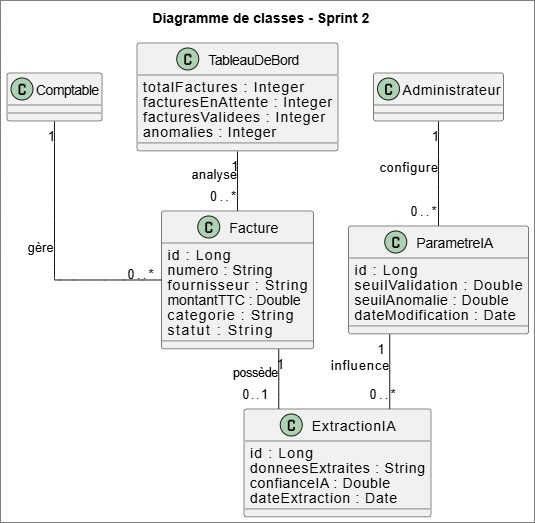
\includegraphics[width=0.85\textwidth]{class_sprint2.jpg}
	\caption{Diagramme de classes du Sprint 2}
	\label{fig:class_sprint2}
\end{figure}

\subsection{Conception dynamique}

\subsubsection{Diagramme de séquence détaillé du cas d’utilisation « Consulter les extractions »}

\begin{figure}[H]
	\centering
	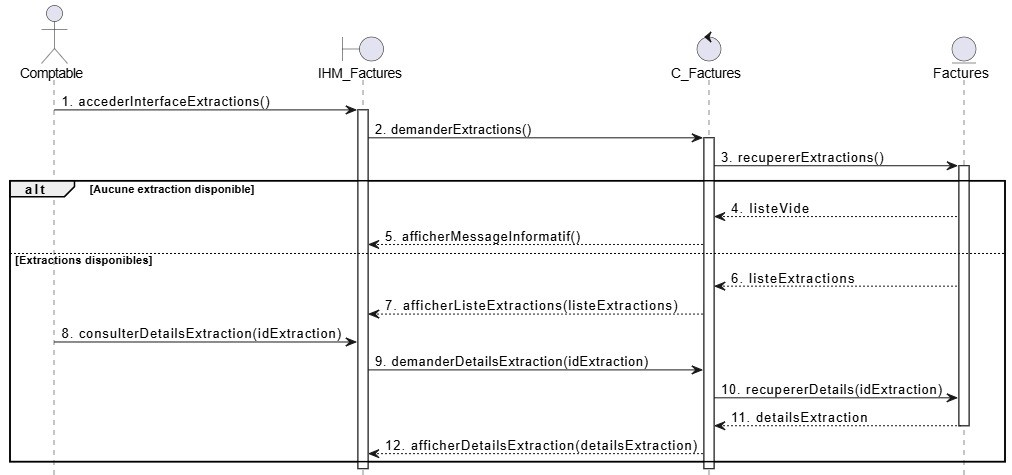
\includegraphics[width=0.65\textwidth]{seq_resultats_extraction_detail.jpg}
	\caption{Diagramme de séquence détaillé du cas d’utilisation « Consulter les extractions »}
	\label{fig:seq_resultats_extraction_detail}
\end{figure}


\subsubsection{Diagramme de séquence détaillé du cas d’utilisation « Gérer les factures »}

\begin{figure}[H]
	\centering
	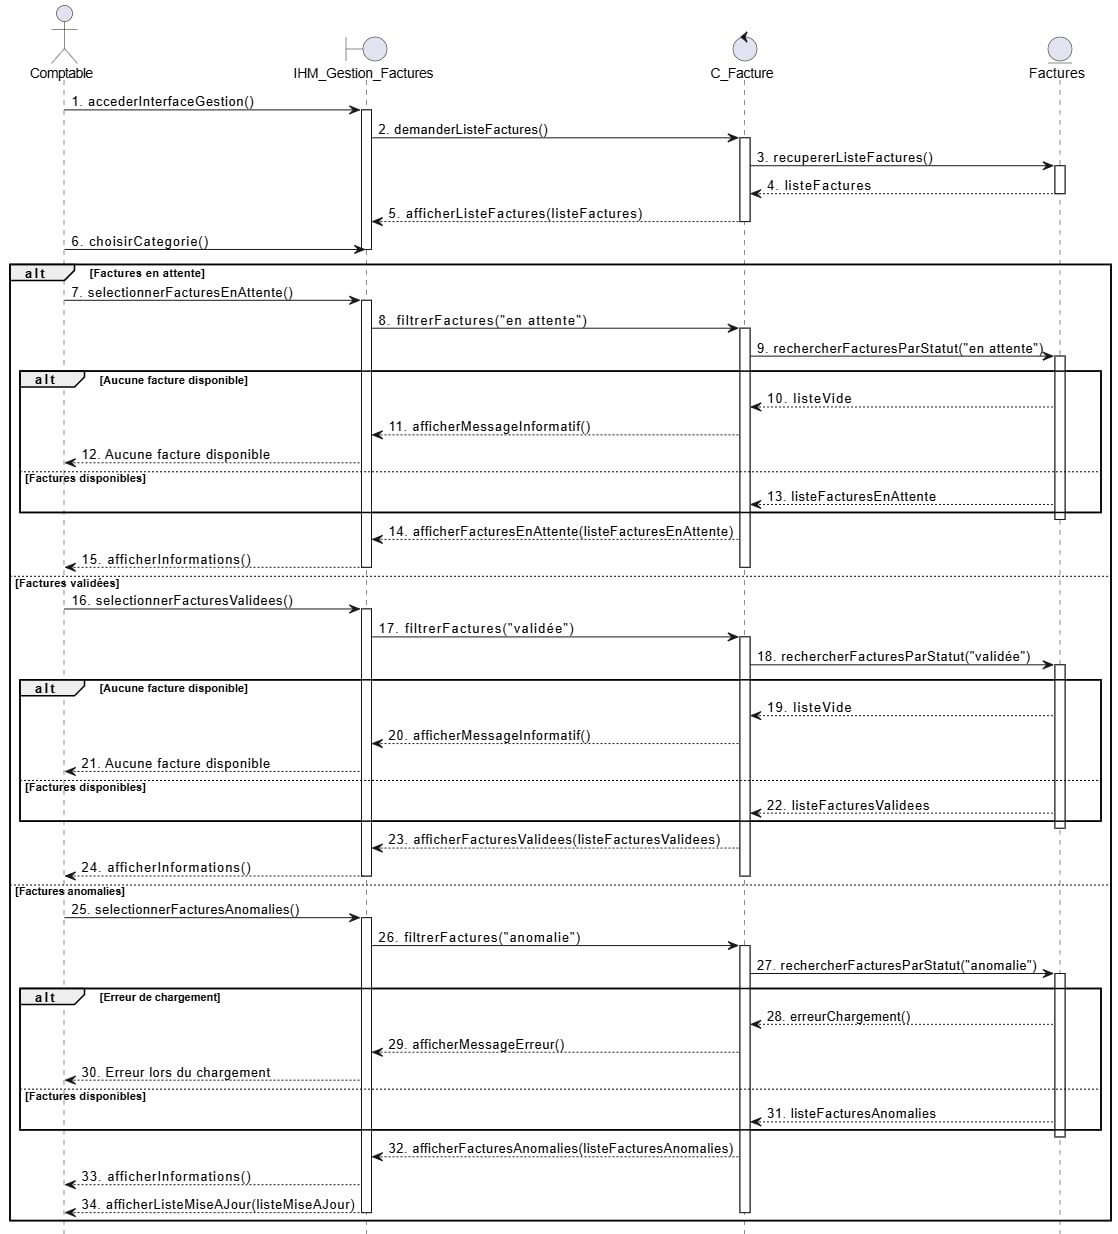
\includegraphics[width=0.65\textwidth]{seq_factures_statut_detail.jpg}
	\caption{Diagramme de séquence détaillé du cas d’utilisation « Gérer les factures »}
	\label{fig:seq_factures_statut_detail}
\end{figure}

\FloatBarrier

%====================================================
\section{Implémentation}

\subsection{Dictionnaire de données}

\subsubsection{Table facture}

\renewcommand{\arraystretch}{1.3}

\begin{table}[H]
	\centering
	\footnotesize
	
	\begin{tabularx}{\textwidth}{|p{3cm}|p{2.5cm}|p{3.5cm}|X|}
		\hline
		
		\rowcolor{blue!20}
		\textbf{Nom du champ}
		&
		\textbf{Type}
		&
		\textbf{Contraintes}
		&
		\textbf{Description}
		\\ \hline
		
		id\_facture
		&
		BIGINT
		&
		PRIMARY KEY
		&
		Identifiant unique de la facture.
		\\ \hline
		
		fournisseur
		&
		VARCHAR
		&
		NOT NULL
		&
		Nom du fournisseur.
		\\ \hline
		
		montant
		&
		FLOAT
		&
		NOT NULL
		&
		Montant total de la facture.
		\\ \hline
		
		dateFacture
		&
		DATE
		&
		NOT NULL
		&
		Date de création de la facture.
		\\ \hline
		
		statut
		&
		VARCHAR
		&
		NOT NULL
		&
		État actuel de la facture.
		\\ \hline
		
	\end{tabularx}
	
	\caption{Dictionnaire de données de la table facture}
	\label{tab:facture_table}
	
\end{table}



\subsubsection{Table dashboard}

\begin{table}[H]
	\centering
	\footnotesize
	
	\begin{tabularx}{\textwidth}{|p{3cm}|p{2.5cm}|p{3.5cm}|X|}
		\hline
		
		\rowcolor{blue!20}
		\textbf{Nom du champ}
		&
		\textbf{Type}
		&
		\textbf{Contraintes}
		&
		\textbf{Description}
		\\ \hline
		
		id\_dashboard
		&
		BIGINT
		&
		PRIMARY KEY
		&
		Identifiant du tableau de bord.
		\\ \hline
		
		nbFactures
		&
		INT
		&
		NOT NULL
		&
		Nombre total des factures.
		\\ \hline
		
		montantTotal
		&
		FLOAT
		&
		NOT NULL
		&
		Somme totale des factures.
		\\ \hline
		
		statistiques
		&
		TEXT
		&
		NULLABLE
		&
		Statistiques affichées dans le dashboard.
		\\ \hline
		
	\end{tabularx}
	
	\caption{Dictionnaire de données de la table dashboard}
	\label{tab:dashboard_table}
	
\end{table}
\section{Réalisation}

\section{Interfaces utilisateur}

\subsubsection{Interface de consultation des résultats d’extraction}

Cette interface permet au comptable de consulter les informations extraites automatiquement des factures après le traitement OCR et IA. Elle affiche les données détectées afin de faciliter leur vérification et leur analyse.

\begin{figure}[H]
	\centering
	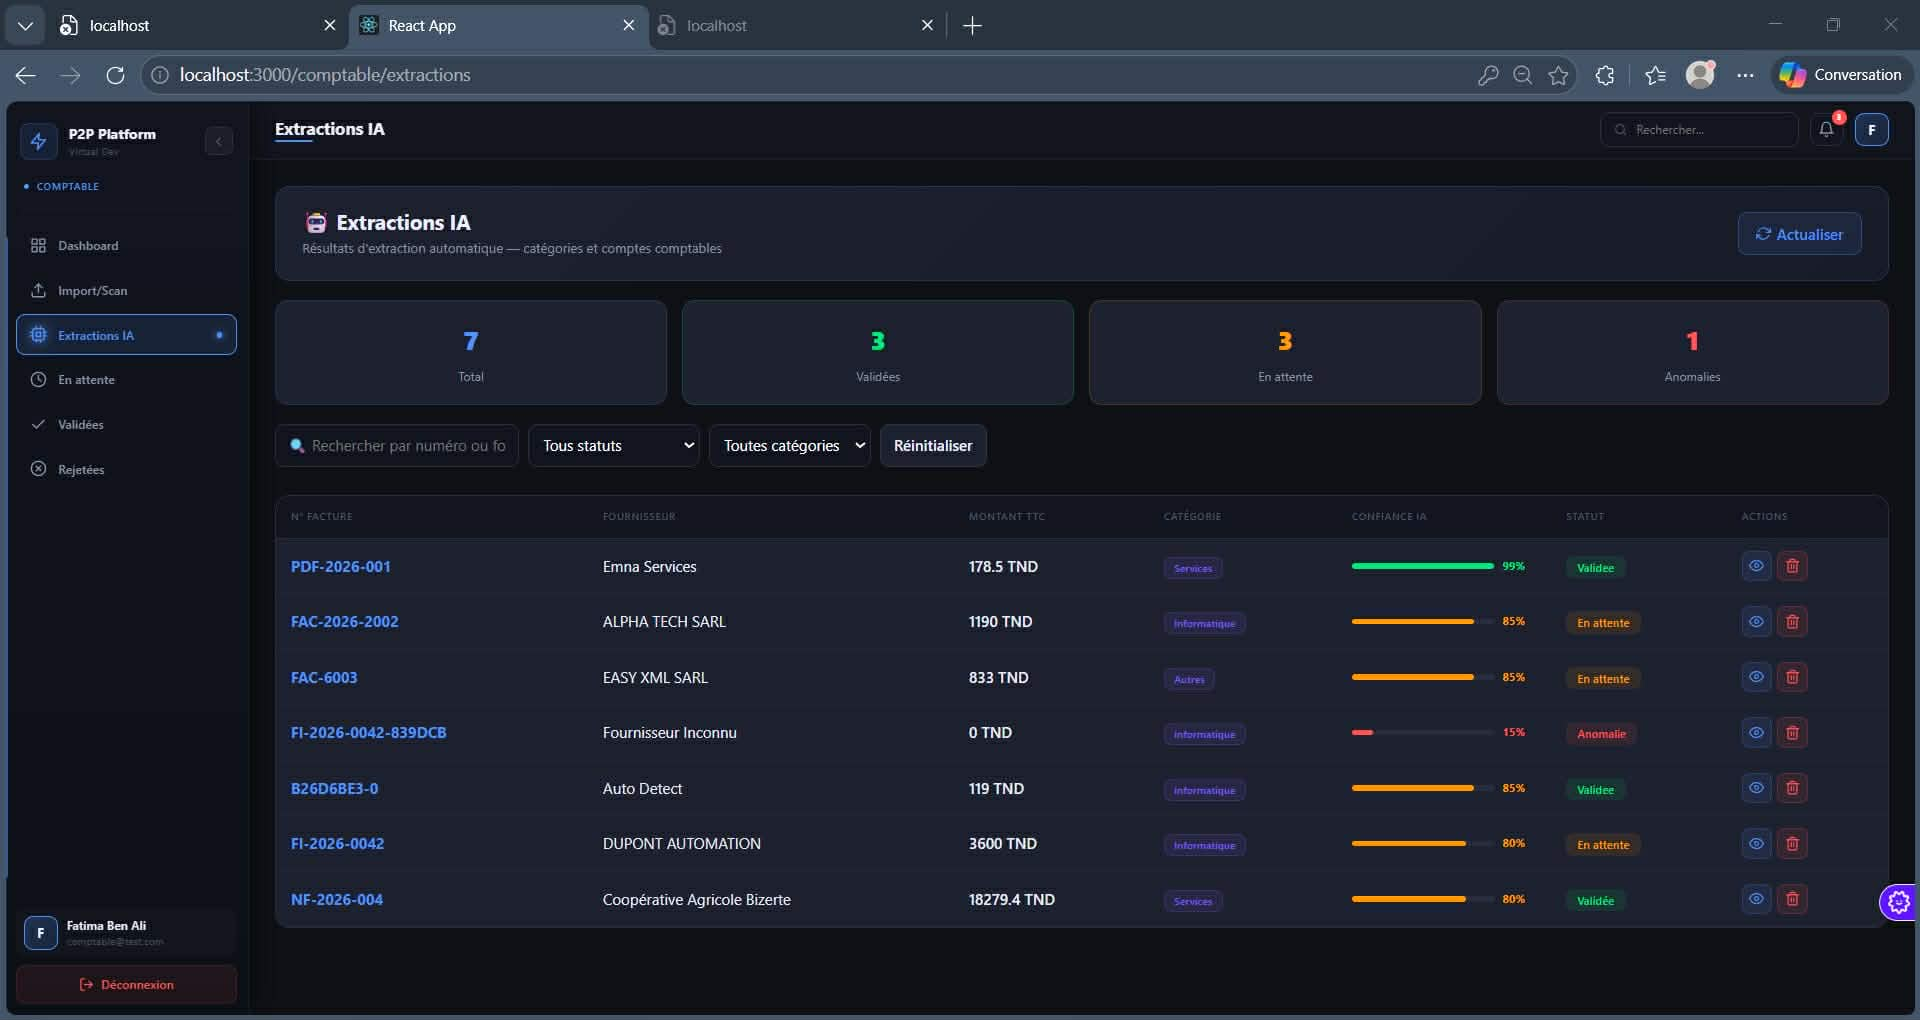
\includegraphics[width=0.85\textwidth]{ui_resultats_extraction.jpg}
	\caption{Interface de consultation des résultats d’extraction}
	\label{fig:ui_resultats_extraction}
\end{figure}

\FloatBarrier

%====================================================
\subsubsection{Interface des factures en attente}

Cette interface affiche les factures en attente de traitement ou de validation. Elle permet au comptable de consulter les factures nécessitant une vérification supplémentaire.

\begin{figure}[H]
	\centering
	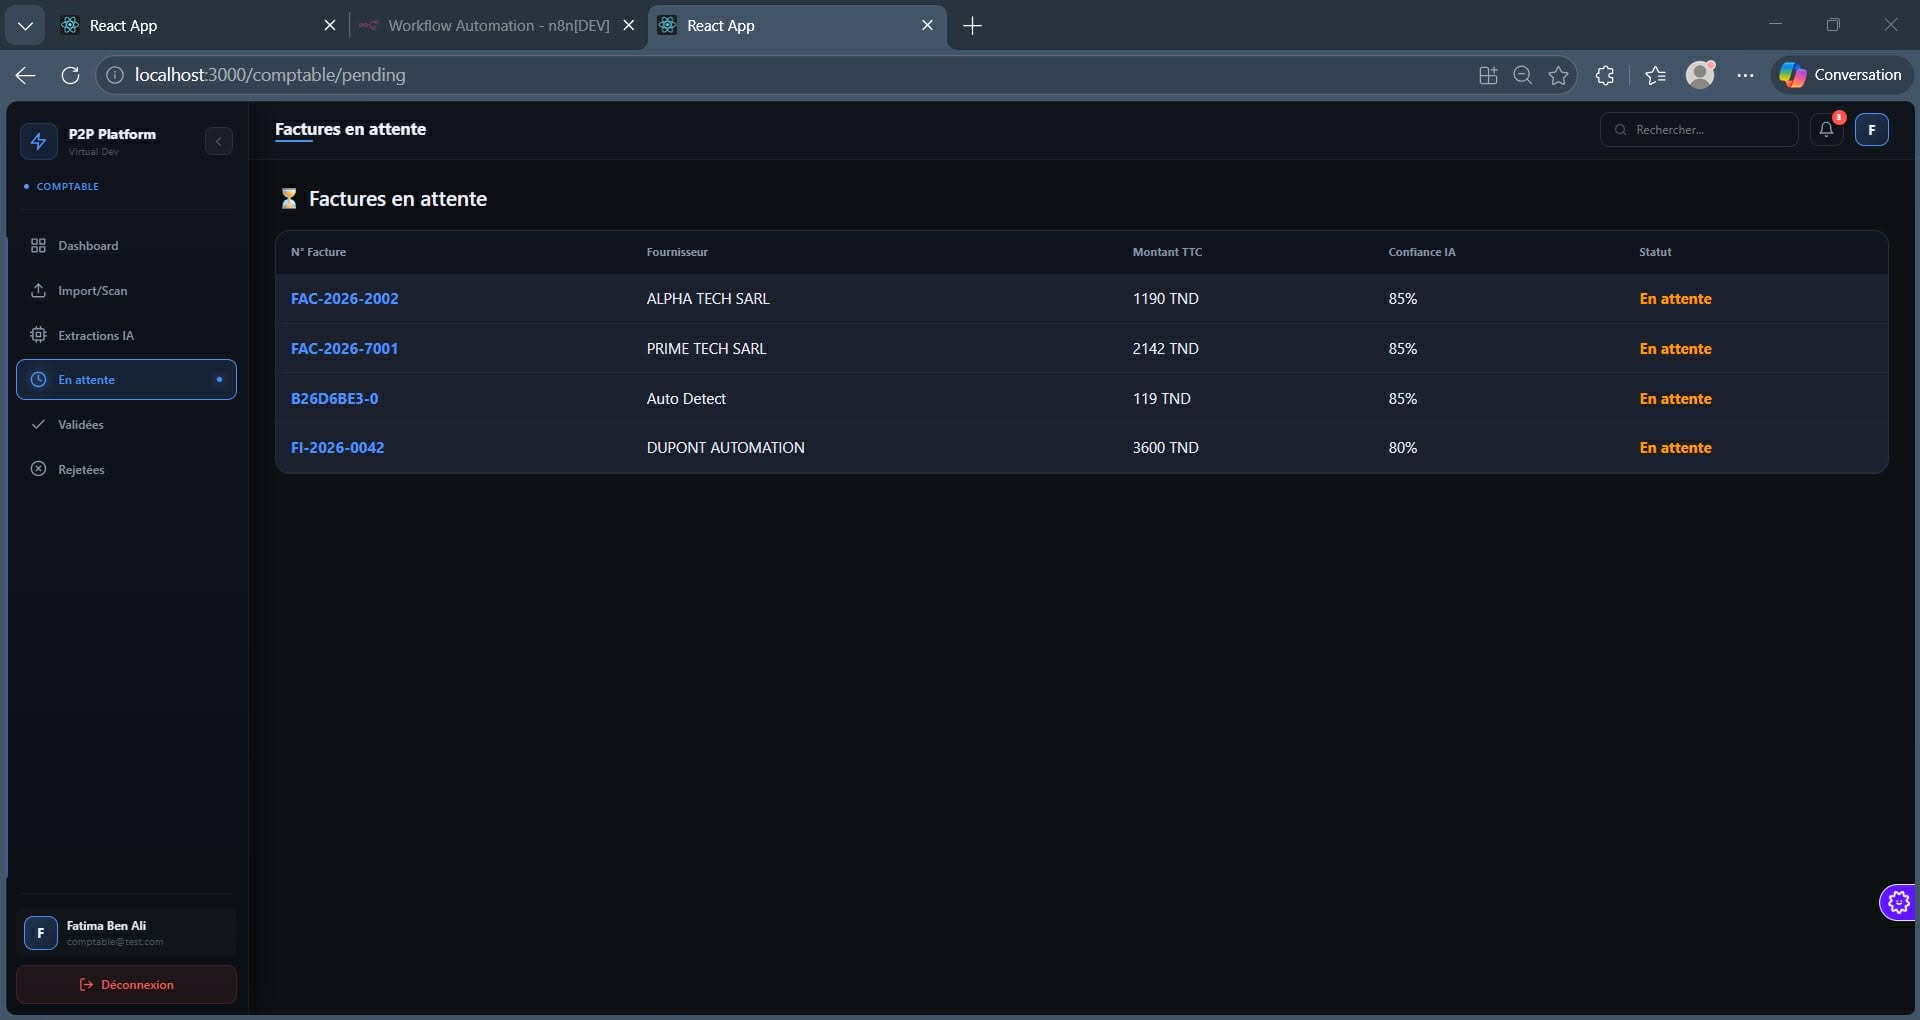
\includegraphics[width=0.85\textwidth]{ui_factures_attente.jpg}
	\caption{Interface des factures en attente}
	\label{fig:ui_factures_attente}
\end{figure}

\FloatBarrier

%====================================================
\subsubsection{Interface des factures validées}

Cette interface présente les factures validées après le processus de contrôle financier. Elle permet de consulter les informations des factures approuvées par le responsable financier.

\begin{figure}[H]
	\centering
	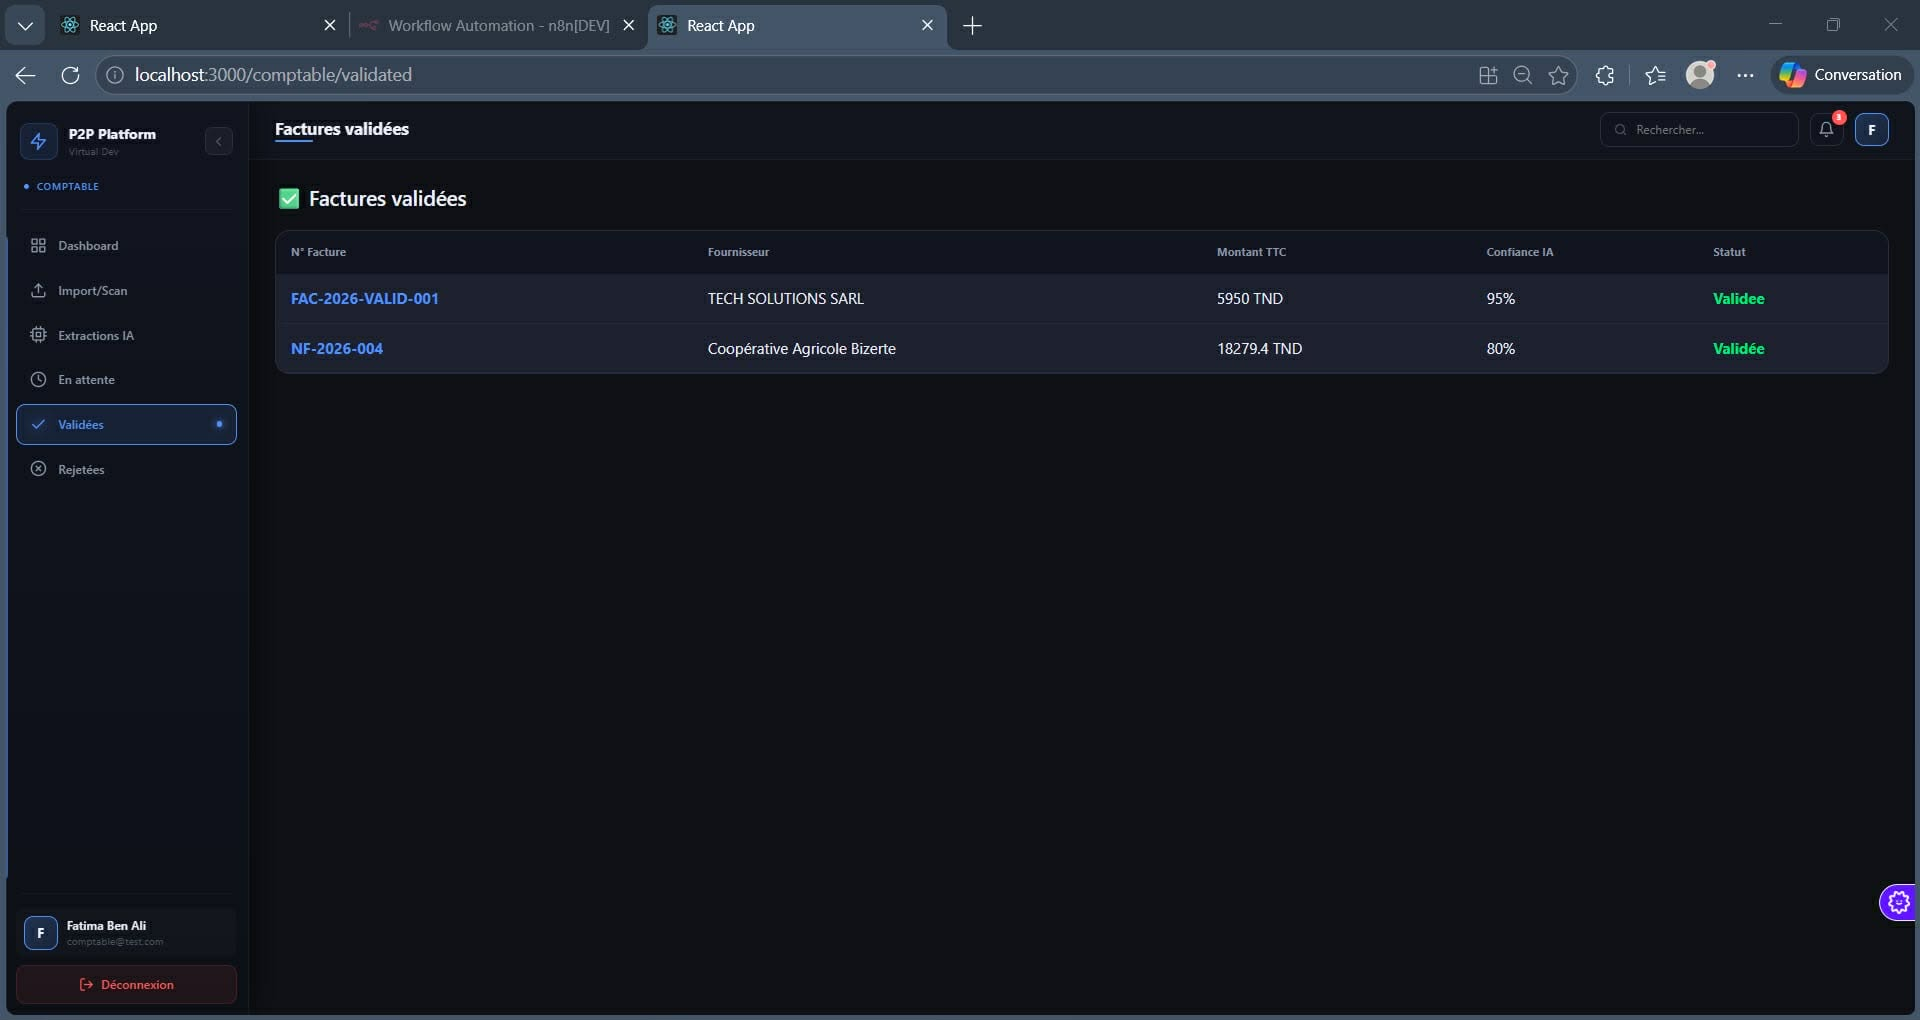
\includegraphics[width=0.85\textwidth]{ui_factures_validees.jpg}
	\caption{Interface des factures validées}
	\label{fig:ui_factures_validees}
\end{figure}

\FloatBarrier

%====================================================
\subsubsection{Interface des factures anomalies}

Cette interface regroupe les factures contenant des anomalies détectées automatiquement par le système. Elle aide les utilisateurs à identifier rapidement les erreurs ou incohérences.

\begin{figure}[H]
	\centering
	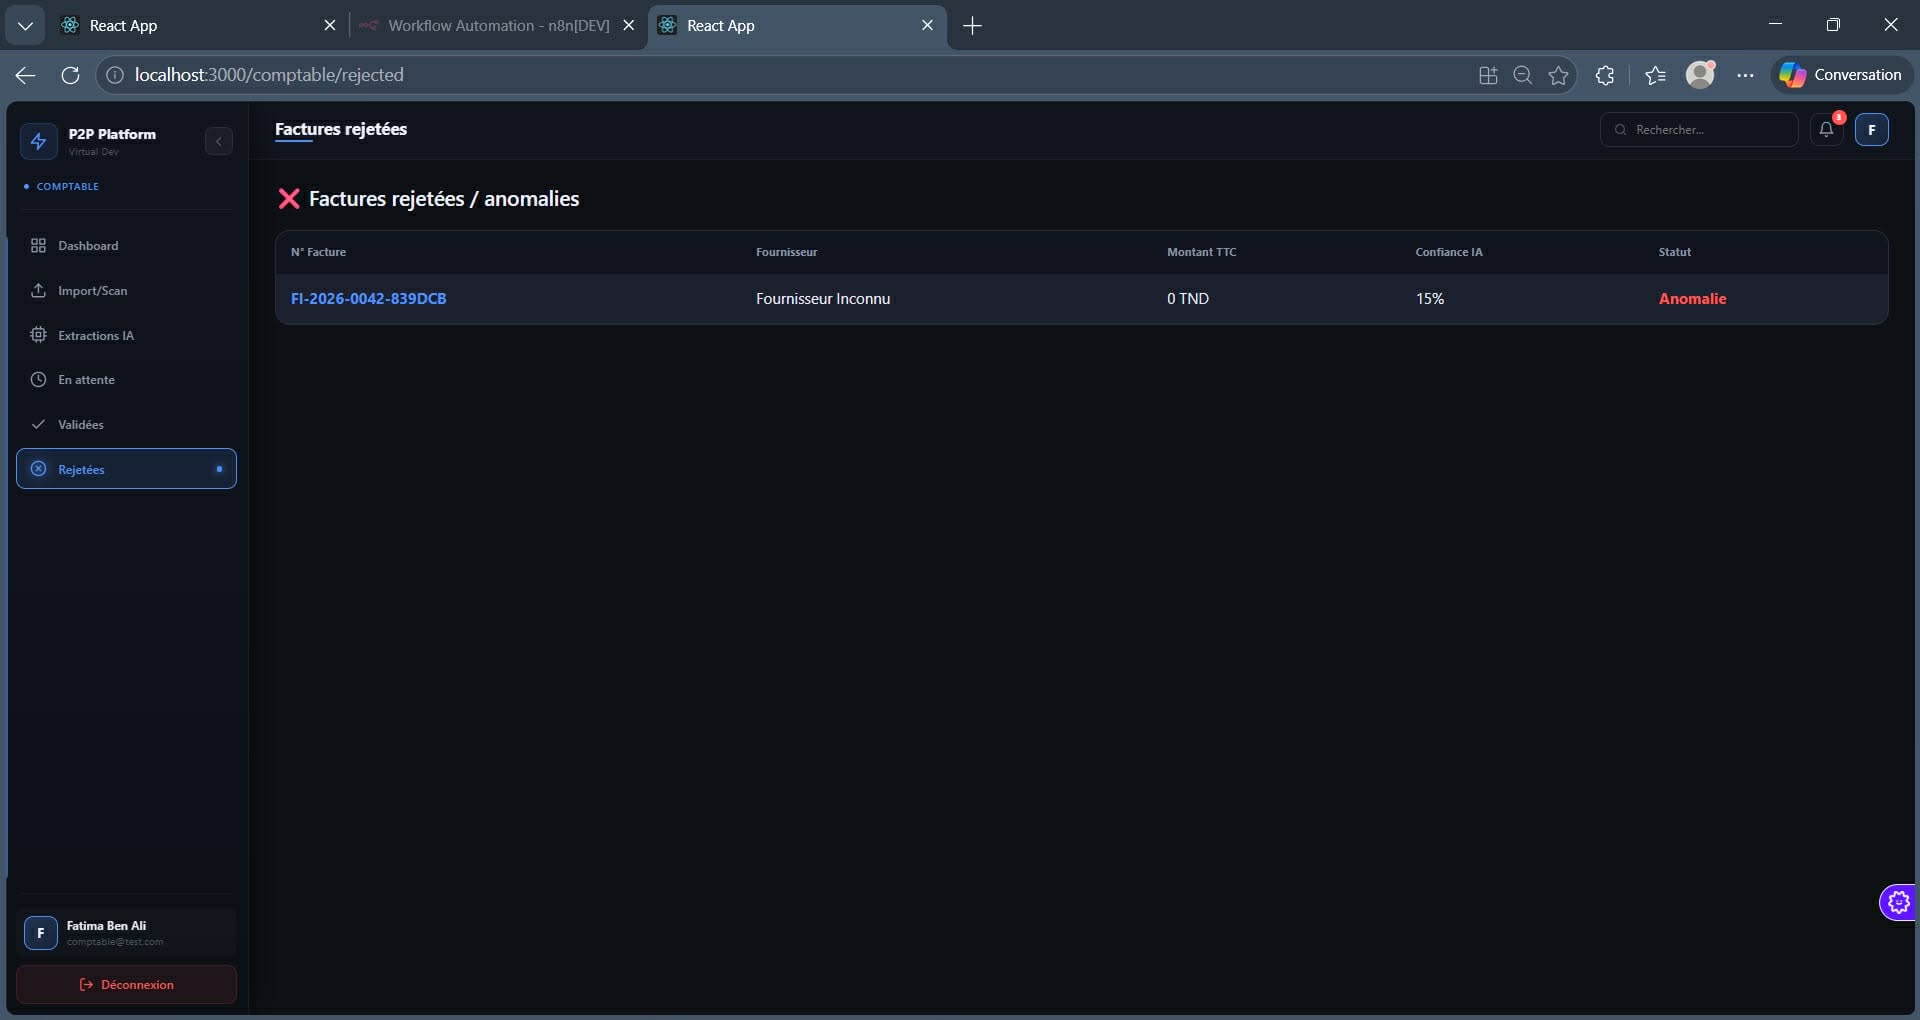
\includegraphics[width=0.85\textwidth]{ui_factures_rejetees.jpg}
	\caption{Interface des factures anomalies}
	\label{fig:ui_factures_anomalies}
\end{figure}

\FloatBarrier

%====================================================
\subsubsection{Interface du tableau de bord}

Cette interface permet de visualiser les statistiques et les indicateurs liés au traitement des factures. Elle offre une vue globale sur les performances et l’état des opérations financières.

\begin{figure}[H]
	\centering
	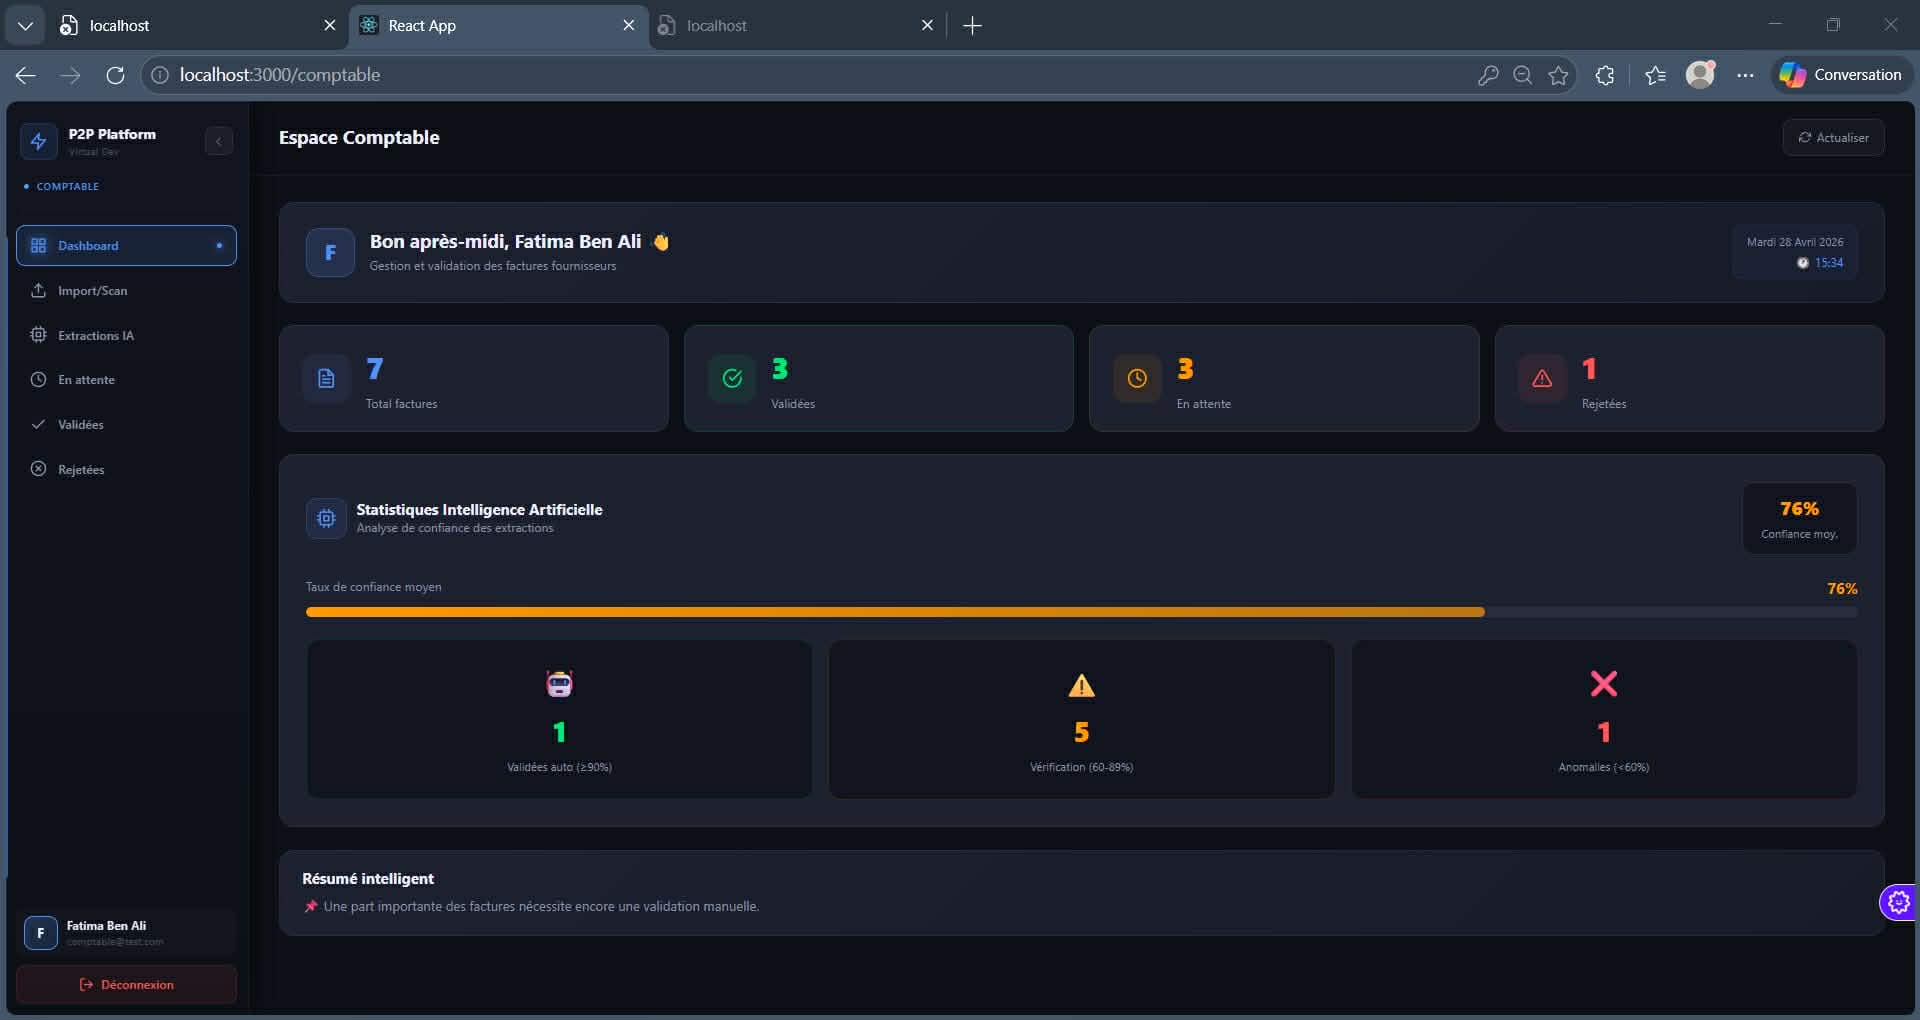
\includegraphics[width=0.85\textwidth]{ui_dashboard.jpg}
	\caption{Interface du tableau de bord}
	\label{fig:ui_dashboard}
\end{figure}

\FloatBarrier

%====================================================
\subsubsection{Interface de configuration des seuils IA}

Cette interface permet à l’administrateur de configurer les seuils de confiance utilisés par l’intelligence artificielle. Elle facilite l’ajustement des paramètres de validation et de détection des anomalies.

\begin{figure}[H]
	\centering
	
\includegraphics[width=0.85\textwidth]{ui_config_ia.jpg}
	\caption{Interface de configuration des seuils IA}
	\label{fig:ui_config_ia}
\end{figure}

\FloatBarrier


\subsection{Tests Postman}

Cette section présente les tests réalisés avec Postman afin de valider les fonctionnalités développées durant le Sprint 2.  
Ces tests concernent principalement l’importation des factures, la consultation des données extraites, la gestion des statuts ainsi que le suivi des actions effectuées dans le système.

Ces tests permettent de vérifier la communication entre le frontend, le backend, la base de données et les services d’analyse des factures.

\renewcommand{\arraystretch}{1.5}

\begin{longtable}{|>{\centering\arraybackslash}m{5cm}|>{\centering\arraybackslash}m{9cm}|}
	\hline
	
	\rowcolor{blue!20}
	\textbf{Description} & \textbf{Capture}
	\\ \hline
	
	Cette requête permet d’importer une facture fournisseur dans le système. 
	Elle permet de tester l’envoi du fichier vers le backend et le déclenchement du processus de traitement automatique.
	&
	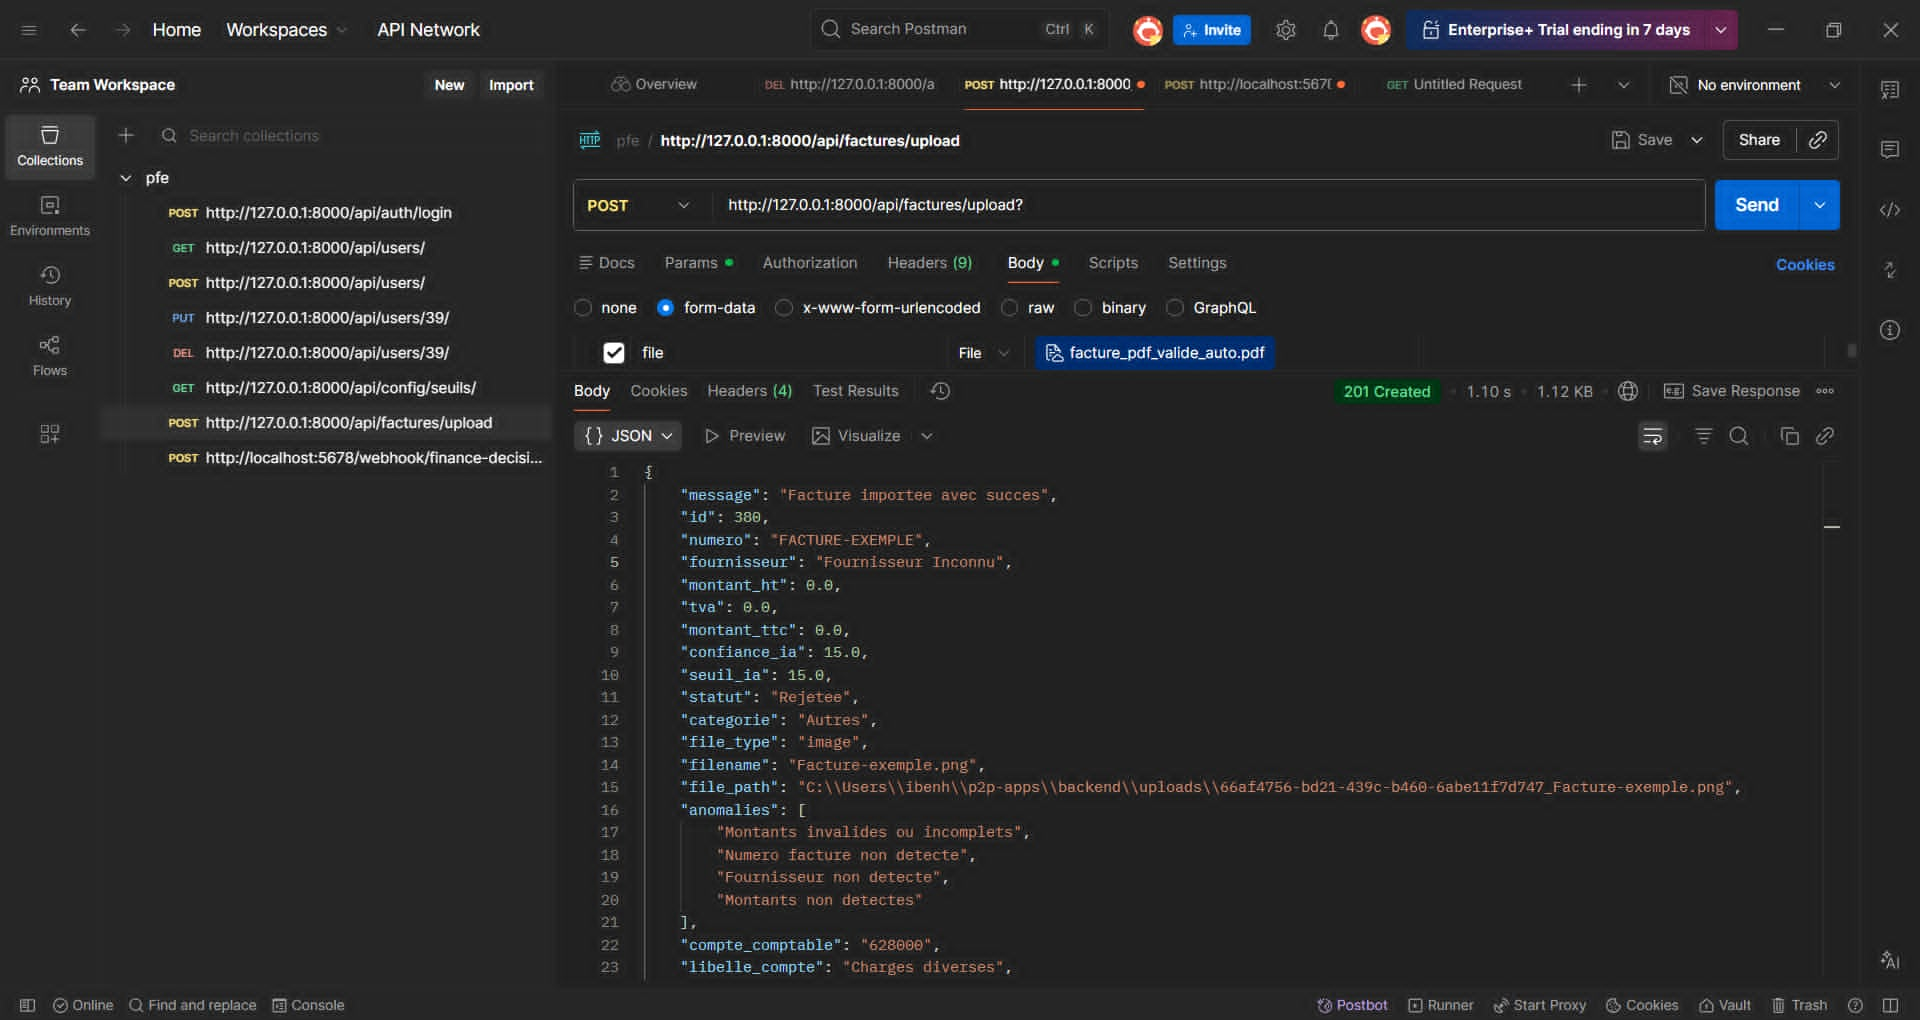
\includegraphics[width=8cm]{figures/postman_import_facture.jpg}
	\\ \hline
	
	Cette requête permet de consulter les données extraites des factures après le traitement OCR et IA. 
	Elle vérifie que les informations détectées sont bien récupérées et affichées correctement.
	&
	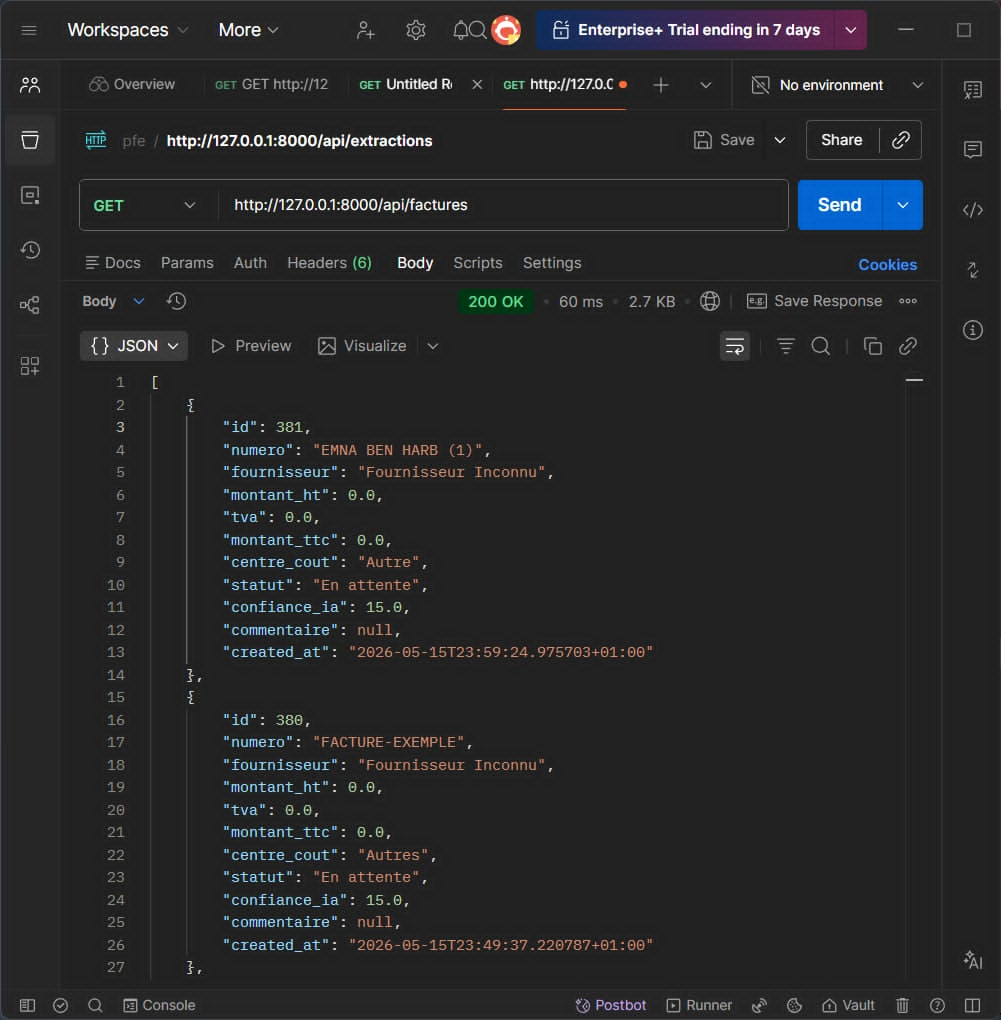
\includegraphics[width=8cm]{figures/postman_resultats.jpg}
	\\ \hline
	
	Cette requête permet de consulter l’historique des actions effectuées dans le système. 
	Elle permet de vérifier la traçabilité des opérations comme l’importation, la modification ou le changement de statut.
	&
	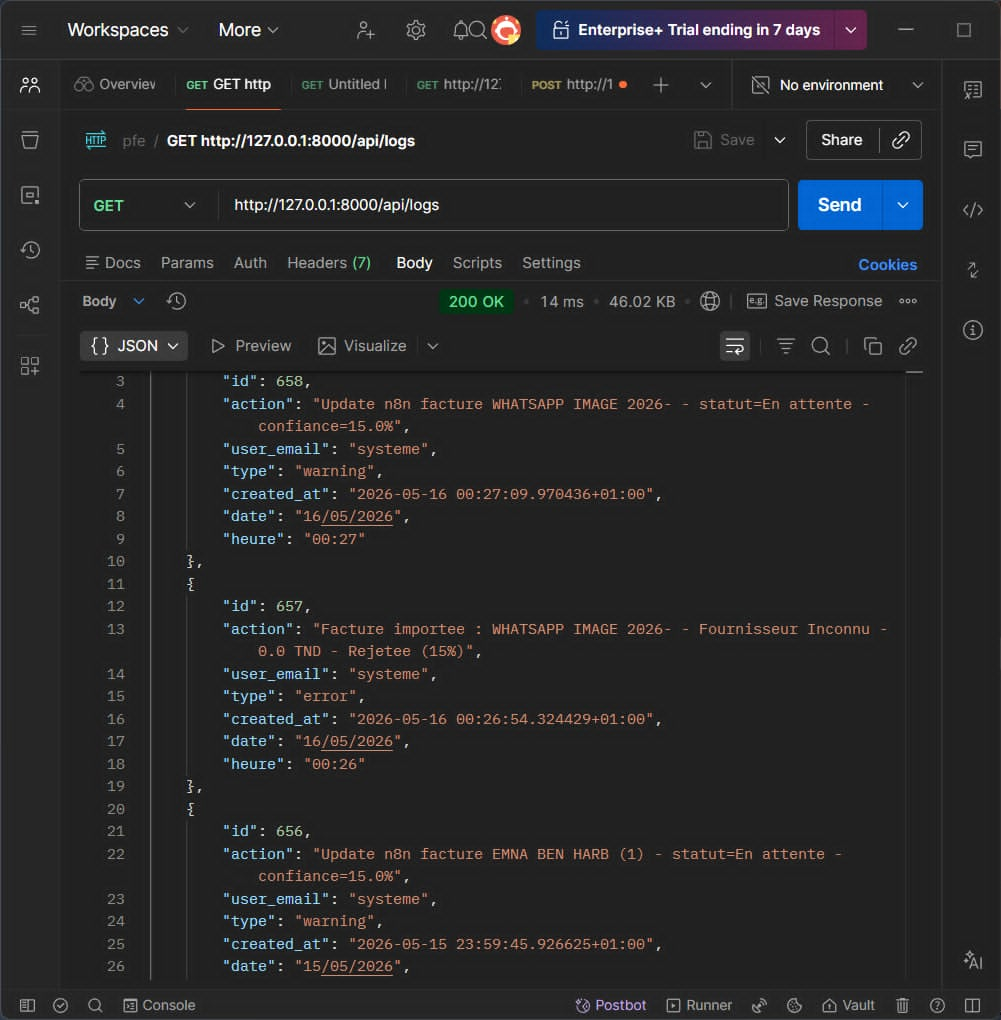
\includegraphics[width=8cm]{figures/postman_logs.jpg}
	\\ \hline
	
	Cette requête permet de récupérer les factures selon leurs statuts. 
	Elle sert à vérifier l’affichage des factures validées, rejetées ou en attente.
	&
	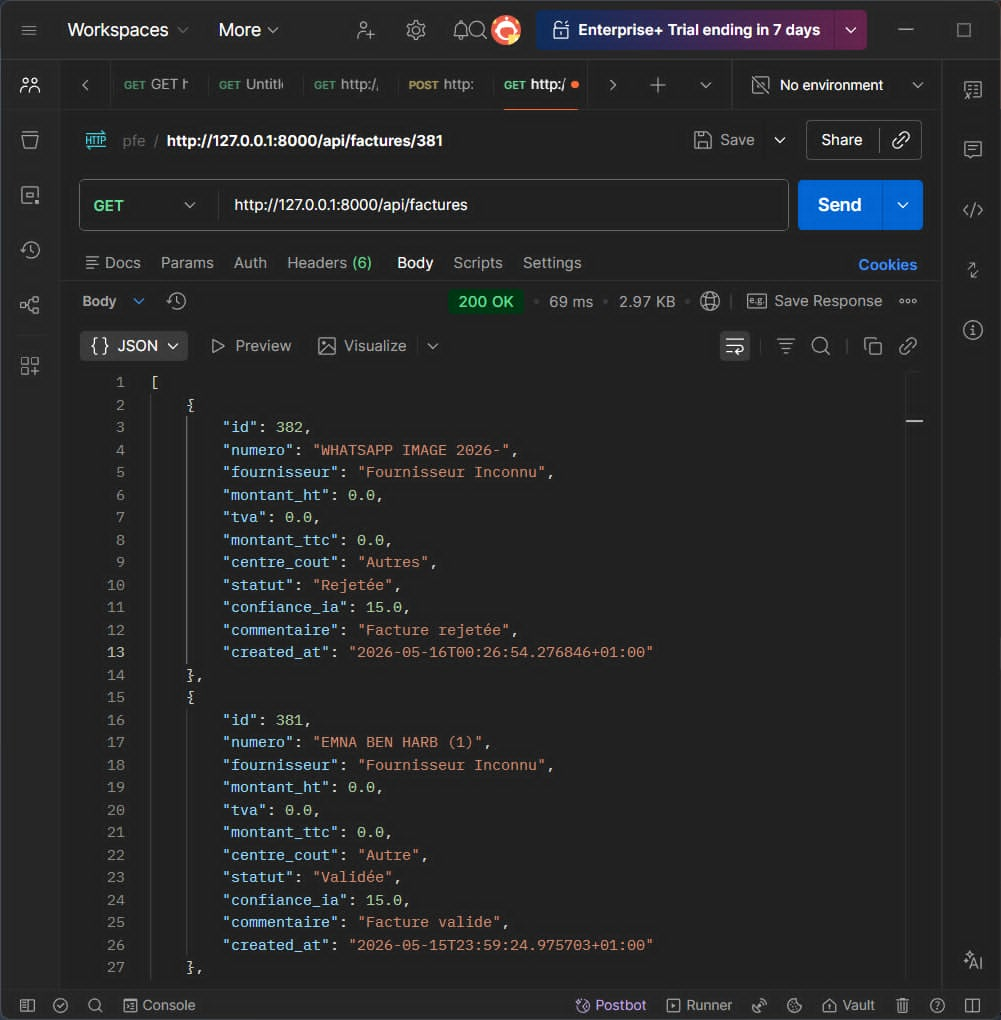
\includegraphics[width=8cm]{figures/postman_factures.jpg}
	\\ \hline
	
	\caption{Tests Postman du Sprint 2}
\end{longtable}
\subsection{Revue de Sprint}

La revue du Sprint 2 a permis de présenter les fonctionnalités développées liées à la gestion des factures, à la consultation des résultats d’extraction ainsi qu’à la visualisation des tableaux de bord et des statistiques. Cette étape a également permis de valider les mécanismes de gestion des statuts
des factures ainsi que la configuration des seuils de confiance de l’intelligence artificielle.
\vspace{0.1cm}
\paragraph{Burndown Chart :}

Le Burndown Chart du Sprint 2 présente l’évolution des tâches relatives au traitement des données, à la consultation des extractions et à la gestion des tableaux de bord. Le graphique illustre la diminution progressive du travail restant jusqu’à la fin du sprint.
Comme présenté dans la figure \ref{fig:brun3}.
\begin{figure}[H]
	\centering
	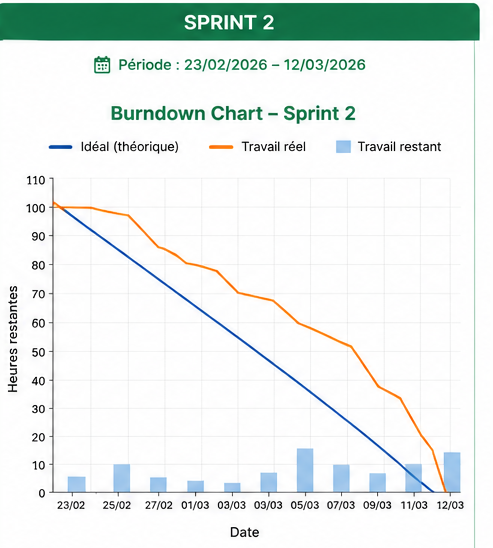
\includegraphics[width=0.4\textwidth]{burndown_sprint2.jpg}
	\caption{Diagramme de Burndown Chart du Sprint 2}
	\label{fig:brun2}
\end{figure}
\begin{table}[H]
	\centering
	\renewcommand{\arraystretch}{1.3}
	
	\begin{tabular}{|c|p{5cm}|c|}
		\hline
		\rowcolor{blue!20}
		\textbf{ID User Story} & \textbf{Fonctionnalité} & \textbf{Estimation} \\
		\hline
		
		2.1 & Consultation des données extraites & 3 \\
		\hline
		
		2.2 & Gestion des statuts des factures & 4 \\
		\hline
		
		2.3 & Tableau de bord comptable & 5 \\
		\hline
		
		2.4 & Gestion des anomalies & 3 \\
		\hline
		
		2.5 & Configuration des seuils IA & 4 \\
		\hline
		
		2.6 & Historique des actions & 2 \\
		\hline
		
		\multicolumn{2}{|c|}{\textbf{Vélocité totale estimée}} & \textbf{21} \\
		\hline
		
	\end{tabular}
	
	\caption{Calcul de vélocité estimée du Sprint 2}
\end{table}
\section{Conclusion}

Dans ce chapitre, nous avons présenté les fonctionnalités développées durant le Sprint 2. Nous avons mis en place la gestion des factures, la consultation des résultats d’extraction, les tableaux de bord ainsi que la configuration des seuils de l’intelligence artificielle.
\chapter{Sprint 3 : Validation et traçabilité}
\newpage
\section{Introduction}


Le cinquième chapitre présente les réalisations du Sprint 3. Nous abordons les fonctionnalités de validation financière, le traitement des anomalies, la gestion des commentaires ainsi que la traçabilité des actions à travers le journal des opérations.


\section{Backlog du Sprint}

\renewcommand{\arraystretch}{1.25}

\begin{table}[H]
	\centering
	\footnotesize
	
	\begin{tabularx}{\textwidth}{|c|p{3.6cm}|c|X|c|}
		\hline
		
		\rowcolor{blue!20}
		\textbf{ID} &
		\textbf{User Story} &
		\textbf{ID-US} &
		\textbf{Tâche} &
		\textbf{Estimation}
		\\ \hline
		
		\multirow{5}{*}{3.1}
		& \multirow{5}{3.6cm}{
			En tant que responsable financier, je veux gérer les validations financières afin de contrôler les factures.
		}
		& 3.1.1 & Conception UML des validations financières. & \multirow{5}{*}{3 jours}
		\\ \cline{3-4}
		
		& & 3.1.2 & Développement de l’interface de validation.
		& \\ \cline{3-4}
		
		& & 3.1.3 & Implémentation des actions approuver/rejeter.
		& \\ \cline{3-4}
		
		& & 3.1.4 & Ajout du système de commentaires obligatoires.
		& \\ \cline{3-4}
		
		& & 3.1.5 & Tests et validation.
		& \\ \hline
		
		\multirow{4}{*}{3.2}
		& \multirow{4}{3.6cm}{
			En tant que responsable financier, je veux voir et modifier les données d’une facture afin de corriger les erreurs détectées.
		}
		& 3.2.1 & Conception UML de consultation et modification. & \multirow{4}{*}{2 jours}
		\\ \cline{3-4}
		
		& & 3.2.2 & Développement de l’interface voir facture.
		& \\ \cline{3-4}
		
		& & 3.2.3 & Développement de l’interface de modification.
		& \\ \cline{3-4}
		
		& & 3.2.4 & Tests et validation.
		& \\ \hline
		
		\multirow{4}{*}{3.3}
		& \multirow{4}{3.6cm}{
			En tant que responsable financier, je veux consulter le tableau de bord financier afin de suivre les opérations financières.
		}
		& 3.3.1 & Conception du tableau de bord financier. & \multirow{4}{*}{2 jours}
		\\ \cline{3-4}
		
		& & 3.3.2 & Développement des graphiques et indicateurs.
		& \\ \cline{3-4}
		
		& & 3.3.3 & Intégration des statistiques dynamiques.
		& \\ \cline{3-4}
		
		& & 3.3.4 & Tests et validation.
		& \\ \hline
		
		\multirow{4}{*}{3.4}
		& \multirow{4}{3.6cm}{
			En tant qu’administrateur, je veux consulter le journal des actions afin d’assurer la traçabilité des opérations.
		}
		& 3.4.1 & Conception UML du journal des actions. & \multirow{4}{*}{1 jour}
		\\ \cline{3-4}
		
		& & 3.4.2 & Développement de l’interface du journal.
		& \\ \cline{3-4}
		
		& & 3.4.3 & Implémentation du stockage des actions.
		& \\ \cline{3-4}
		
		& & 3.4.4 & Tests et validation.
		& \\ \hline
		
	\end{tabularx}
	
	\caption{Backlog détaillé du Sprint 3}
	\label{tab:backlog_sprint3}
	
\end{table}

\FloatBarrier



\section{Analyse}

\subsection{Analyse fonctionnelle}

\subsubsection{Diagramme de cas d’utilisation}

Le diagramme de cas d’utilisation montre les fonctions du troisième sprint. Le diagramme montre le responsable financier qui valide les factures et qui consulte le tableau de bord financier. Le diagramme montre aussi l’administrateur qui consulte le journal des actions.

\begin{figure}[H]
	\centering
	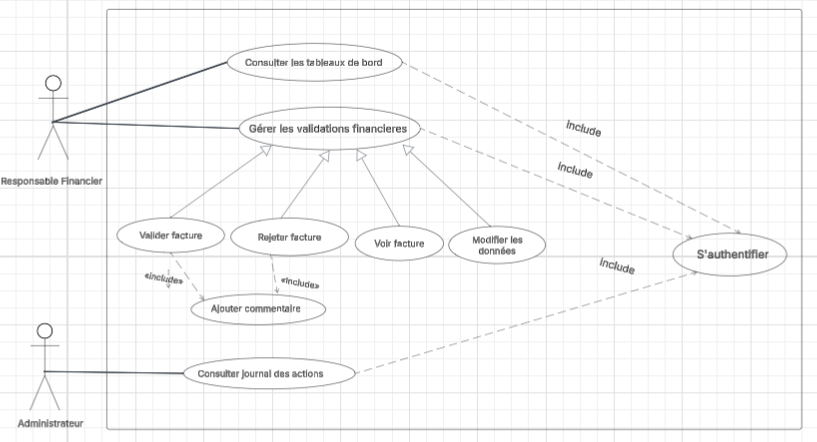
\includegraphics[width=0.9\textwidth]{usecase_sprint3.jpg}
	\caption{Diagramme de cas d’utilisation du Sprint 3}
	\label{fig:usecase_sprint3}
\end{figure}

\FloatBarrier

\subsubsection{Description textuelle des cas d’utilisation}

\subsubsection*{Cas d’utilisation : Gérer les validations financières}

\begin{table}[H]
	\centering
	\renewcommand{\arraystretch}{1.5}
	\small
	\begin{tabularx}{\textwidth}{|p{4.5cm}|X|}
		\hline
		\rowcolor{blue!20}
		\textbf{Nom du cas d’utilisation} & Gérer les validations financières \\ \hline
		
		\textbf{Description brève} & Le responsable financier consulte les détails d’une facture, peut voir le document original, modifier les données si nécessaire, puis approuver ou rejeter la facture avec un commentaire obligatoire. \\ \hline
		
		\textbf{Acteurs primaires} & Responsable financier \\ \hline
		
		\textbf{Acteurs secondaires} & Aucun \\ \hline
		
		\textbf{Pré-condition} & Le responsable financier doit être authentifié. \\ \hline
		
		\textbf{Scénario nominal} &
		1- Le responsable financier ouvre l’interface des validations. \newline
		2- Le système affiche les factures en attente. \newline
		3- Le responsable financier clique sur le bouton « Détails ». \newline
		4- Le système affiche les informations détaillées de la facture. \newline
		5- Si le responsable financier choisit « Voir facture » : \newline
		\hspace*{0.5cm}5.1- Le système affiche le document original de la facture. \newline
		6- Si le responsable financier choisit « Modifier » : \newline
		\hspace*{0.5cm}6.1- Le système active le mode modification. \newline
		\hspace*{0.5cm}6.2- Le responsable financier modifie les données nécessaires. \newline
		\hspace*{0.5cm}6.3- Le système vérifie et enregistre les modifications. \newline
		7- Si le responsable financier choisit « Approuver » : \newline
		\hspace*{0.5cm}7.1- Le responsable financier saisit un commentaire obligatoire. \newline
		\hspace*{0.5cm}7.2- Le système valide la facture. \newline
		\hspace*{0.5cm}7.3- Le système enregistre l’action dans le journal. \newline
		8- Si le responsable financier choisit « Rejeter » : \newline
		\hspace*{0.5cm}8.1- Le responsable financier saisit un commentaire obligatoire. \newline
		\hspace*{0.5cm}8.2- Le système rejette la facture. \newline
		\hspace*{0.5cm}8.3- Le système enregistre l’action dans le journal. \\ \hline
		
		\textbf{Post-condition} & La facture est modifiée si nécessaire, puis validée ou rejetée avec une action enregistrée dans le journal. \\ \hline
		
		\textbf{Scénarios alternatifs} &
		1- Commentaire non saisi. \newline
		1.1- Le système bloque l’approbation ou le rejet. \newline
		2- Données modifiées invalides. \newline
		2.1- Le système refuse l’enregistrement. \newline
		3- Facture introuvable. \newline
		3.1- Le système annule l’opération. \\ \hline
		
	\end{tabularx}
	\caption{Description textuelle du cas d’utilisation « Gérer les validations financières »}
	\label{tab:validation_financiere}
\end{table}

\FloatBarrier

\subsubsection*{Cas d’utilisation : Consulter le journal des actions}

\begin{table}[H]
	\centering
	\renewcommand{\arraystretch}{1.35}
	\rowcolors{2}{gray!10}{white}
	\begin{tabularx}{\textwidth}{|p{3.8cm}|X|}
		\hline
		\rowcolor{blue!20}
		\textbf{Use Case} & Consulter le journal des actions \\ \hline
		
		\textbf{Acteur} & Administrateur \\ \hline
		
		\textbf{Description} & Permet à l’administrateur de consulter l’historique des actions effectuées dans le système afin d’assurer la traçabilité des opérations. \\ \hline
		
		\textbf{Pré-condition} & L’administrateur est authentifié. \\ \hline
		
		\rowcolor{blue!10}
		\textbf{Scénario nominal} &
		1- L’administrateur ouvre l’interface du journal. \newline
		2- Le système récupère les actions qui ont été enregistrées. \newline
		3- Le système affiche la liste des actions. \newline
		4- L’administrateur regarde les informations affichées. \\ \hline
		
		\textbf{Post-condition} & Le journal des actions est affiché. \\ \hline
		
		\rowcolor{blue!10}
		\textbf{Scénarios alternatifs} &
		1- Aucun historique disponible. \newline
		1.1- Le système affiche un message informatif. \newline
		2- Erreur lors du chargement du journal. \newline
		2.1- Le système affiche un message d’erreur. \\ \hline
		
	\end{tabularx}
	\caption{Description textuelle du cas d’utilisation « Consulter le journal des actions »}
	\label{tab:journal_actions}
\end{table}

\FloatBarrier

\subsection{Analyse dynamique}

\subsubsection{Diagramme de séquence système du cas d’utilisation « Gérer les validations financières »}

Le diagramme de séquence système montre les interactions entre le responsable financier et le système. Le diagramme de séquence système décrit le processus d’approbation ou de rejet d’une facture par le responsable financier.

\begin{figure}[H]
	\centering
	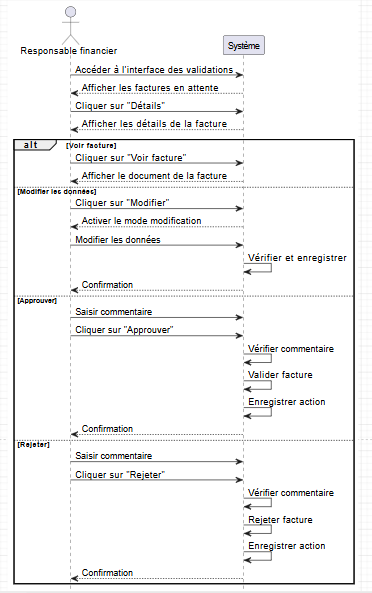
\includegraphics[width=0.85\textwidth]{seq_system_validation.jpg}
	\caption{Diagramme de séquence système - Gérer les validations financières}
	\label{fig:seq_system_validation}
\end{figure}

\FloatBarrier

\subsubsection{Diagramme de séquence système du cas d’utilisation « Consulter le journal des actions »}

Le diagramme suivant montre les interactions entre l’administrateur et le système. L’administrateur consulte le journal des actions.

\begin{figure}[H]
	\centering
	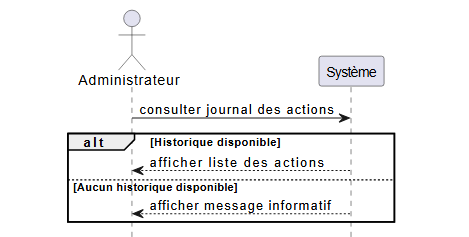
\includegraphics[width=0.85\textwidth]{seq_system_journal.jpg}
	\caption{Diagramme de séquence système - Consulter le journal des actions}
	\label{fig:seq_system_journal}
\end{figure}

\FloatBarrier

\section{Conception}
\subsection{Conception statique}

\subsubsection{Diagramme de classes du Sprint 3}

Le diagramme de classes montre les entités manipulées pendant ce sprint. Il indique les factures, les commentaires liés aux décisions et le journal qui assure la traçabilité des actions.

\begin{figure}[H]
	\centering
	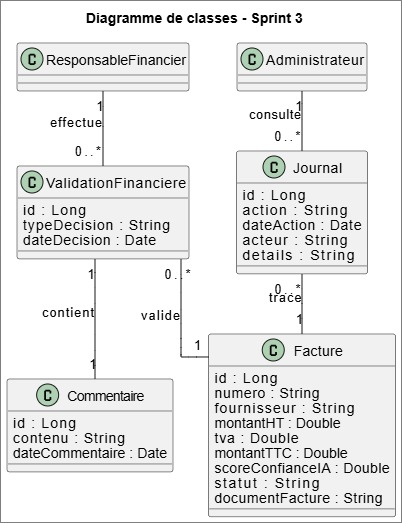
\includegraphics[width=0.85\textwidth]{class_sprint3.jpg}
	\caption{Diagramme de classes du Sprint 3}
	\label{fig:class_sprint3}
\end{figure}

\FloatBarrier
\subsection{Conception dynamique}

\subsubsection{Diagramme de séquence détaillé du cas d’utilisation « Gérer les validations financières »}

Le diagramme suivant montre les interactions entre les différents composants du système lors de l’approbation d’une facture ou du rejet d’une facture. L’ajout d’un commentaire est obligatoire et l’action est enregistrée dans le journal.

\begin{figure}[H]
	\centering
	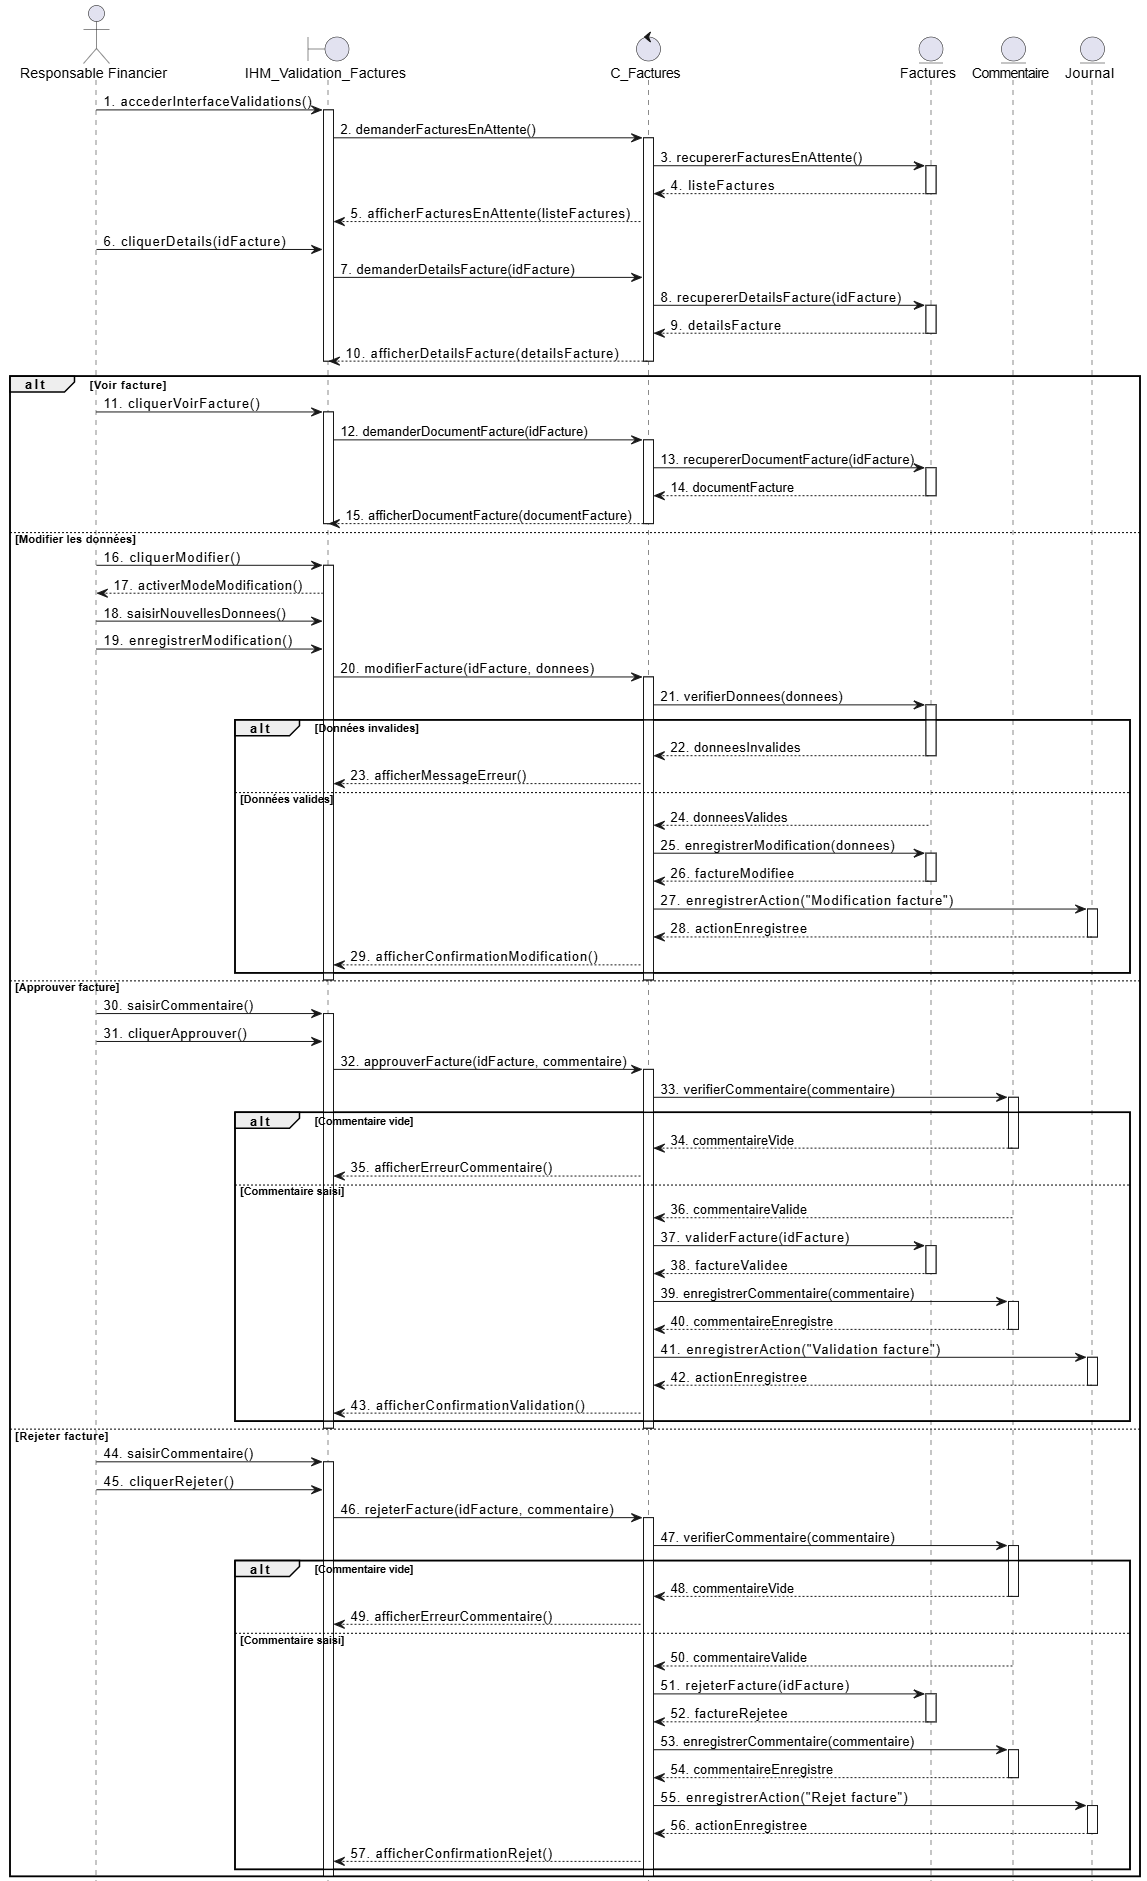
\includegraphics[width=0.85\textwidth]{seq_detail_validation.jpg}
	\caption{Diagramme de séquence détaillé - Gérer les validations financières}
	\label{fig:seq_detail_validation}
\end{figure}

\FloatBarrier

\subsubsection{Diagramme de séquence détaillé du cas d’utilisation « Consulter le journal des actions »}

Le diagramme montre les échanges entre l’administrateur, l’interface du journal, le contrôleur et la base de données lors de la consultation de l’historique des actions.

\begin{figure}[H]
	\centering
	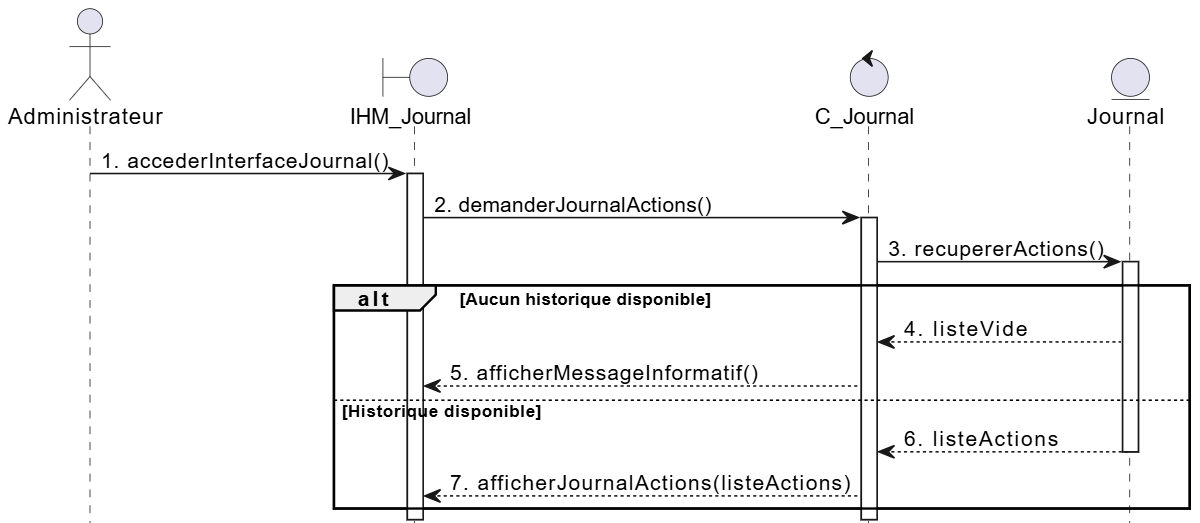
\includegraphics[width=0.85\textwidth]{seq_detail_journal.jpg}
	\caption{Diagramme de séquence détaillé - Consulter le journal des actions}
	\label{fig:seq_detail_journal}
\end{figure}

\FloatBarrier


\section{Implémentation}

\subsection{Dictionnaire de données}

\subsubsection{Table validation}

\renewcommand{\arraystretch}{1.3}

\begin{table}[H]
	\centering
	\footnotesize
	
	\begin{tabularx}{\textwidth}{|p{3cm}|p{2.5cm}|p{3.5cm}|X|}
		\hline
		
		\rowcolor{blue!20}
		\textbf{Nom du champ}
		&
		\textbf{Type}
		&
		\textbf{Contraintes}
		&
		\textbf{Description}
		\\ \hline
		
		id\_validation
		&
		BIGINT
		&
		PRIMARY KEY
		&
		Identifiant unique de la validation.
		\\ \hline
		
		factureId
		&
		BIGINT
		&
		FOREIGN KEY
		&
		Facture concernée par la validation.
		\\ \hline
		
		decision
		&
		VARCHAR
		&
		NOT NULL
		&
		Décision prise sur la facture.
		\\ \hline
		
		commentaire
		&
		TEXT
		&
		NOT NULL
		&
		Commentaire obligatoire ajouté par le responsable.
		\\ \hline
		
		dateValidation
		&
		DATETIME
		&
		NOT NULL
		&
		Date de validation de la facture.
		\\ \hline
		
	\end{tabularx}
	
	\caption{Dictionnaire de données de la table validation}
	\label{tab:validation_table}
	
\end{table}



\subsubsection{Table journal des actions}

\begin{table}[H]
	\centering
	\footnotesize
	
	\begin{tabularx}{\textwidth}{|p{3cm}|p{2.5cm}|p{3.5cm}|X|}
		\hline
		
		\rowcolor{blue!20}
		\textbf{Nom du champ}
		&
		\textbf{Type}
		&
		\textbf{Contraintes}
		&
		\textbf{Description}
		\\ \hline
		
		id\_journal
		&
		BIGINT
		&
		PRIMARY KEY
		&
		Identifiant du journal.
		\\ \hline
		
		utilisateur
		&
		VARCHAR
		&
		NOT NULL
		&
		Nom de l’utilisateur ayant effectué l’action.
		\\ \hline
		
		action
		&
		TEXT
		&
		NOT NULL
		&
		Description de l’action réalisée.
		\\ \hline
		
		dateAction
		&
		DATETIME
		&
		NOT NULL
		&
		Date et heure de l’action.
		\\ \hline
		
	\end{tabularx}
	
	\caption{Dictionnaire de données de la table journal des actions}
	\label{tab:journal_table}
	
\end{table}
\section{Réalisation}

\subsection{Interfaces utilisateur}

\subsubsection{Interface de validation des factures}

Cette interface permet au responsable financier de consulter la liste des factures en attente de décision. Elle affiche les informations principales de chaque facture, telles que le fournisseur, le montant, le score de confiance de l’IA et le statut.

\begin{figure}[H]
	\centering
	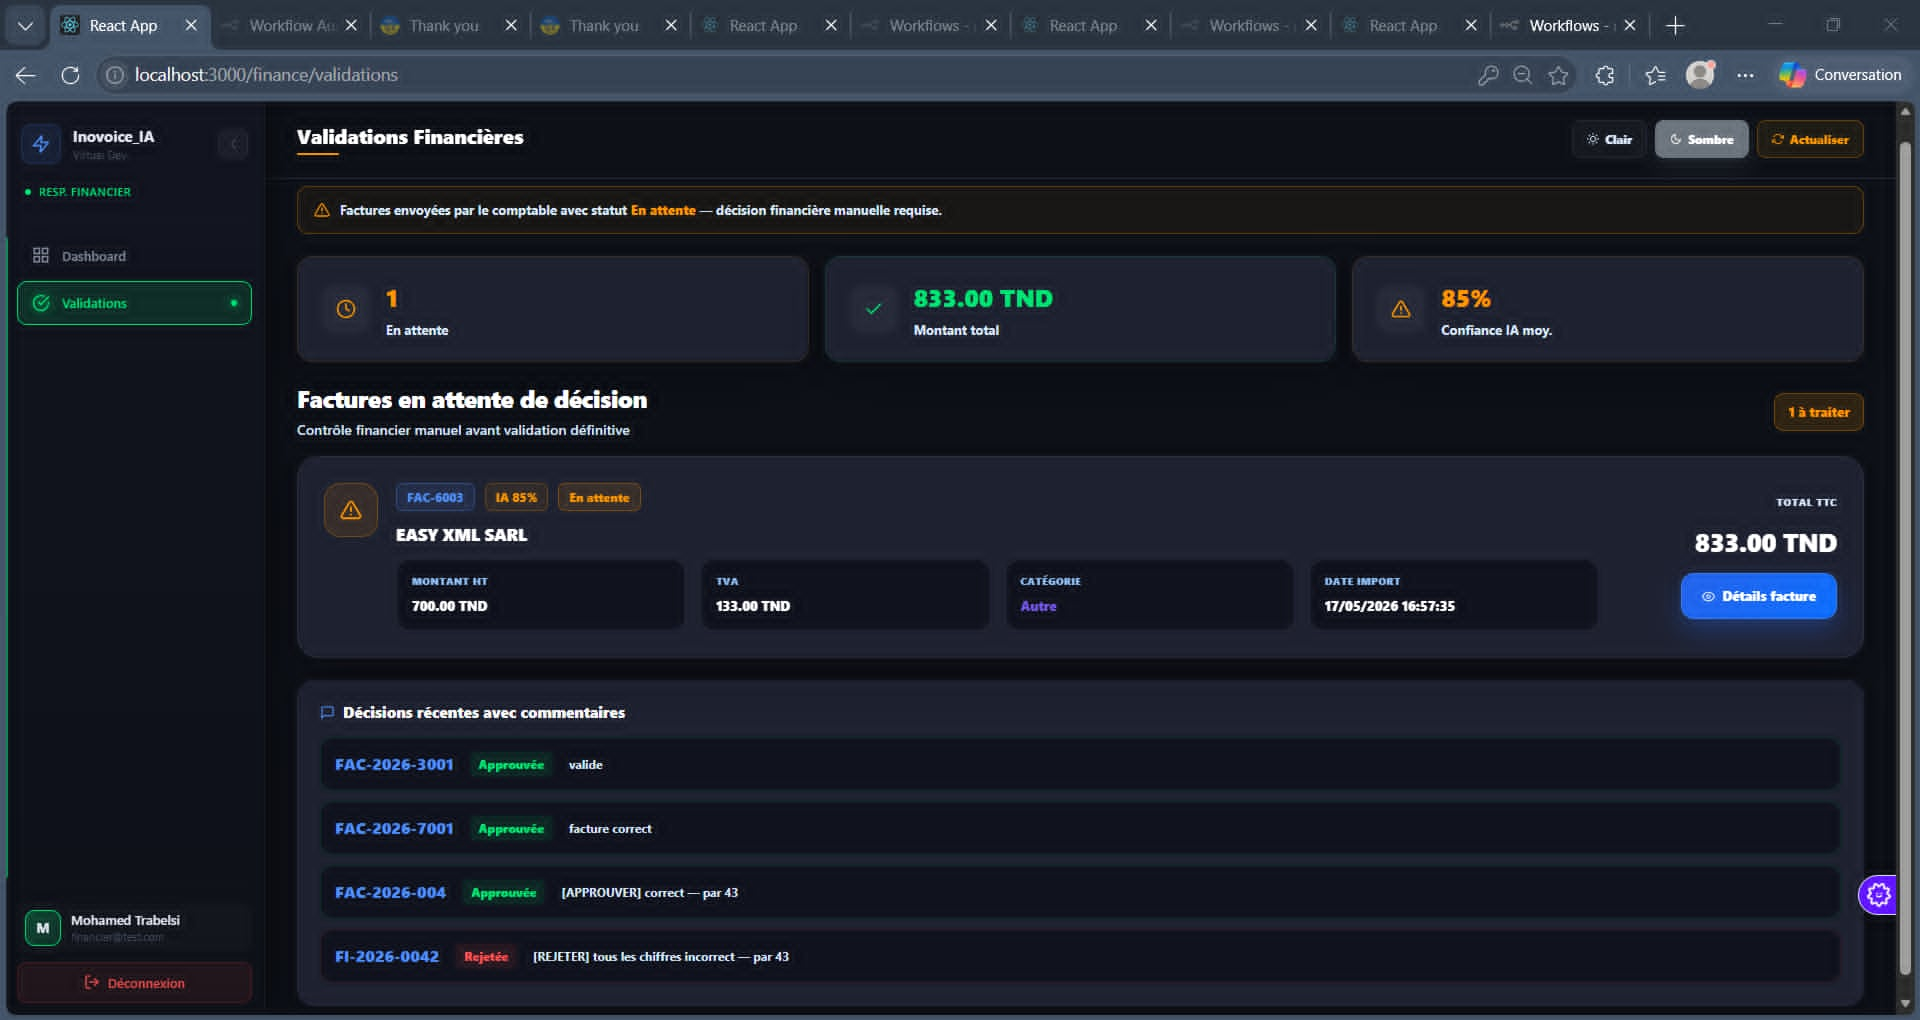
\includegraphics[width=0.85\textwidth]{ui_validation_factures.jpg}
	\caption{Interface de validation des factures}
	\label{fig:ui_validation_factures}
\end{figure}

\FloatBarrier

\subsubsection{Interface des détails de la facture}

Cette interface affiche les informations détaillées de la facture sélectionnée. Elle permet au responsable financier de vérifier les données extraites, de consulter le document original, de modifier les données si nécessaire, puis d’approuver ou de rejeter la facture avec un commentaire obligatoire.

\begin{figure}[H]
	\centering
	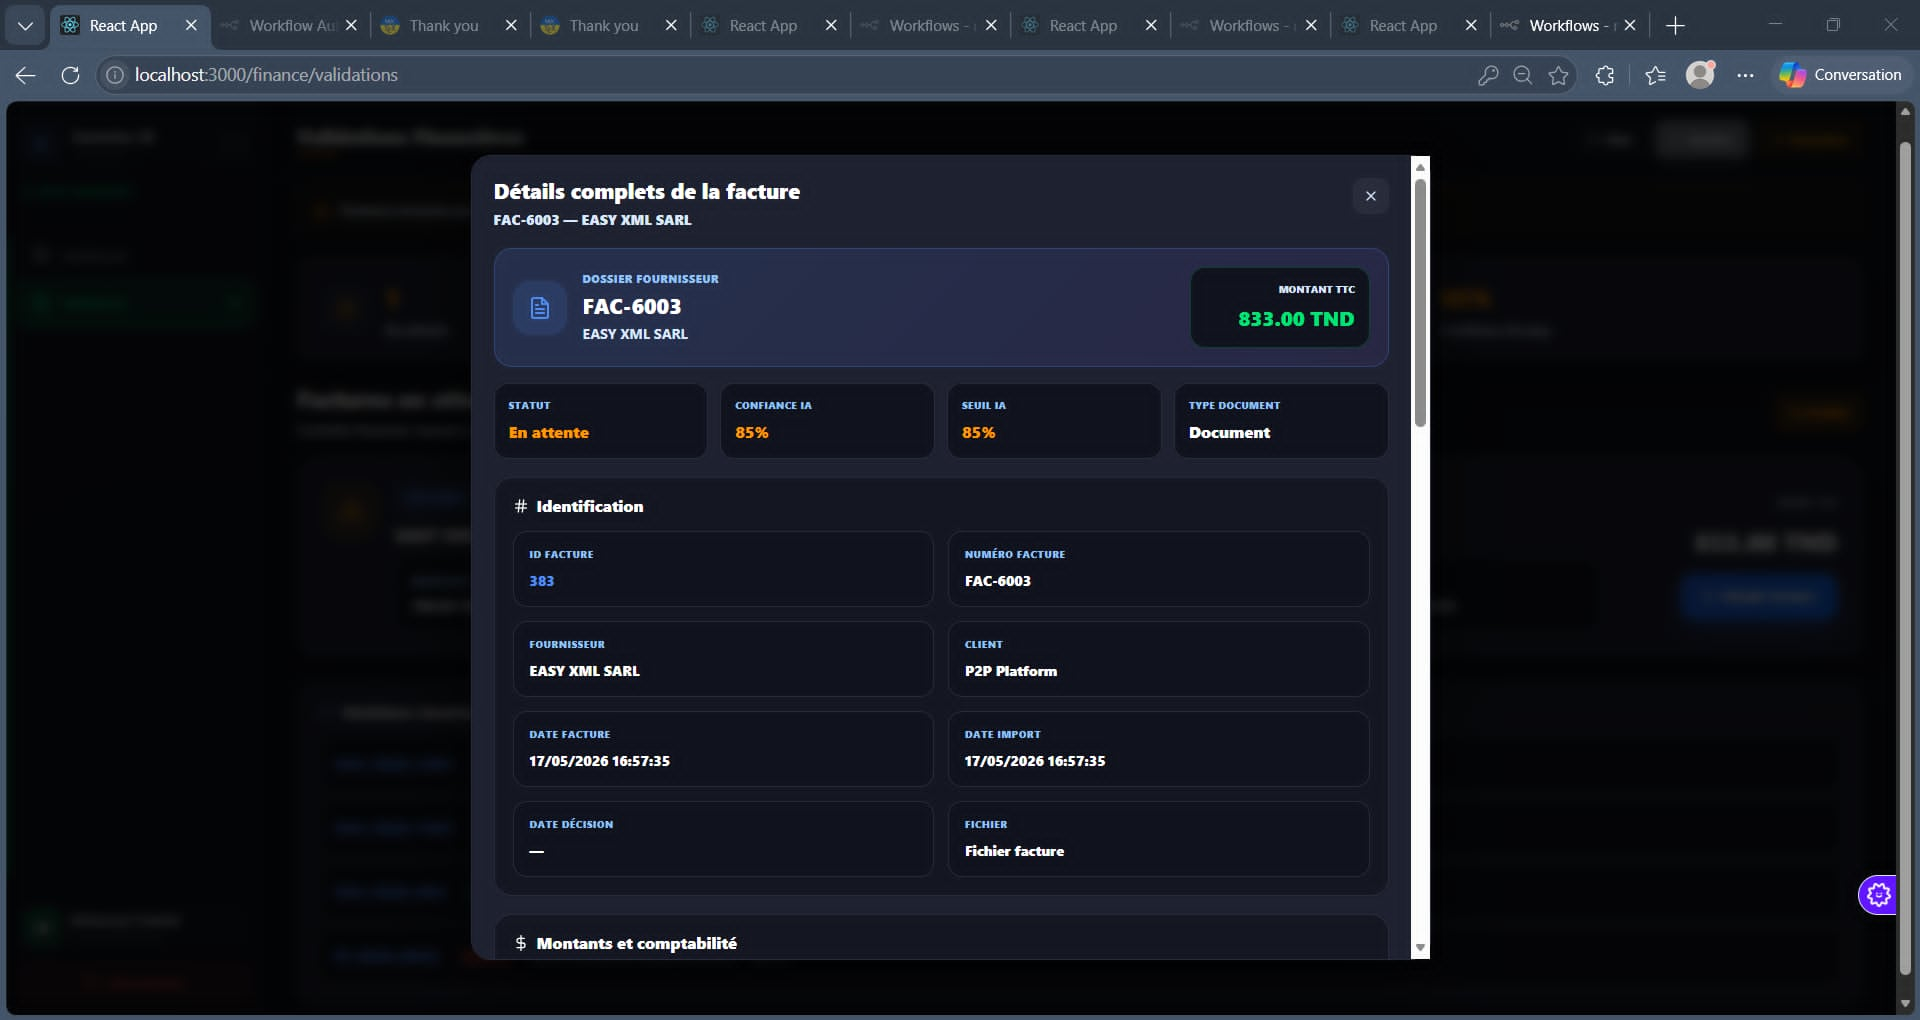
\includegraphics[width=0.85\textwidth]{ui_details_facture.jpg}
	\caption{Interface des détails de la facture}
	\label{fig:ui_details_facture}
\end{figure}

\FloatBarrier

\subsubsection{Interface de modification des données de la facture}

Cette interface permet au responsable financier de corriger les données extraites automatiquement lorsqu’une erreur est détectée.

\begin{figure}[H]
	\centering
	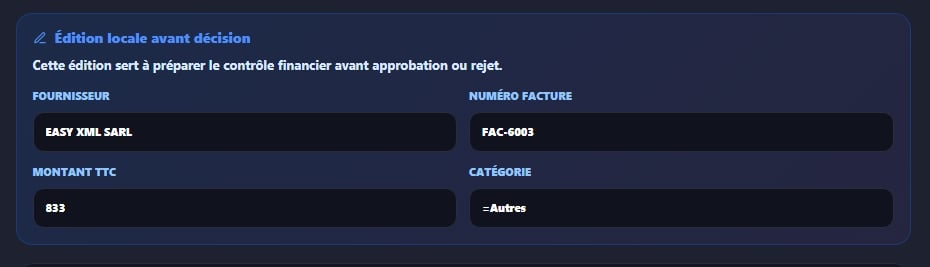
\includegraphics[width=0.85\textwidth]{ui_modifier_facture.jpg}
	\caption{Interface de modification des données de la facture}
	\label{fig:ui_modifier_facture}
\end{figure}

\FloatBarrier

\subsubsection{Interface du commentaire obligatoire}

Cette interface permet au responsable financier de saisir un commentaire avant toute décision finale.

\begin{figure}[H]
	\centering
	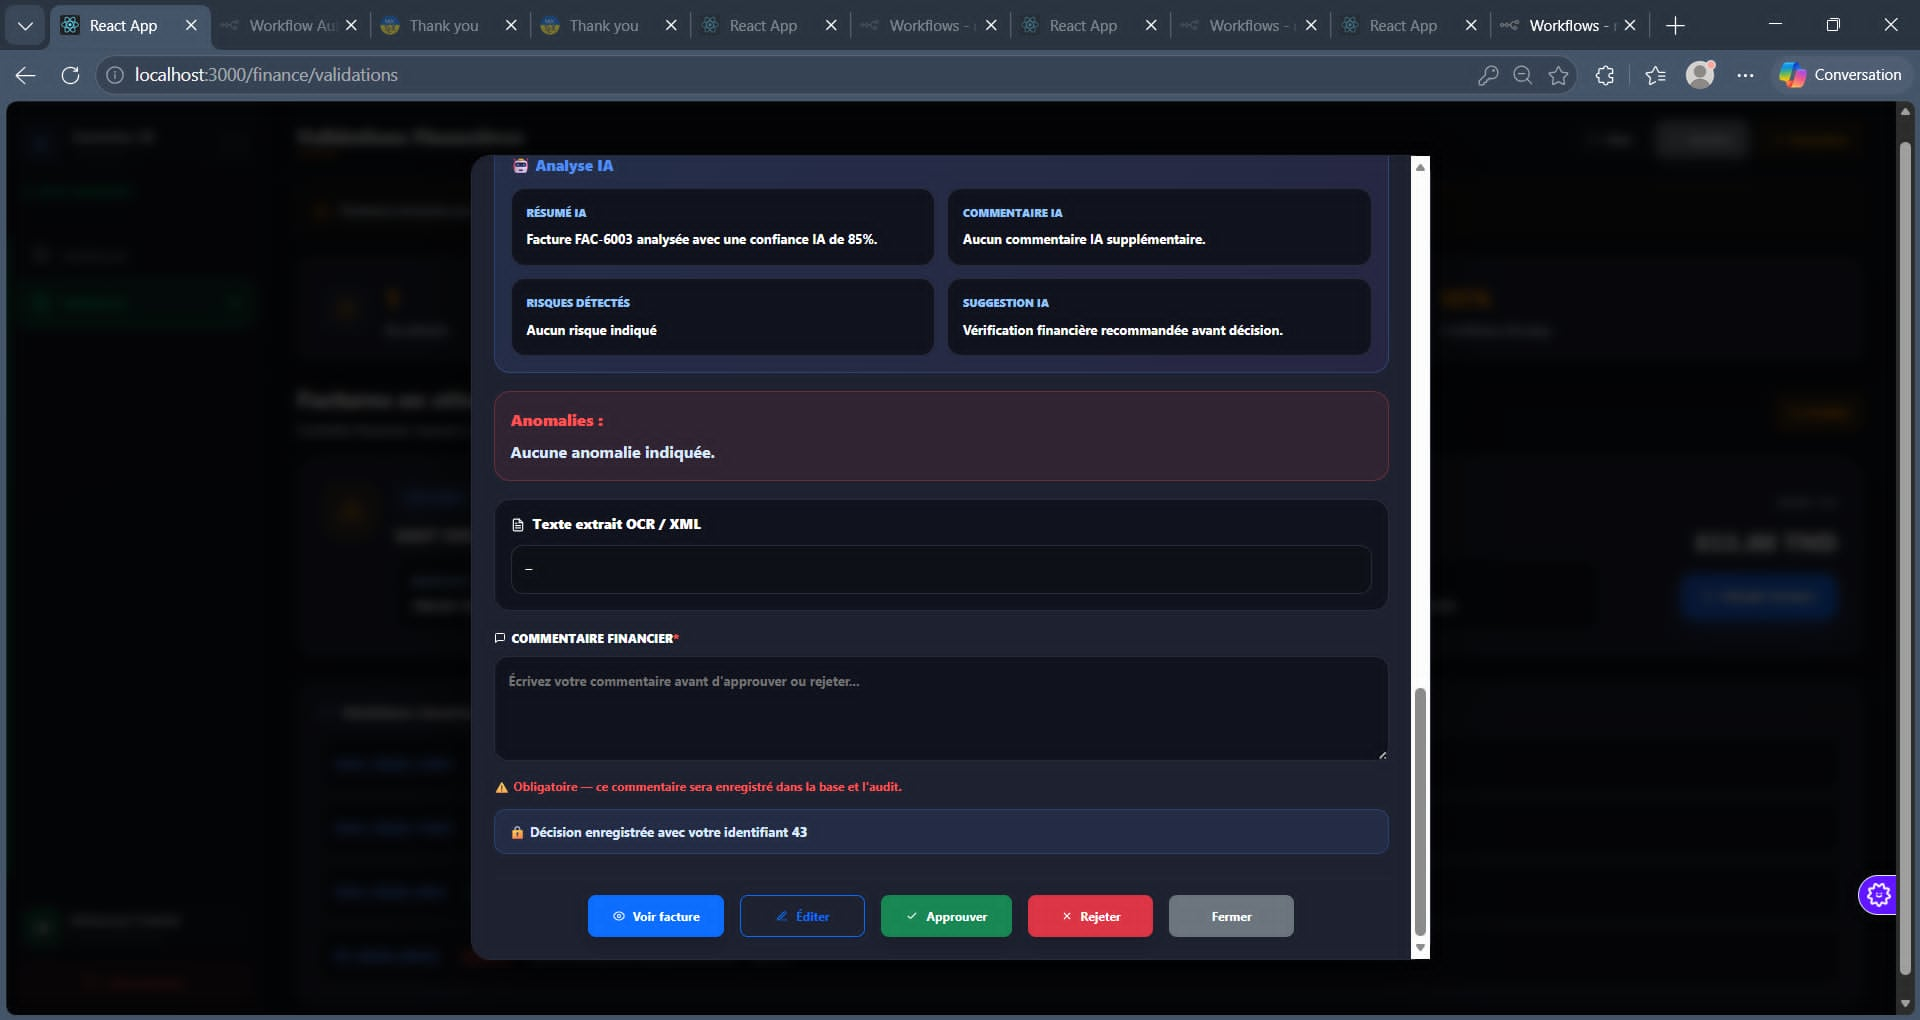
\includegraphics[width=0.85\textwidth]{ui_commentaire_obligatoire.jpg}
	\caption{Interface du commentaire obligatoire}
	\label{fig:ui_commentaire_obligatoire}
\end{figure}

\FloatBarrier

\subsubsection{Interface du tableau de bord financier}

Cette interface permet au responsable financier de visualiser les indicateurs financiers liés aux factures.

\begin{figure}[H]
	\centering
	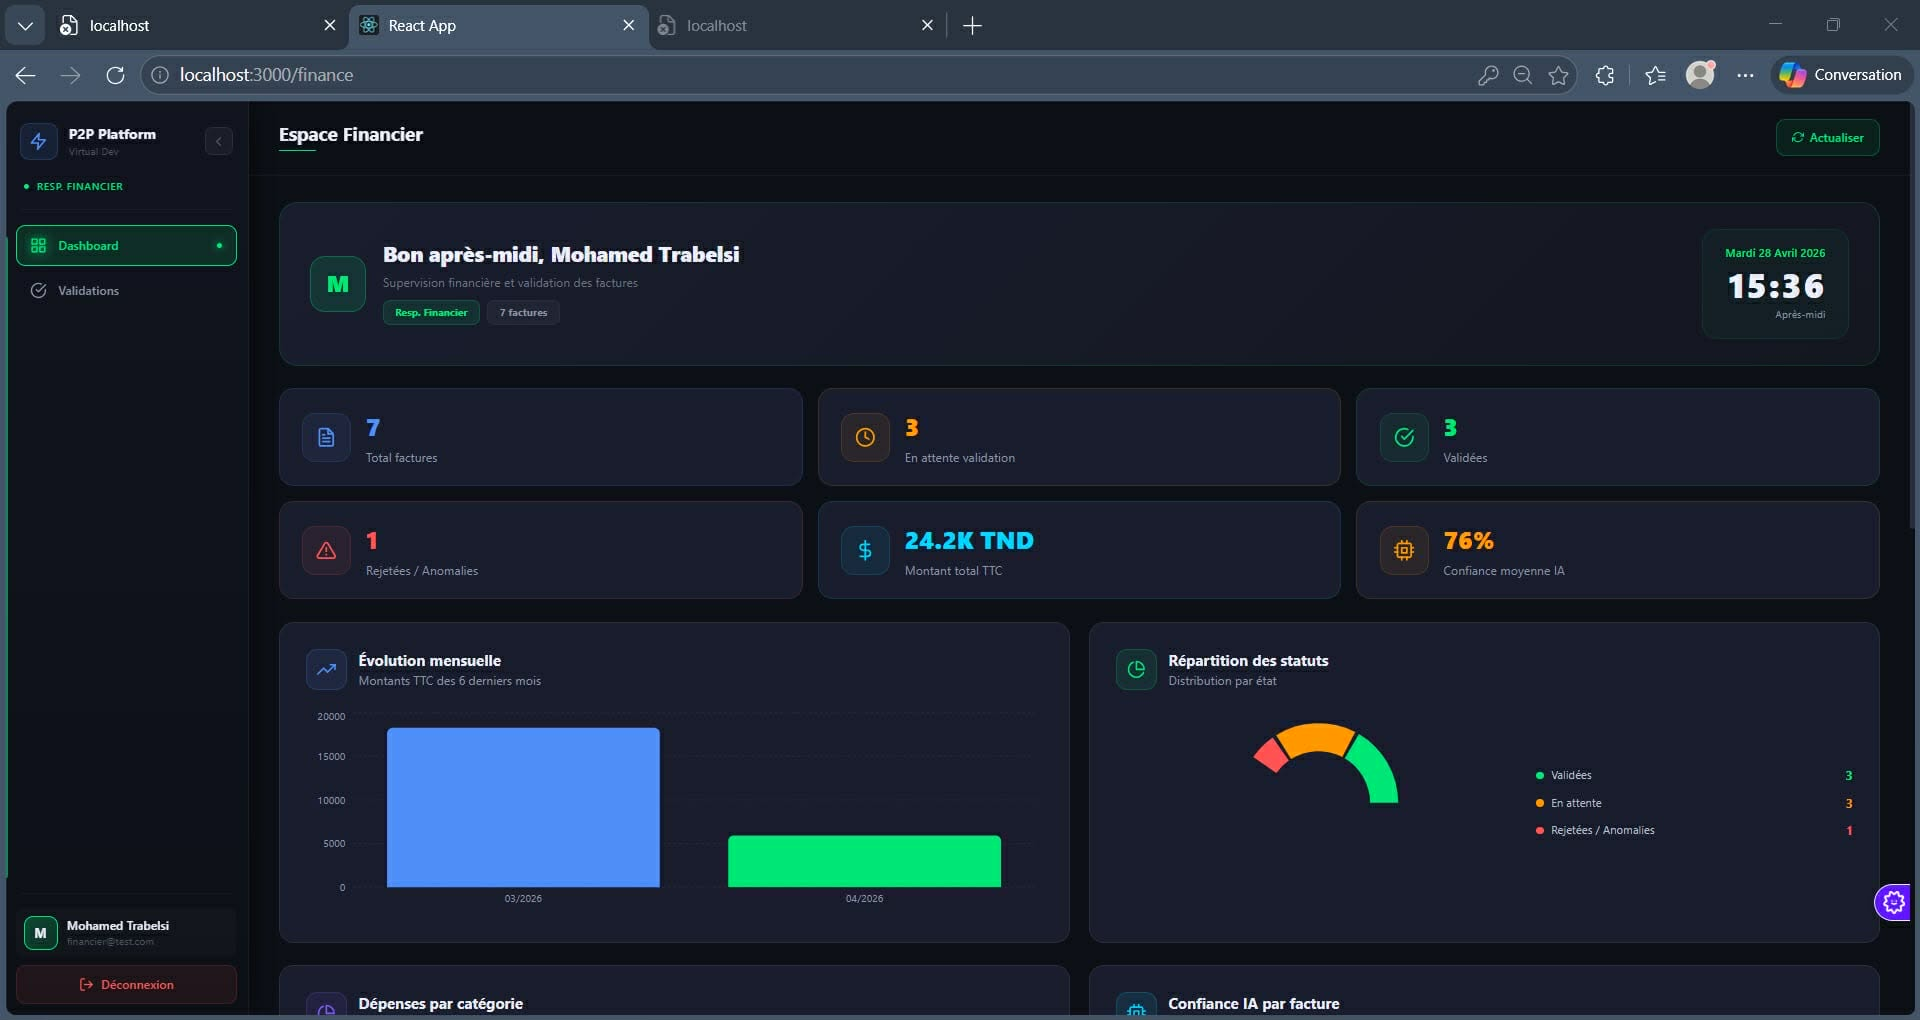
\includegraphics[width=0.65\textwidth]{ui_dashboard_financier.jpg}
	\caption{Interface du tableau de bord financier}
	\label{fig:ui_dashboard_financier}
\end{figure}

\FloatBarrier

\subsubsection{Interface du journal des actions}

Cette interface permet à l’administrateur de consulter l’historique des actions effectuées dans le système.

\begin{figure}[H]
	\centering
	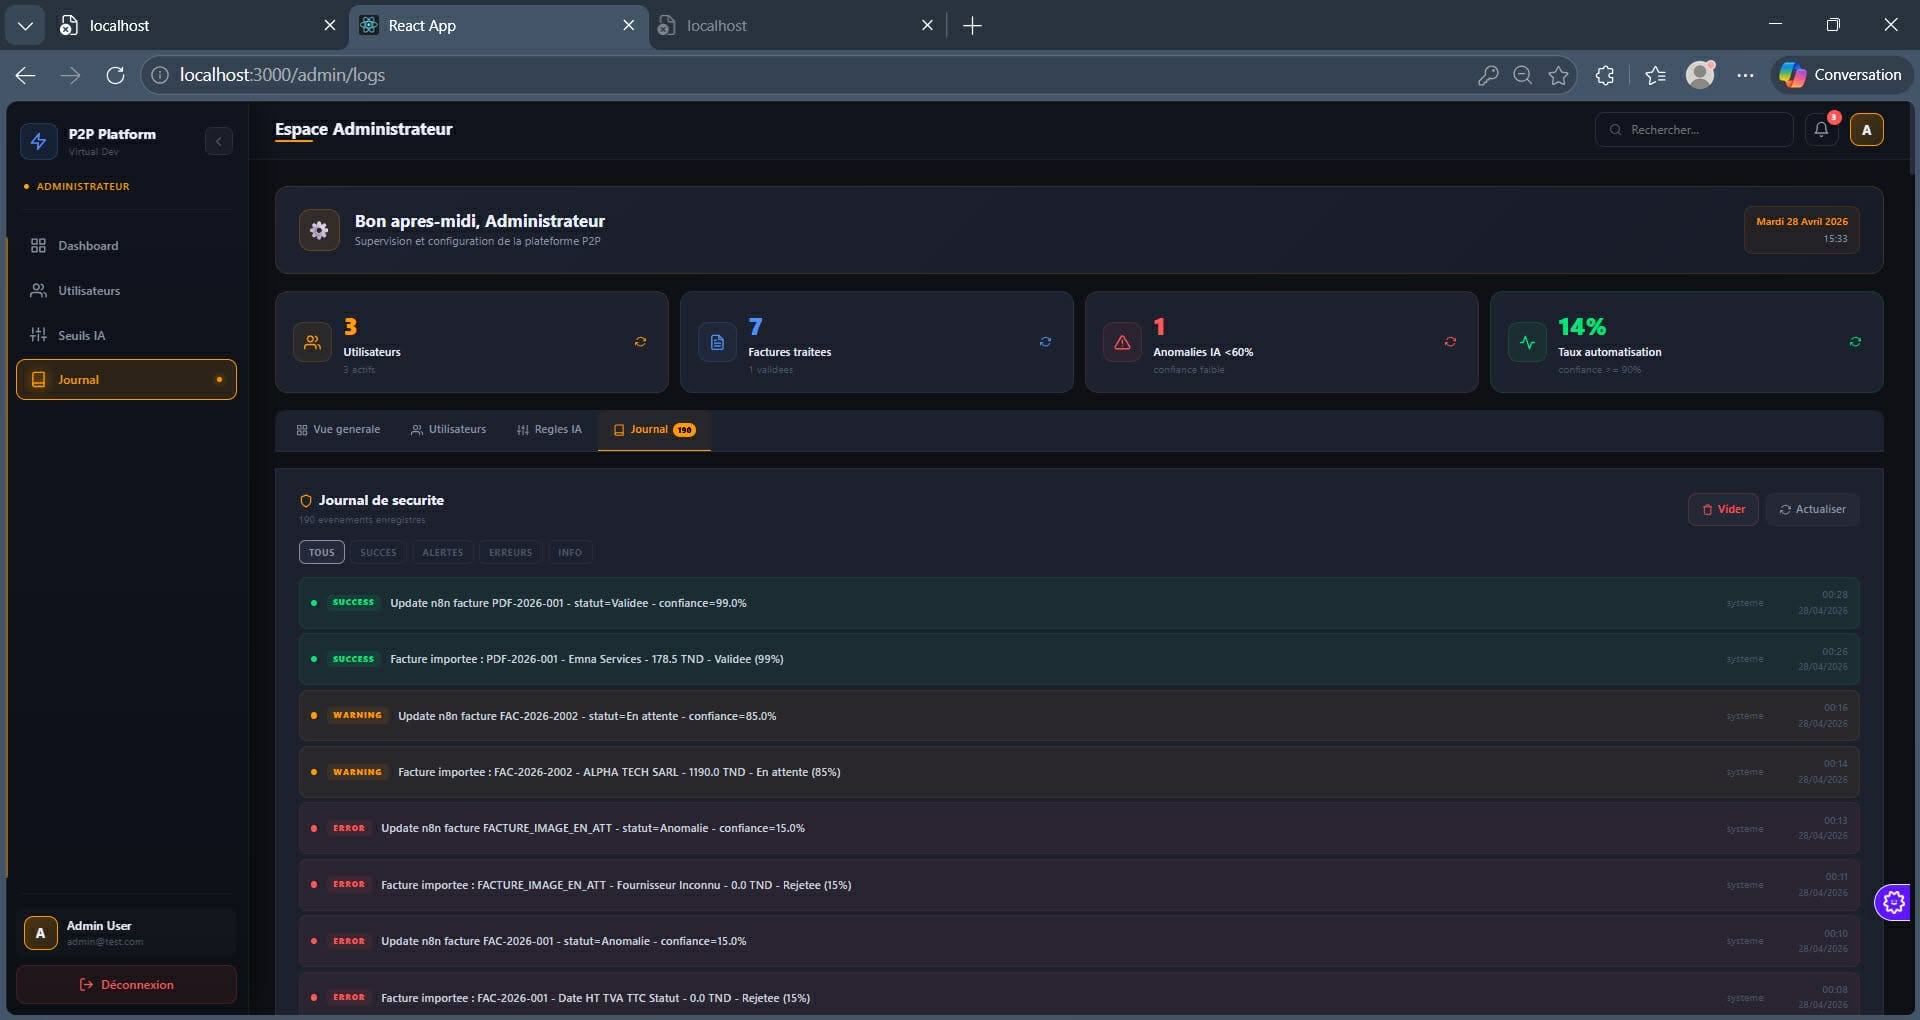
\includegraphics[width=0.85\textwidth]{ui_journal.jpg}
	\caption{Interface du journal des actions}
	\label{fig:ui_journal}
\end{figure}

\FloatBarrier

\section{Tests Postman}

Cette section présente les tests réalisés avec Postman afin de vérifier les fonctionnalités développées durant le Sprint 3.  
Ces tests concernent principalement la validation financière, le rejet des factures, l’affichage des statistiques et la configuration des seuils de confiance de l’intelligence artificielle.

L’objectif de ces tests est de confirmer que les décisions prises par le responsable financier sont correctement enregistrées et que les actions sont bien tracées dans le système.

\renewcommand{\arraystretch}{1.5}
\newpage
\begin{longtable}{|>{\centering\arraybackslash}m{5cm}|>{\centering\arraybackslash}m{9cm}|}
	\hline
	
	\rowcolor{blue!20}
	\textbf{Description} & \textbf{Capture}
	\\ \hline
	
	Cette requête permet au responsable financier de valider une facture. 
	Elle vérifie que le statut de la facture est mis à jour et que la décision est enregistrée avec un commentaire.
	&
	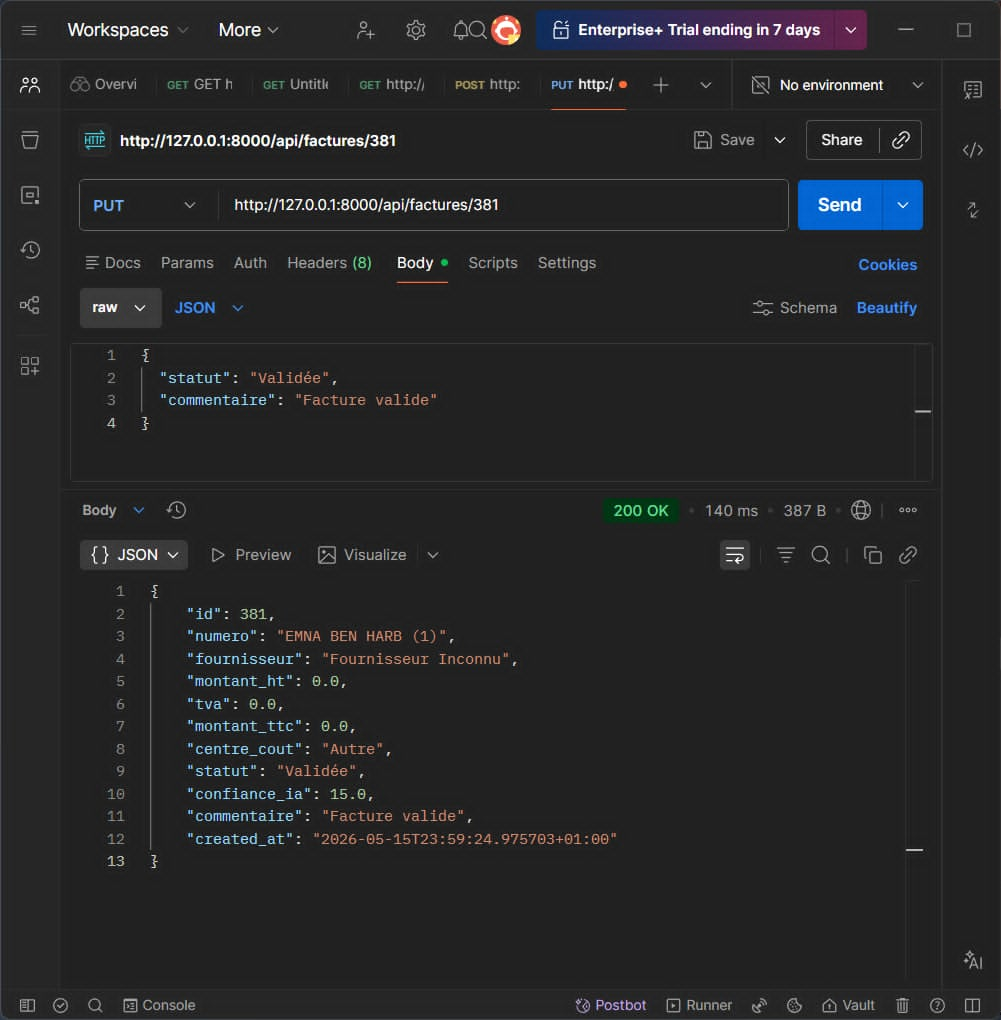
\includegraphics[width=8cm]{figures/postman_validation.jpg}
	\\ \hline
	
	Cette requête permet de rejeter une facture avec un commentaire obligatoire. 
	Elle permet de vérifier que le système refuse ou accepte la décision selon la présence du commentaire justificatif.
	&
	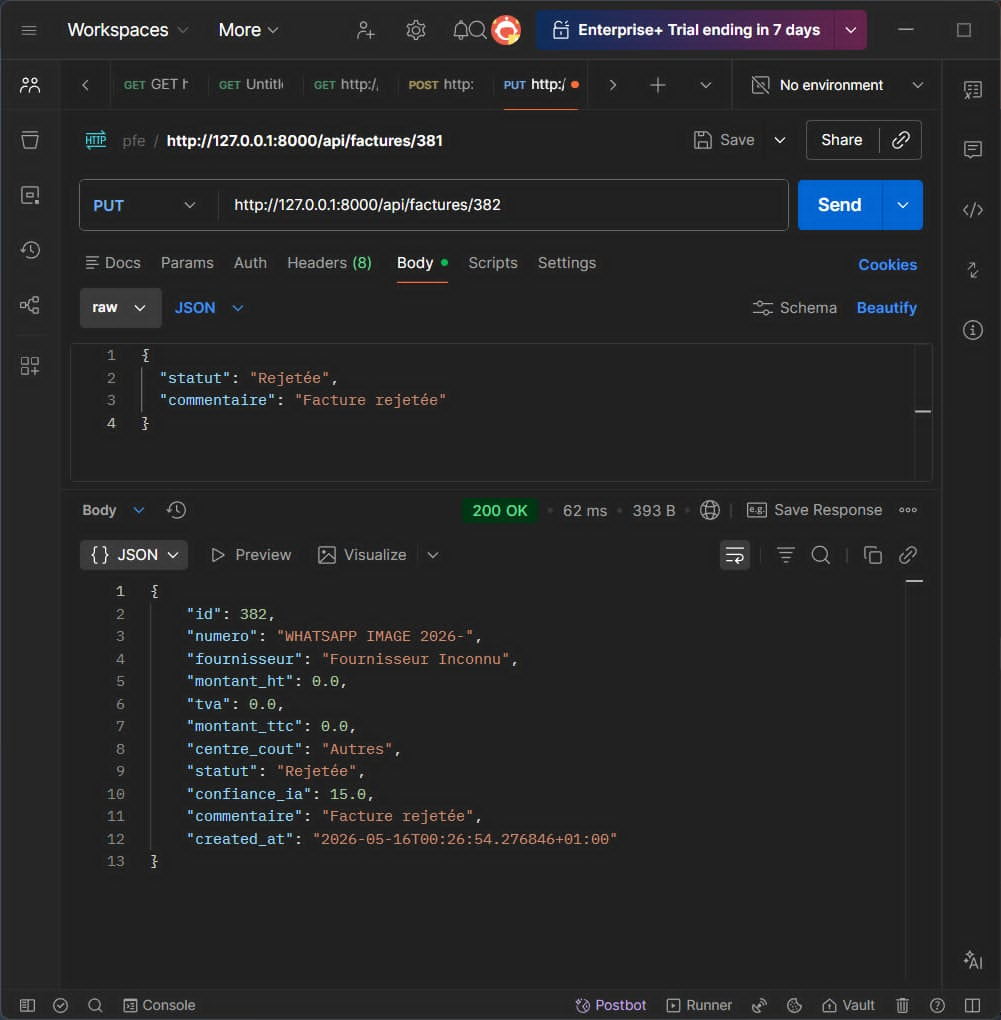
\includegraphics[width=8cm]{figures/postman_rejet.jpg}
	\\ \hline
	
	Cette requête permet d’afficher les statistiques et les indicateurs financiers. 
	Elle vérifie le bon fonctionnement du tableau de bord financier et la récupération des données nécessaires.
	&
	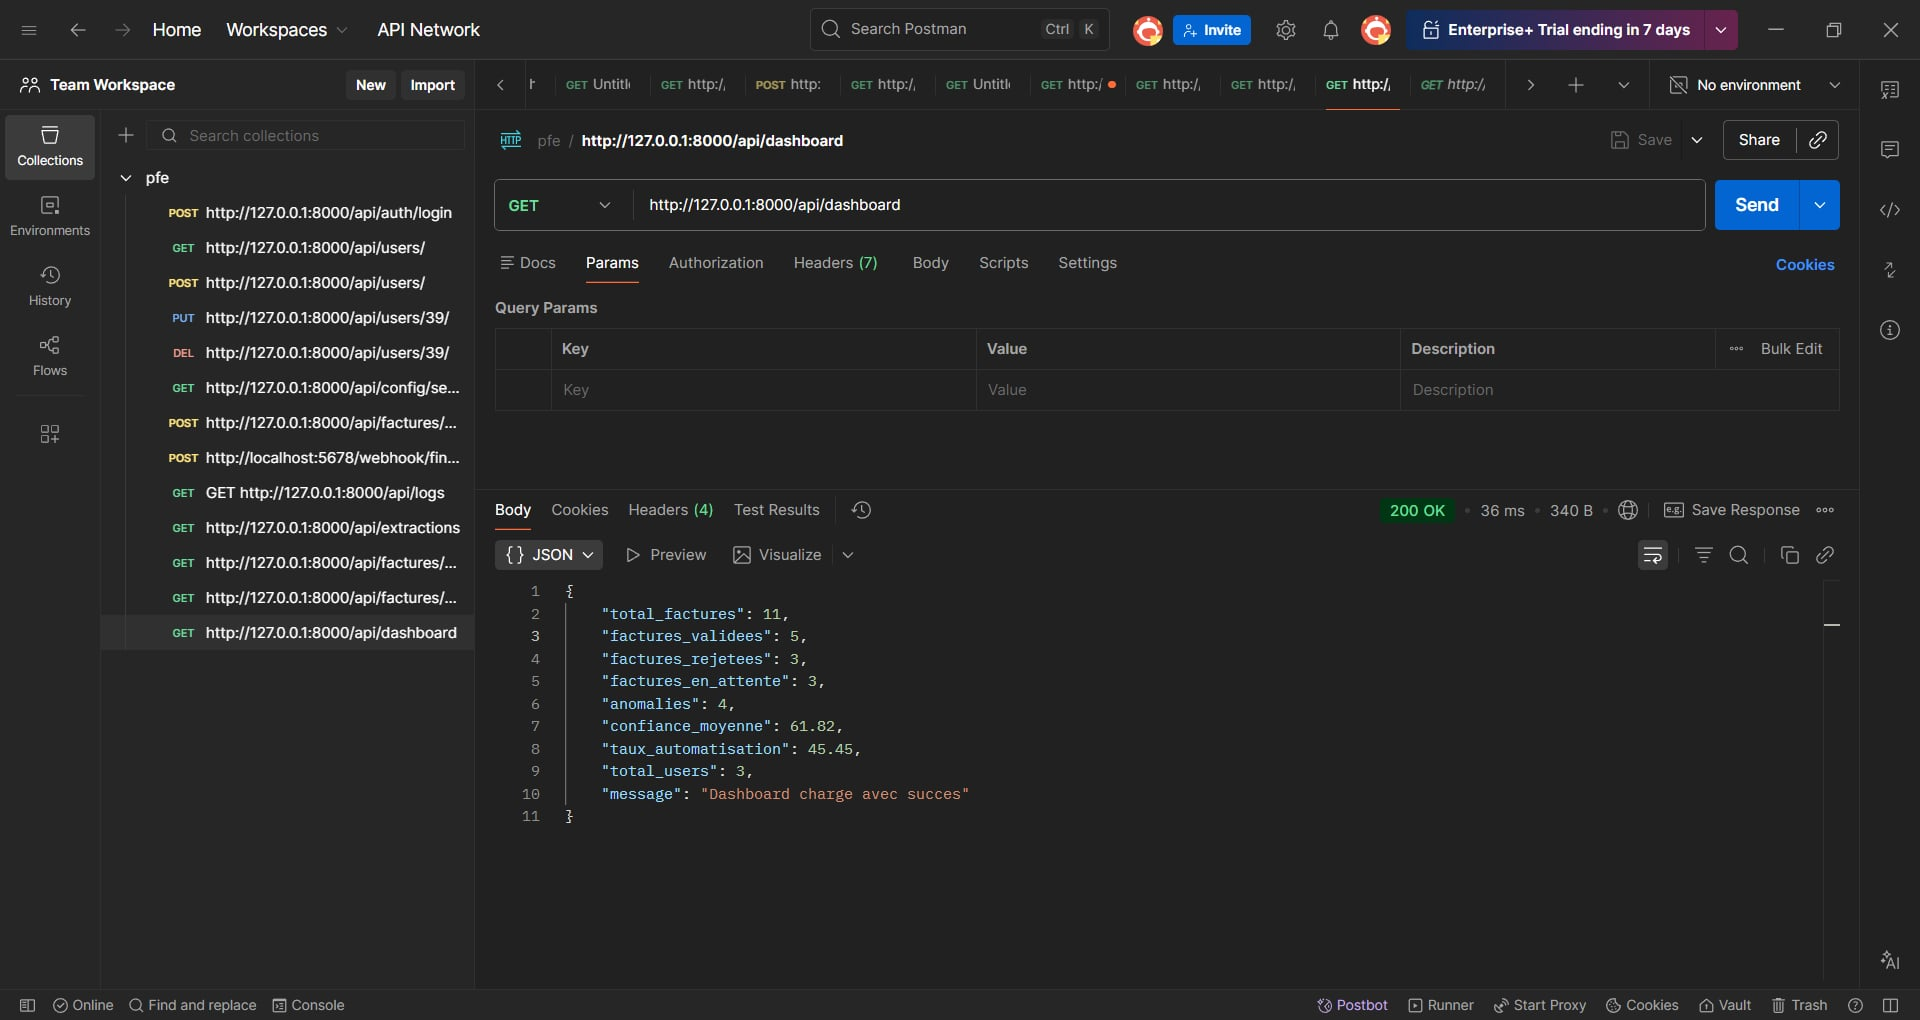
\includegraphics[width=8cm]{figures/postman_dashboard.jpg}
	\\ \hline
	
	Cette requête permet de modifier les seuils de confiance de l’intelligence artificielle. 
	Elle permet à l’administrateur d’ajuster les paramètres utilisés pour proposer automatiquement le statut d’une facture.
	&
	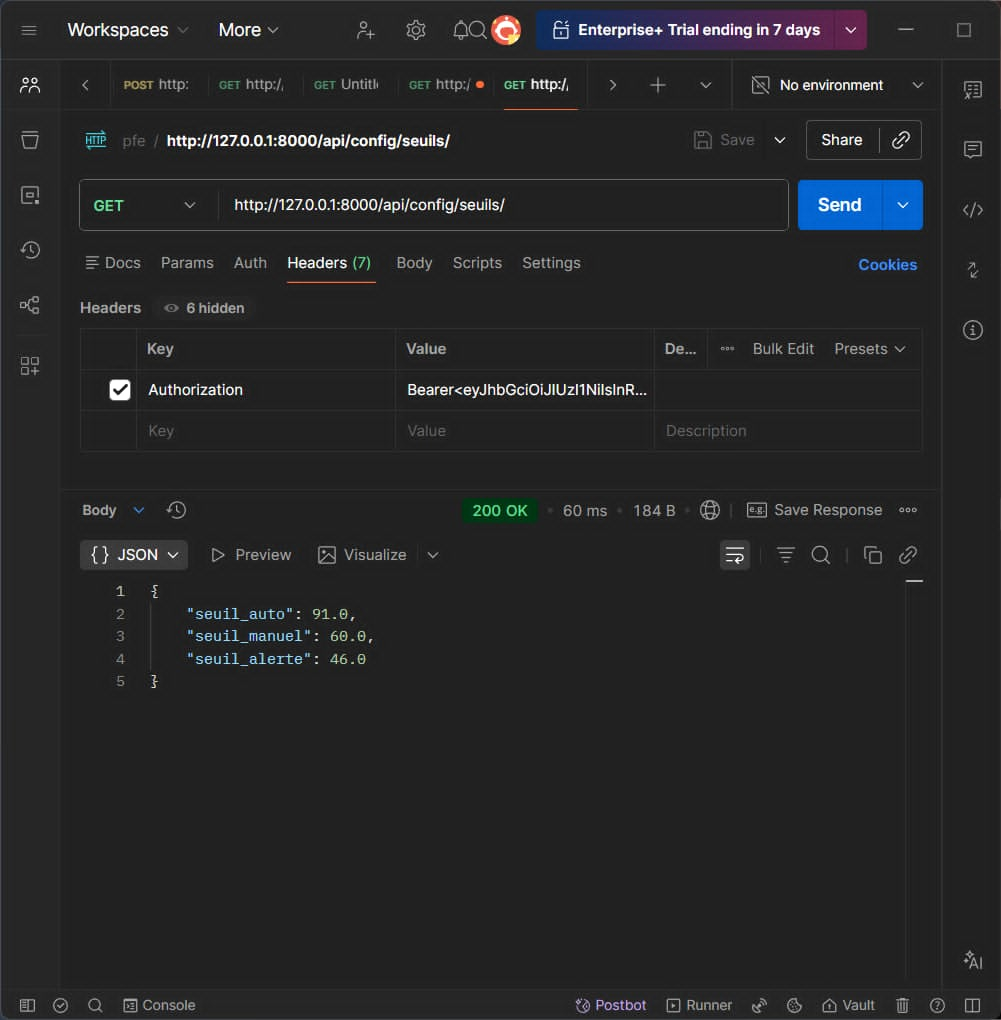
\includegraphics[width=8cm]{figures/postman_config_ia.jpg}
	\\ \hline
	
	\caption{Tests Postman du Sprint 3}
\end{longtable}
\vspace{0.3cm}
\subsection{Revue de Sprint}

La revue du Sprint 3 a permis de présenter les fonctionnalités réalisées concernant la validation financière des factures, la gestion des commentaires obligatoires ainsi que la traçabilité des actions à travers le journal des opérations. Cette étape a permis de vérifier le bon fonctionnement des processus de validation, de rejet et d’enregistrement des actions dans le système.
\vspace{0.1cm}
\paragraph{Burndown Chart :}

Le Burndown Chart du Sprint 3 illustre l’évolution du travail restant durant les fonctionnalités de validation financière et de traçabilité. Le graphique montre la progression des tâches réalisées et le respect du planning
prévu pour ce sprint. Comme présenté dans la figure \ref{fig:brun2}.
\begin{figure}[H]
	\centering
	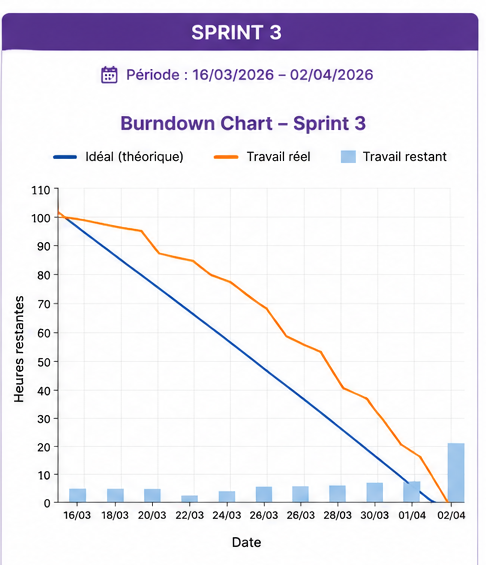
\includegraphics[width=0.5\textwidth]{burndown_sprint3.jpg}
	\caption{Diagramme de Burndown Chart du Sprint 3}
	\label{fig:brun3}
\end{figure}
\begin{table}[H]
	\centering
	\renewcommand{\arraystretch}{1.3}
	
	\begin{tabular}{|c|p{5cm}|c|}
		\hline
		\rowcolor{blue!20}
		\textbf{ID User Story} & \textbf{Fonctionnalité} & \textbf{Estimation} \\
		\hline
		
		3.1 & Validation financière des factures & 5 \\
		\hline
		
		3.2 & Rejet avec commentaire obligatoire & 3 \\
		\hline
		
		3.3 & Journal des actions & 4 \\
		\hline
		
		3.4 & Tableau de bord financier & 4 \\
		\hline
		
		3.5 & Gestion des statistiques & 3 \\
		\hline
		
		3.6 & Finalisation et tests globaux & 3 \\
		\hline
		
		\multicolumn{2}{|c|}{\textbf{Vélocité totale estimée}} & \textbf{22} \\
		\hline
		
	\end{tabular}
	
	\caption{Calcul de vélocité estimée du Sprint 3}
\end{table}
\section{Conclusion}

Dans ce chapitre, nous avons présenté les fonctionnalités réalisées durant le Sprint 3. Nous avons développé les mécanismes de validation financière, la gestion des anomalies ainsi que la traçabilité des actions afin d’assurer un meilleur suivi des opérations du système.
\chapter*{Conclusion générale}
\addcontentsline{toc}{chapter}{Conclusion générale}

Ce projet de fin d’études réalisé dans le cadre de notre stage au sein de l’entreprise Virtual Dev nous a permis de mettre en pratique les connaissances acquises durant notre parcours universitaire et de développer davantage nos compétences techniques et professionnelles dans le domaine du développement logiciel.

L’objectif principal de ce projet était la conception et le développement d’une plateforme intelligente de gestion et de validation des factures fournisseurs basée sur les technologies web, l’OCR et l’intelligence artificielle. Cette solution a été proposée afin d’automatiser le traitement des factures, réduire les tâches manuelles et améliorer l’efficacité du processus de validation financière.

Tout au long de ce travail, nous avons commencé par étudier l’existant et identifier les différentes limites du traitement manuel des factures, notamment la perte de temps, les erreurs humaines et le manque de traçabilité. Ensuite, nous avons analysé les besoins fonctionnels et non fonctionnels du système afin de proposer une architecture adaptée et performante.

La réalisation de ce projet nous a également permis d’utiliser plusieurs technologies modernes telles que React pour le frontend, FastAPI pour le backend, PostgreSQL pour la gestion de la base de données ainsi que les outils OCR et IA pour l’extraction et l’analyse automatique des données. Nous avons aussi adopté la méthodologie agile SCRUM afin d’assurer une meilleure organisation du travail et un suivi efficace de l’avancement du projet.

La plateforme développée offre plusieurs fonctionnalités importantes, notamment l’importation des factures, l’extraction automatique des données, la validation financière, la gestion des utilisateurs, le suivi des actions et la visualisation des statistiques via des tableaux de bord interactifs. Cette solution permet ainsi d’améliorer la rapidité, la fiabilité et la sécurité du traitement des factures au sein de l’entreprise.

Ce projet représente une expérience très enrichissante aussi bien sur le plan technique que professionnel. Il nous a permis de travailler sur un projet concret, de résoudre plusieurs problèmes techniques et de découvrir de nouvelles technologies utilisées dans le domaine des systèmes intelligents.

Comme perspectives d’amélioration, il serait intéressant d’ajouter de nouvelles fonctionnalités telles qu’un système avancé de notification, une analyse intelligente plus poussée des anomalies, ainsi qu’une intégration avec d’autres systèmes de gestion d’entreprise afin d’améliorer davantage les performances et les capacités de la plateforme.

En conclusion, ce projet constitue une étape importante dans notre parcours académique et professionnel. Les résultats obtenus répondent aux objectifs fixés et représentent une base solide pour de futures améliorations et évolutions du système.

%\printbibliography[nottype=online, title=Bibliographie]
%\printbibliography[type=online, title=Webographie]

\end{document}